In the following sections we present the preliminary analysis and the machine and deep learning study applied to the predictions of the Hodge numbers of \cicy $3$-folds.
We use both a ``classical'' approach to \ml using \emph{shallow learning} algorithm using geometrical methods to find new representations of the data and more moder approaches based on \emph{computer vision} and recent developments in computer science techniques.
We show how \emph{deep learning} the geometry of string theory can help in providing good computational tools for phenomenology and algebraic geometry.
We also stress future investigations which can be performed based on these results.


\subsection{Exploratory Data Analysis}
\label{sec:data:eda}

A typical \ml project does not consist of feeding the raw data to the algorithm.
It is instead preceded by a phase of exploration in order to better understand the data, which in turn can help to design the learning algorithms.
We call \emph{features} properties given as inputs, and \emph{labels} the targets of the predictions.
There are several phases in the exploratory data analysis (\eda)~\cite{Skiena:2017:DataScienceDesign}:
\begin{enumerate}
  \item \emph{feature engineering}: new features are derived from the inputs;

  \item \emph{feature selection}: the most relevant features are chosen to explain the targets;

  \item \emph{data augmentation}: new training data is generated from the existing ones;

  \item \emph{data diminution}: part of the training data is not used.
\end{enumerate}

Engineered features are redundant by definition but they can help the algorithm learn more efficiently by providing an alternative formulation and by drawing attention on salient characteristics.
A simple example is the following: given a series of numbers, one can compute different statistics, such as median, mean and variance, and add them to the inputs.
It may happen that the initial series becomes then irrelevant once this new information is introduced.
Another approach to improve the learning process is to augment or decrease the number of training samples artificially.\footnotemark{}
\footnotetext{%
  This is in general used in computer vision and object detection tasks where providing rotated, scaled and cropped versions of the input images can help the algorithms in learning more representations of the same object, thus creating more accurate predictions.
}
For example we could use invariances of the inputs to generate more training data.
This however does not help in our case because the entries of the configuration matrices are partially ordered.
Another possibility is to remove outliers which can damage the learning process by driving the algorithm far from the best solution.
If there are few of them it is better to ignore them altogether during training since an algorithm which is not robust to outliers will in any case make bad predictions (a standard illustration is given by the Pearson and Spearman correlation coefficients, with the first not being robust to outliers~\cite{Skiena:2017:DataScienceDesign}).

Before starting the \eda, the first step should be to split the data into training and validation sets to avoid biasing the choices of the algorithm and the strategy: the \eda should be performed only on the training set.
However the dataset we consider is complete and quite uniform: a subset of it would display the same characteristics as the entire set.\footnotemark{}
\footnotetext{%
  A dataset is \emph{tidy} if every column represents a separate variable and every row is a different observation.
  For instance every row could represent a date expressed in seconds from a reference instant and every column could be a separate sensor reading.
  However the ``transposed'' version of the dataset is not a tidy dataset because the observations are in the columns, thus representing a non standard form of the data.
  A tidy dataset is \emph{complete} if there are no empty cells, that is there is no lack of data or information in the entire set.
  A \emph{uniform} dataset can be understood as a complete dataset in which every variable is well distributed and does not present a lot of outliers or anomalies.
}
To give a general overview of the properties we work with the full dataset.


\subsubsection{Engineering}

\begin{figure}[tbp]
  \centering
  \begin{subfigure}[c]{.45\linewidth}
    \centering
    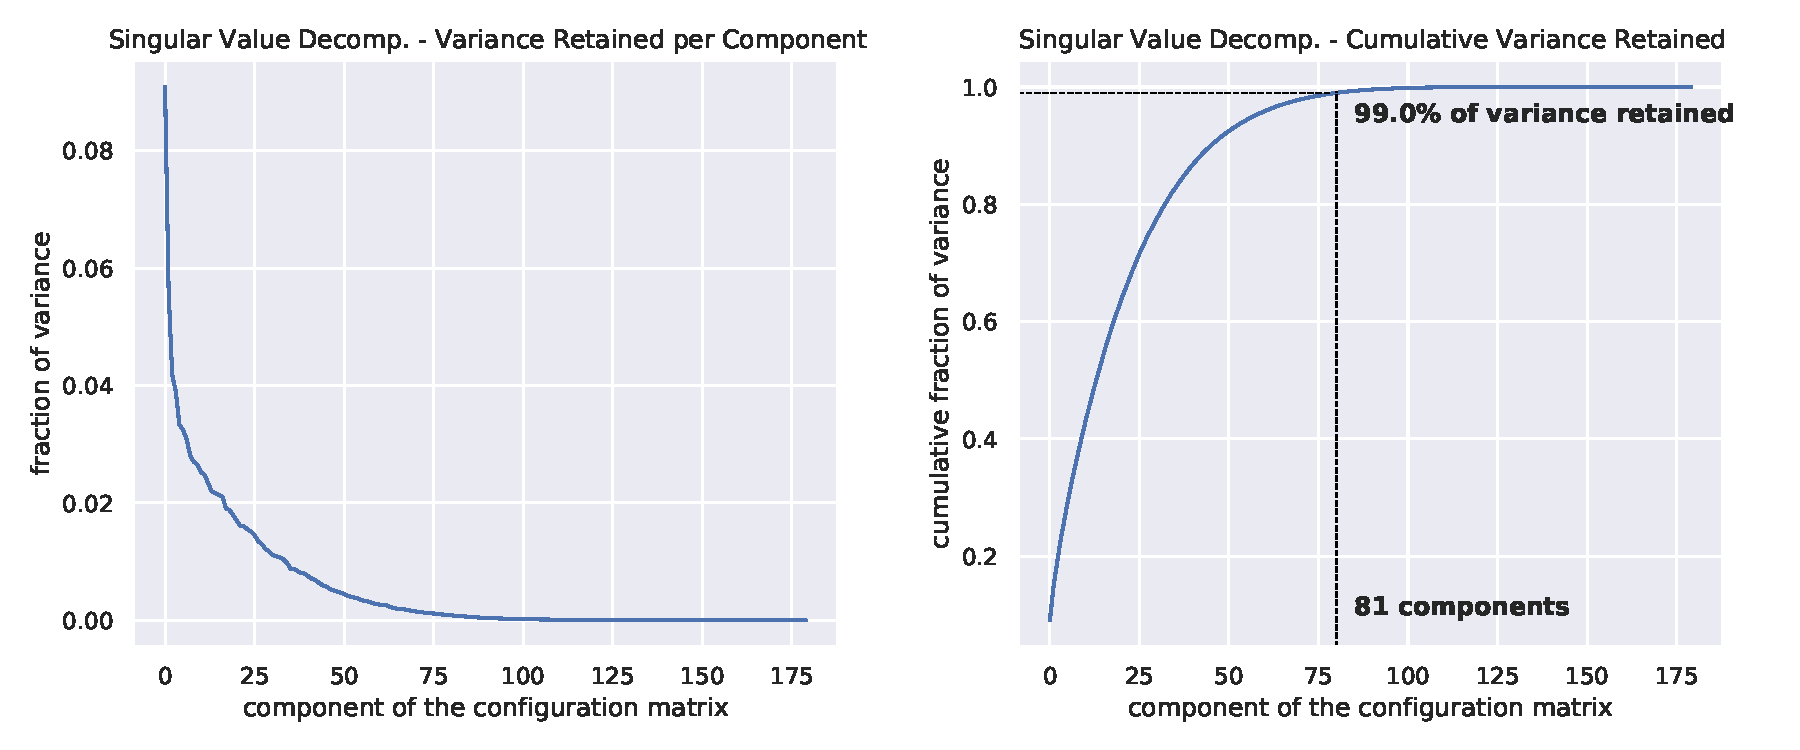
\includegraphics[width=\linewidth, trim={6in 0 0 0}, clip]{img/svd_orig}
    \caption{original dataset}
  \end{subfigure}
  \hfill
  \begin{subfigure}[c]{.45\linewidth}
    \centering
    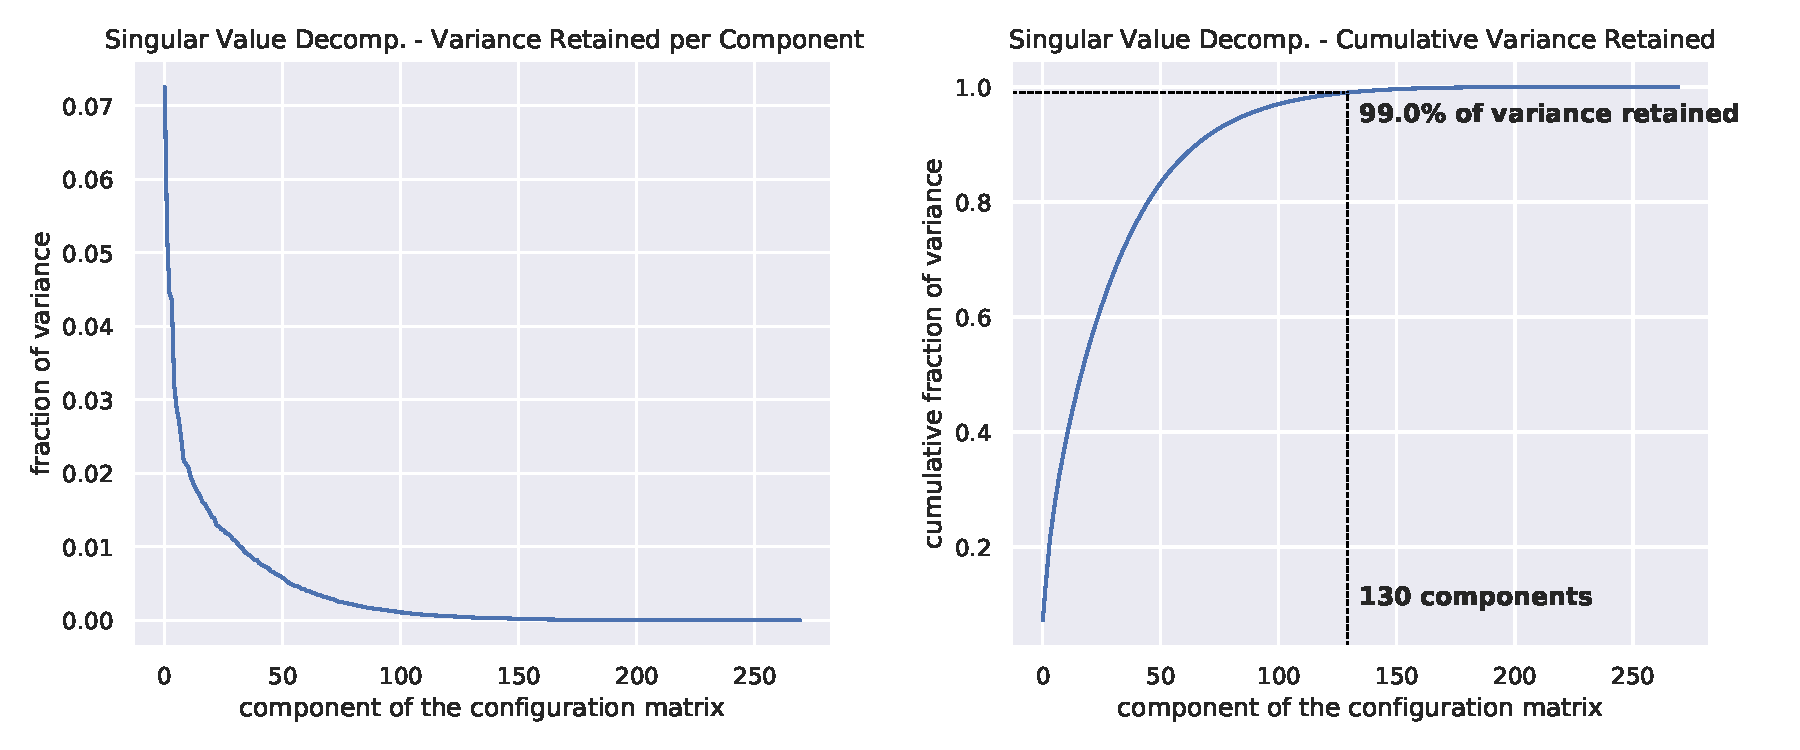
\includegraphics[width=\linewidth, trim={6in 0 0 0}, clip]{img/svd_fav}
    \caption{favourable dataset}
  \end{subfigure}
  \caption{%
    Cumulative retained variance of the principal components of the configuration matrix.
  }
  \label{fig:eda:svd}
\end{figure}

Any transformation of the input data which has some mathematical meaning can be a useful feature.
We establish the following list of useful quantities (most of them are already used to characterise \cicy manifolds in the literature~\cite{Hubsch:1992:CalabiyauManifoldsBestiary}):
\begin{itemize}
  \item the number of projective spaces (rows), $m = $ \texttt{num\_cp};

  \item the number of equations (columns), $k = $ \texttt{num\_eqs};

  \item the number of $\mathds{P}^1$, $f = $ \texttt{num\_cp\_1};

  \item the number of $\mathds{P}^2$, \texttt{num\_cp\_2};

  \item the number of $\mathds{P}^n$ with $n \neq 1$, $F = $ \texttt{num\_cp\_neq1};

  \item the excess number $N_{ex} = \finitesum{r}{1}{F} \qty(n_r + f + m - 2k) =$ \texttt{num\_ex};

  \item the dimension of the cohomology group $H^0$ of the ambient space, \texttt{dim\_h0\_amb};

  \item the Frobenius norm of the matrix, \texttt{norm\_matrix};

  \item the list of the projective space dimensions \texttt{dim\_cp} and statistics thereof (min, max, median, mean);

  \item the list of the equation degrees \texttt{deg\_eqs} and statistics thereof (min, max, median, mean);

  \item $k$-means clustering on the components of the configuration matrix (with a number of clusters going from 2 to 15);\footnotemark{}
  \footnotetext{%
    The algorithm determines the centroids of conglomerates of data called \textit{clusters} using an iterative process which computes the distance of each sample from the center of the cluster.
    It then assigns the label of the cluster to the nearest samples.
    We use the class \texttt{cluster.KMeans} in \texttt{scikit-learn}.
  }%

  \item principal components of the configuration matrix derived using a principal components analysis (\pca) with \SI{99}{\percent} of the variance retained (see~\Cref{fig:eda:svd}).
\end{itemize}


\subsubsection{Selection}


\paragraph{Correlations}

To get a first general idea it is useful to take a look at the correlation matrix of the features and the labels.\footnotemark{}
\footnotetext{%
  The correlation is defined as the ratio between the covariance of two variables $\sigma(x, y) = \sum_{i} (x_i - \bar{x})(y_i - \bar{y})$ and the product of the standard deviations $\sigma(x)\sigma(y)$ (in this case $\bar{x}$ and $\bar{y}$ are the sample means).
}
The correlation matrices for the scalar variables are displayed in~\Cref{fig:eda:corr} for the original and favourable datasets (this excludes the configuration matrix).
As we can see some engineered features are strongly correlated, especially in the favourable dataset.
In particular \hodge{1}{1} (respectively \hodge{2}{1}) is strongly correlated (respectively anti-correlated) with the number of projective spaces $m$ and with the norm and rank of the matrix.
This gives a first hint that these variables could help improve predictions by feeding them to the algorithm along with the matrix.
On the other hand finer information on the number of projective spaces and equations do not correlate with the Hodge numbers.

From this analysis, and in particular from~\Cref{fig:eda:corr}, we find that the values of \hodge{1}{1} and \hodge{2}{1} are also correlated.
This motivates the simultaneous learning of both Hodge numbers since it can increase chances for the neural network to learn more universal features.
In fact this is something that often happens in practice: it has been found that multi-tasking enhances the ability to generalise~\cite{Thrun:1996:LearningNthThing, Caruana:1997:MultitaskLearning, Baxter:2000:ModelInductiveBias, Maurer:2016:BenefitMultitaskRepresentation, Ndirango:2019:GeneralizationMultitaskDeep}.

\begin{figure}[tbp]
  \centering
  \begin{subfigure}[c]{.45\linewidth}
    \centering
    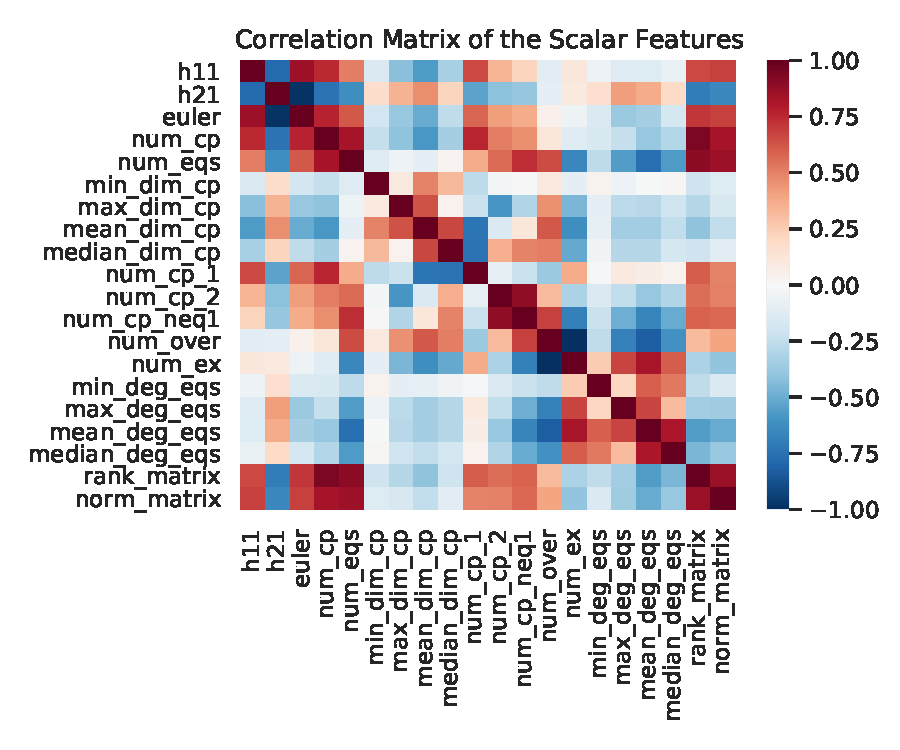
\includegraphics[width=\linewidth]{img/corr-matrix_orig}
    \caption{original dataset}
  \end{subfigure}
  \hfill
  \begin{subfigure}[c]{.45\linewidth}
    \centering
    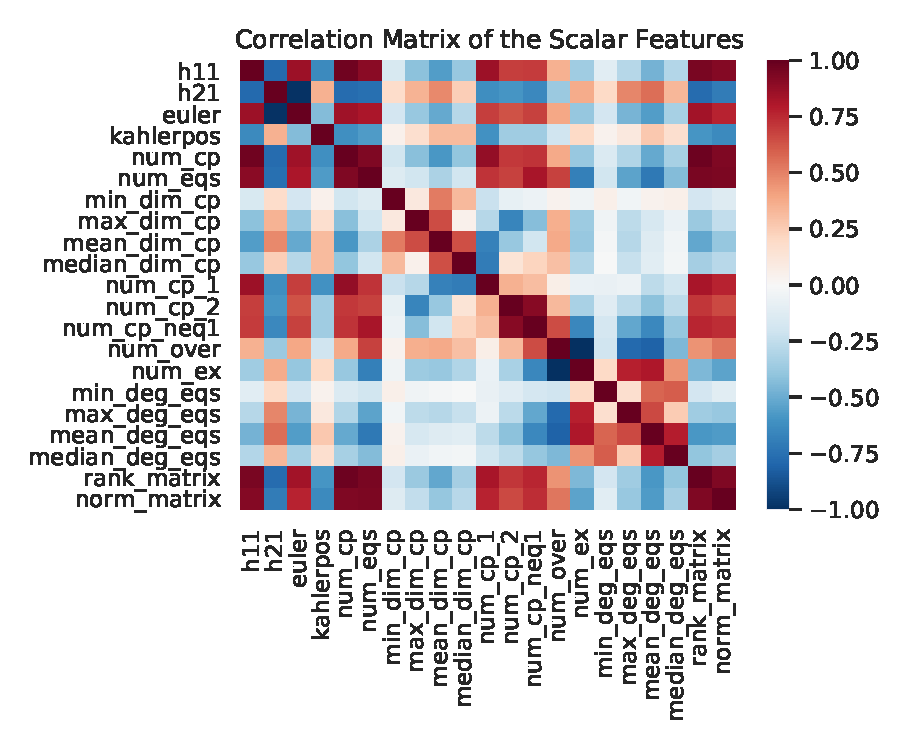
\includegraphics[width=\linewidth]{img/corr-matrix_fav}
    \caption{favourable dataset}
  \end{subfigure}
  \caption{Correlations between the engineered scalar features and the labels.}
  \label{fig:eda:corr}
\end{figure}


\paragraph{Feature importance}

A second non-exclusive option is to sort the features by order of importance.
This can be done using a decision tree which is capable to determine the weight of each variable towards making a prediction.
One advantage over correlations is that the algorithm is non-linear and can thus determine subtler relations between the features and labels.
To avoid biasing the results using only one decision tree, we trained a random forest of trees (using \texttt{ensemble.RandomForestRegressor} in \texttt{scikit-learn}).
It consists in a large number of decision trees which are trained on different random subsets of the training dataset and averaged over the outputs (see~\Cref{sec:app:trees} for details on the implementation).
The algorithm determines the importance of the different features to make predictions as a by-product of the learning process: the most relevant features tend to be found at the first branches (or to be used the most) since they are the most important to make the prediction.
The importance of a variable is a number between $0$ and $1$, and the sum over all of them must be $1$.
Since a random forest contains many trees the robustness of the variable ranking usually improves with respect to a single tree (\Cref{sec:app:trees}).
Moreover, as the main objective is to obtain a qualitative preliminary understanding of the features, there is no need for fine tuning at this stage and we use the default parameters (specifically \num{100} decision trees).
We computed feature importance for both datasets and for two different set of variables: one containing the engineered features and the configuration matrix, and one with the engineered features and the \pca components.
In the following figures, we show several comparisons of the importance of the features, dividing the figures into scalars, vectors and configuration matrix (or its \pca), and clusters.
The sum of importance of all features equals $1$.

In~\Cref{fig:eda:scalars}, we show the ranking of the scalar features in the two datasets (differences between the set using the configuration matrix and the other using the \pca are marginal and are not shown to avoid redundant plots).
As already mentioned we find that the number of projective spaces is the most important feature by far.
It is followed by the matrix norm in the original dataset, and by the matrix rank for \hodge{2}{1} in the favourable dataset.
Finally the variable ranking points out that the other features have a negligible impact on the determination of the labels and may as well be ignored during training.

\begin{figure}[tbp]
  \centering
  \begin{subfigure}[c]{0.45\linewidth}
    \centering
    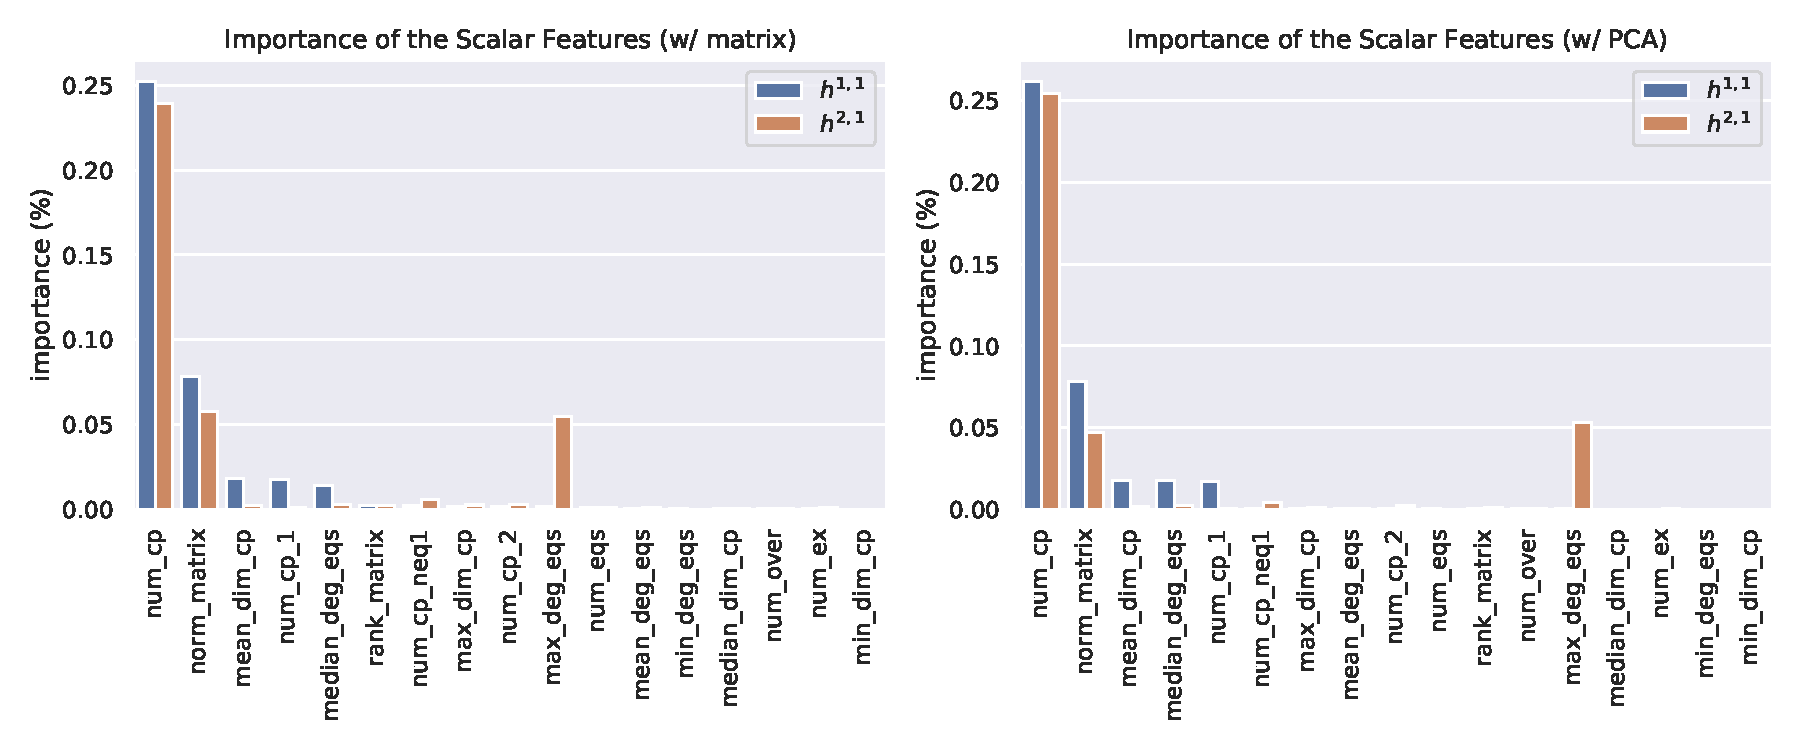
\includegraphics[width=\linewidth, trim={0 0 6in 0}, clip]{img/scalar-features_orig}
    \caption{original dataset}
  \end{subfigure}
  \hfill
  \begin{subfigure}[c]{0.45\linewidth}
    \centering
    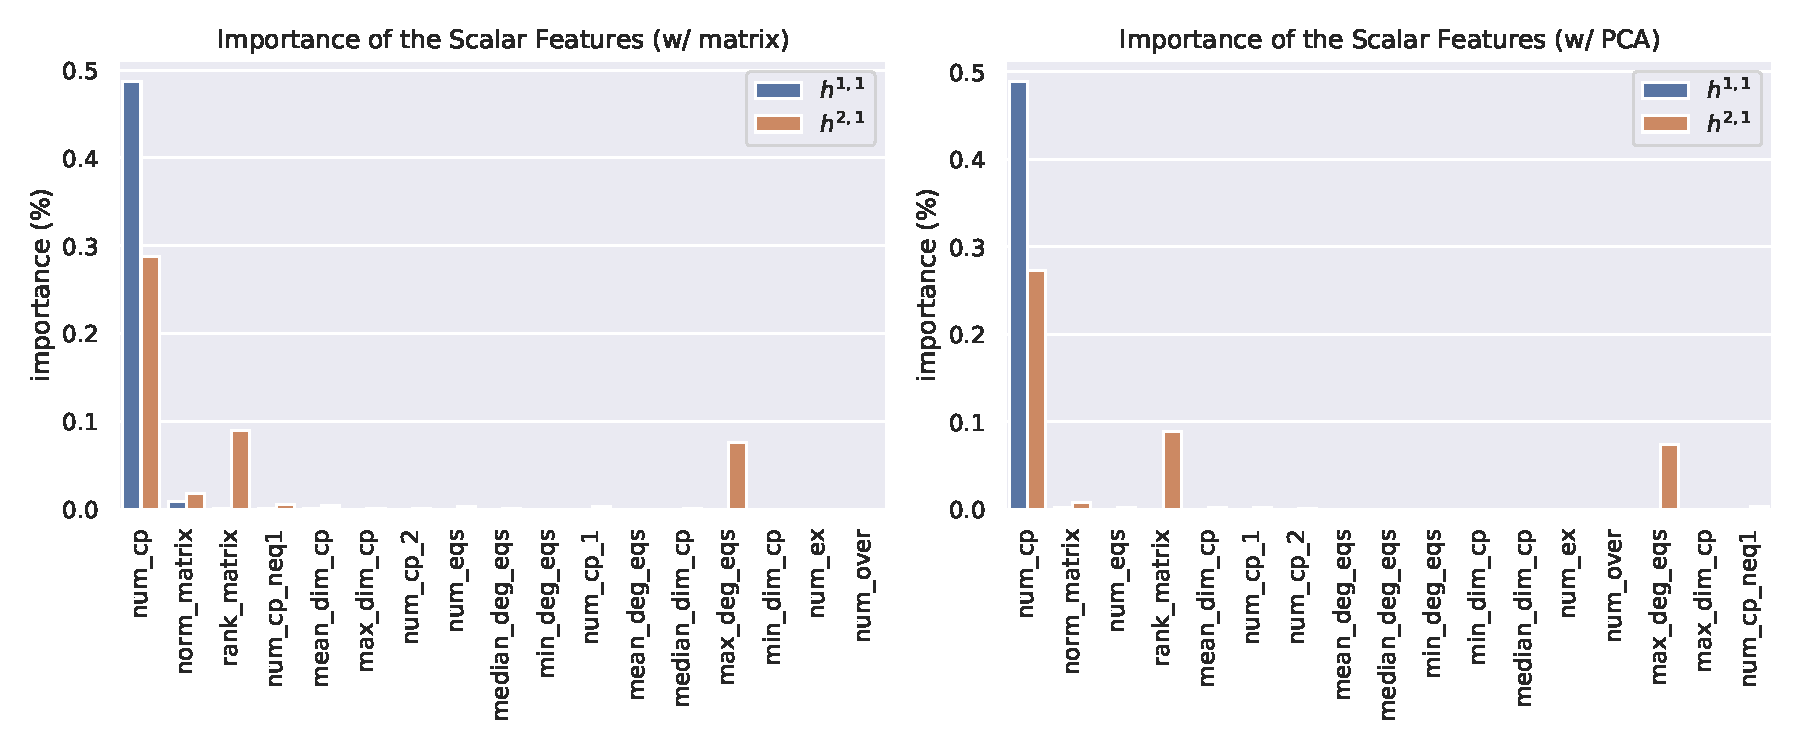
\includegraphics[width=\linewidth, trim={0 0 6in 0}, clip]{img/scalar-features_fav}
    \caption{favourable dataset}
  \end{subfigure}
  \caption{%
    Importance of the scalar features in the datasets.
  }
  \label{fig:eda:scalars}
\end{figure}

The same analysis can be repeated for the vector features and the configuration matrix component by component.
In~\Cref{fig:eda:tensor} we show the cumulative importance of the features (i.e.\ the sum of the importance of each component).
We can appreciate that the list of the projective space dimensions plays a major role in the determination of the labels in both datasets.
In the case of \hodge{2}{1} we also have a large contribution from the dimensions of the cohomology group \texttt{dim\_h0\_amb}, as can be expected from algebraic topology~\cite{Hubsch:1992:CalabiyauManifoldsBestiary}.

\begin{figure}[tbp]
  \centering
  \begin{subfigure}[c]{\linewidth}
    \centering
    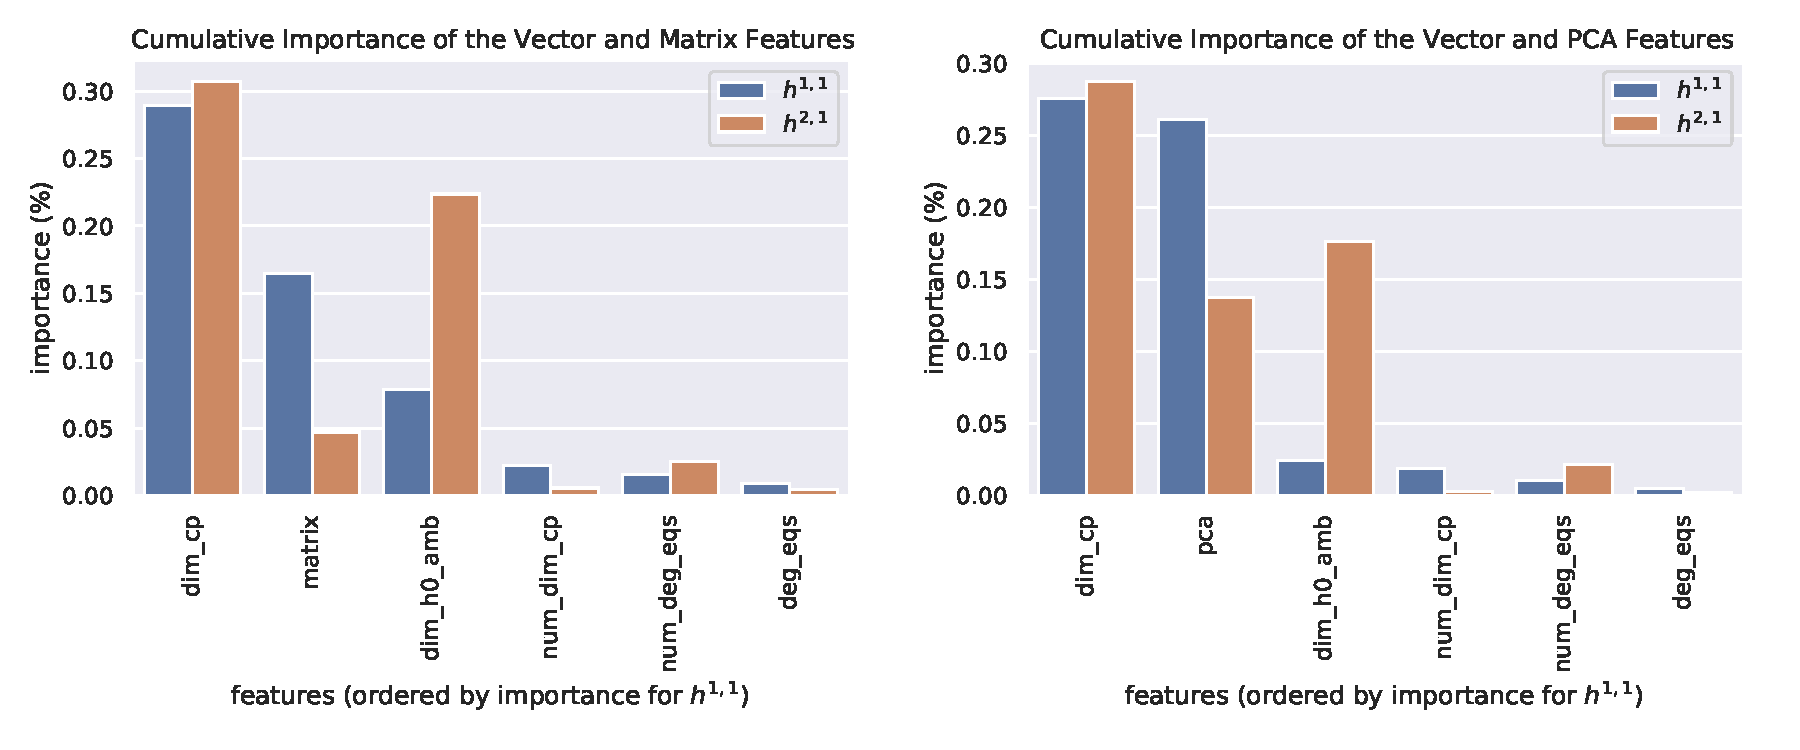
\includegraphics[width=\linewidth]{img/vector-tensor-features_orig}
    \caption{Original dataset}
  \end{subfigure}
  \hfill
  \begin{subfigure}[c]{\linewidth}
    \centering
    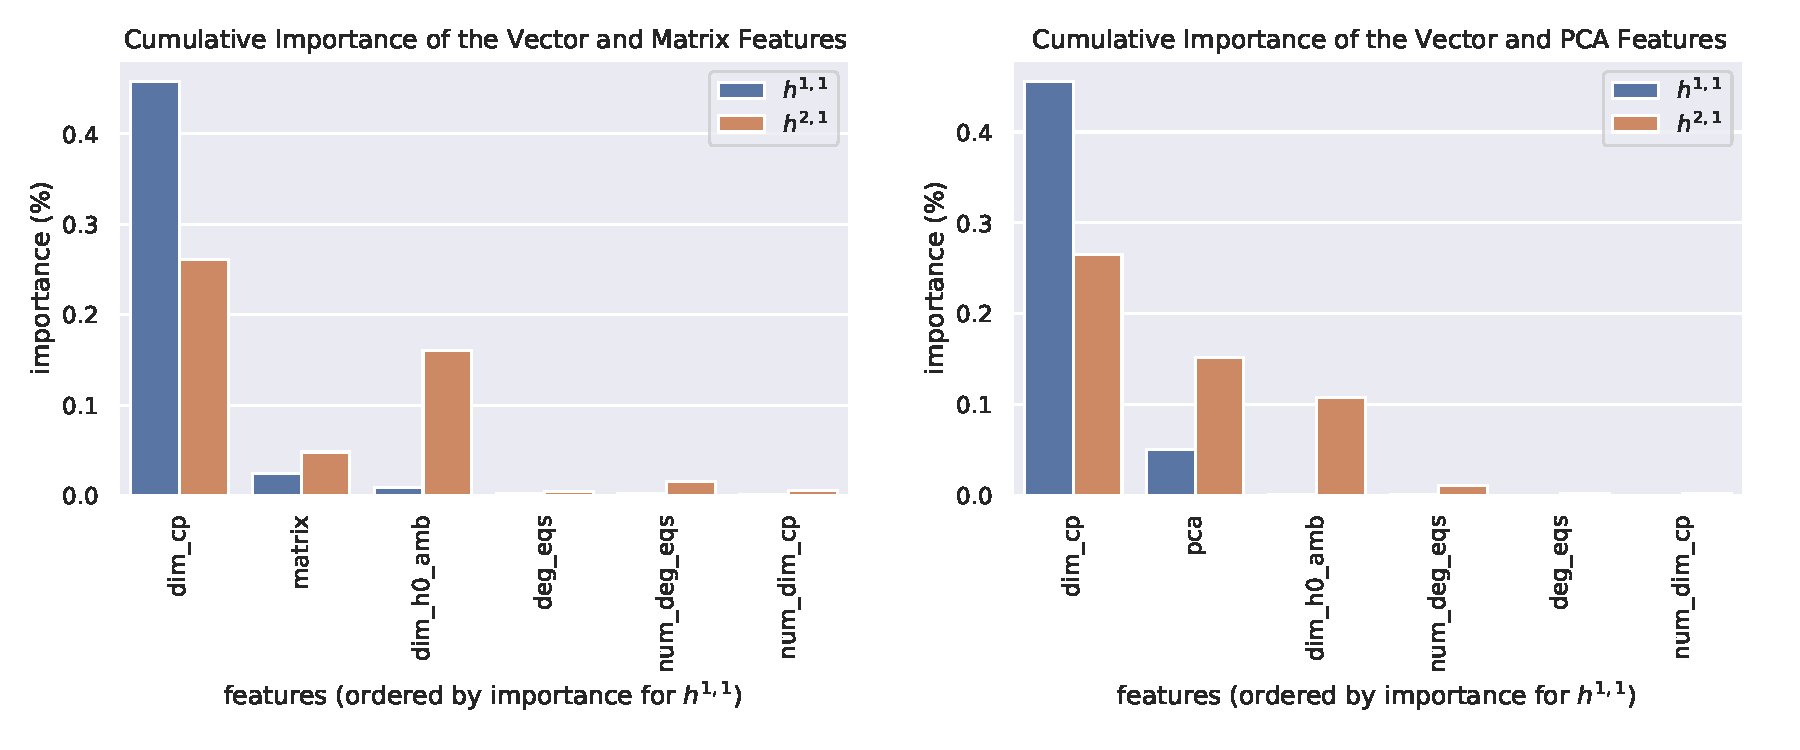
\includegraphics[width=\linewidth]{img/vector-tensor-features_fav}
    \caption{Favourable dataset}
  \end{subfigure}
  \caption{%
    Ranking of the vector features and the configuration matrix (or its \pca).
  }
  \label{fig:eda:tensor}
\end{figure}

In~\Cref{fig:eda:cluster} we show the importance associated to the number of clusters used during the \eda: no matter how many clusters we use, their relevance is definitely marginal compared to all other features used in the variable ranking (scalars, vectors, and the configuration matrix or its \pca) for both datasets.

\begin{figure}[tbp]
  \centering
  \begin{subfigure}[c]{0.45\linewidth}
    \centering
    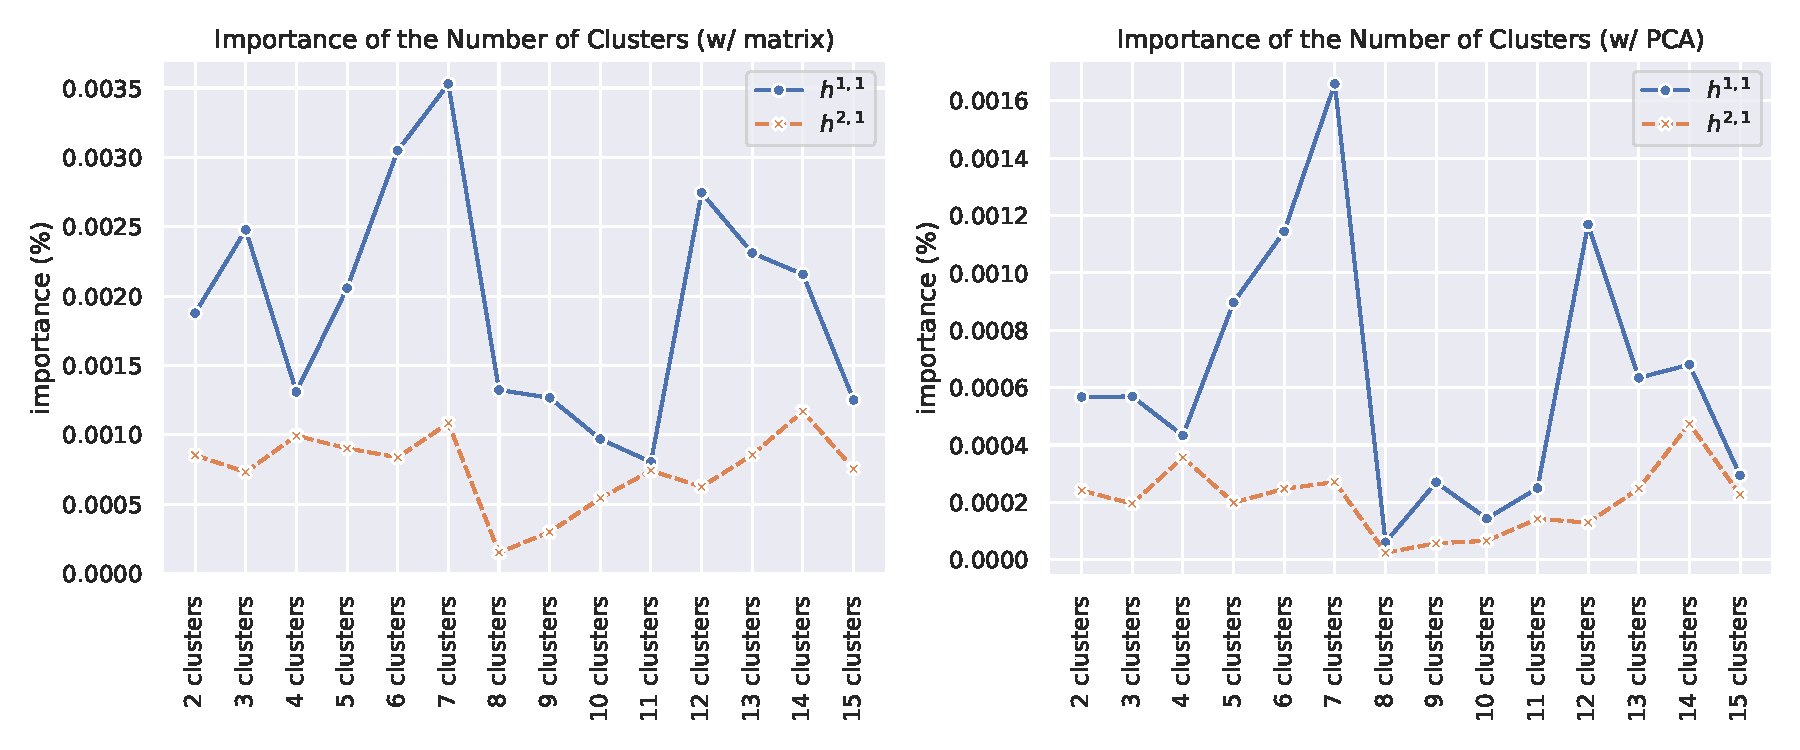
\includegraphics[width=\linewidth, trim={0 0 6in 0}, clip]{img/cluster-features_orig}
    \caption{Original dataset}
  \end{subfigure}
  \hfill
  \begin{subfigure}[c]{0.45\linewidth}
    \centering
    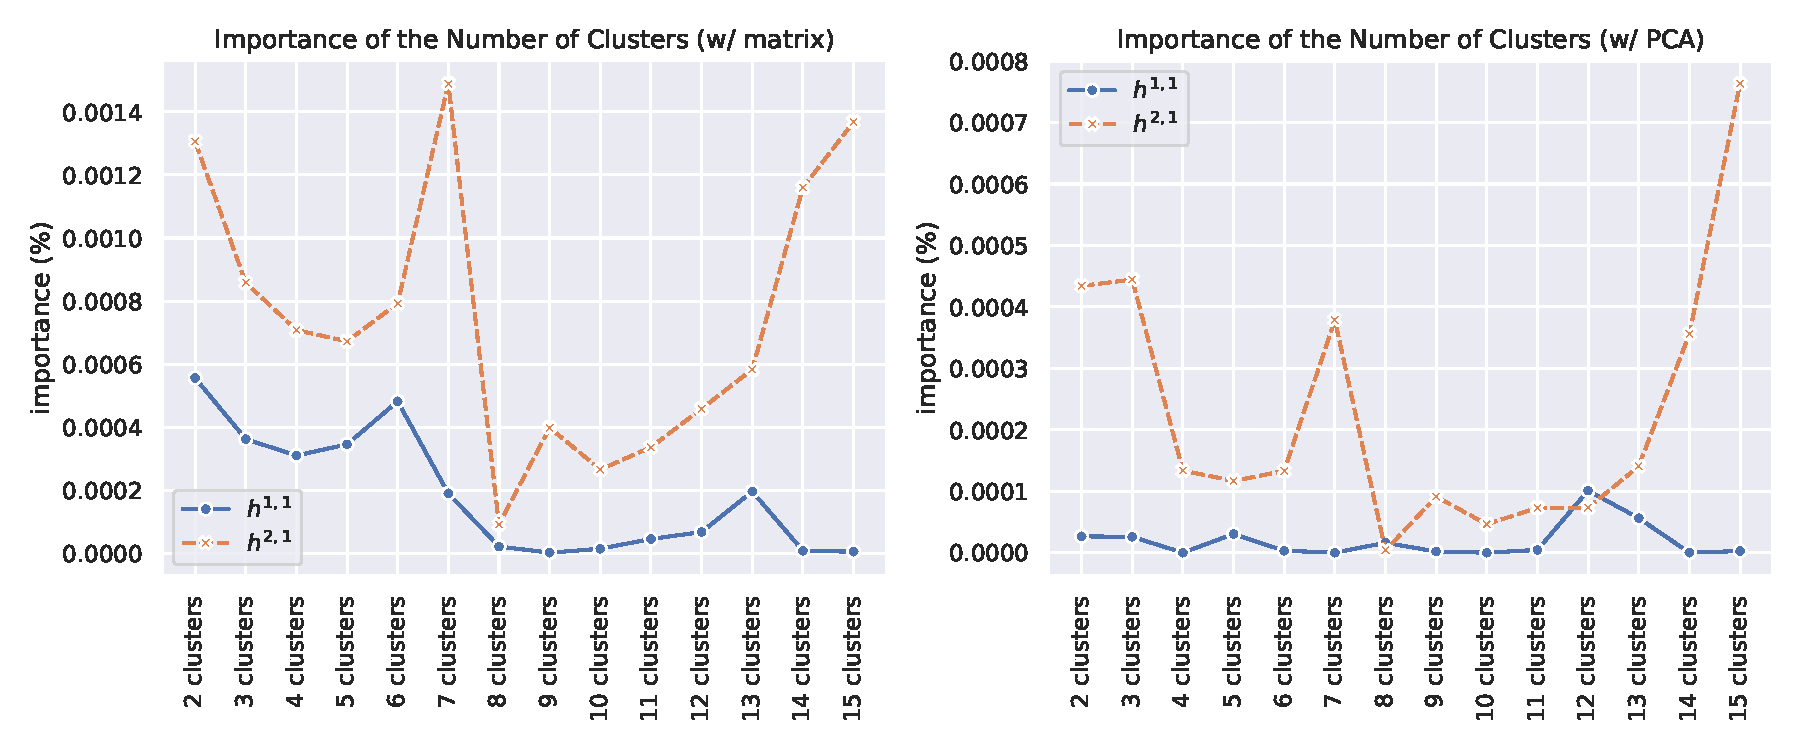
\includegraphics[width=\linewidth, trim={0 0 6in 0}, clip]{img/cluster-features_fav}
    \caption{Favourable dataset}
  \end{subfigure}
  \caption{%
    Incidence of the numbers of clusters on the variable ranking.
  }
  \label{fig:eda:cluster}
\end{figure}

\begin{figure}[tbp]
  \centering
  \begin{subfigure}[c]{\linewidth}
    \centering
    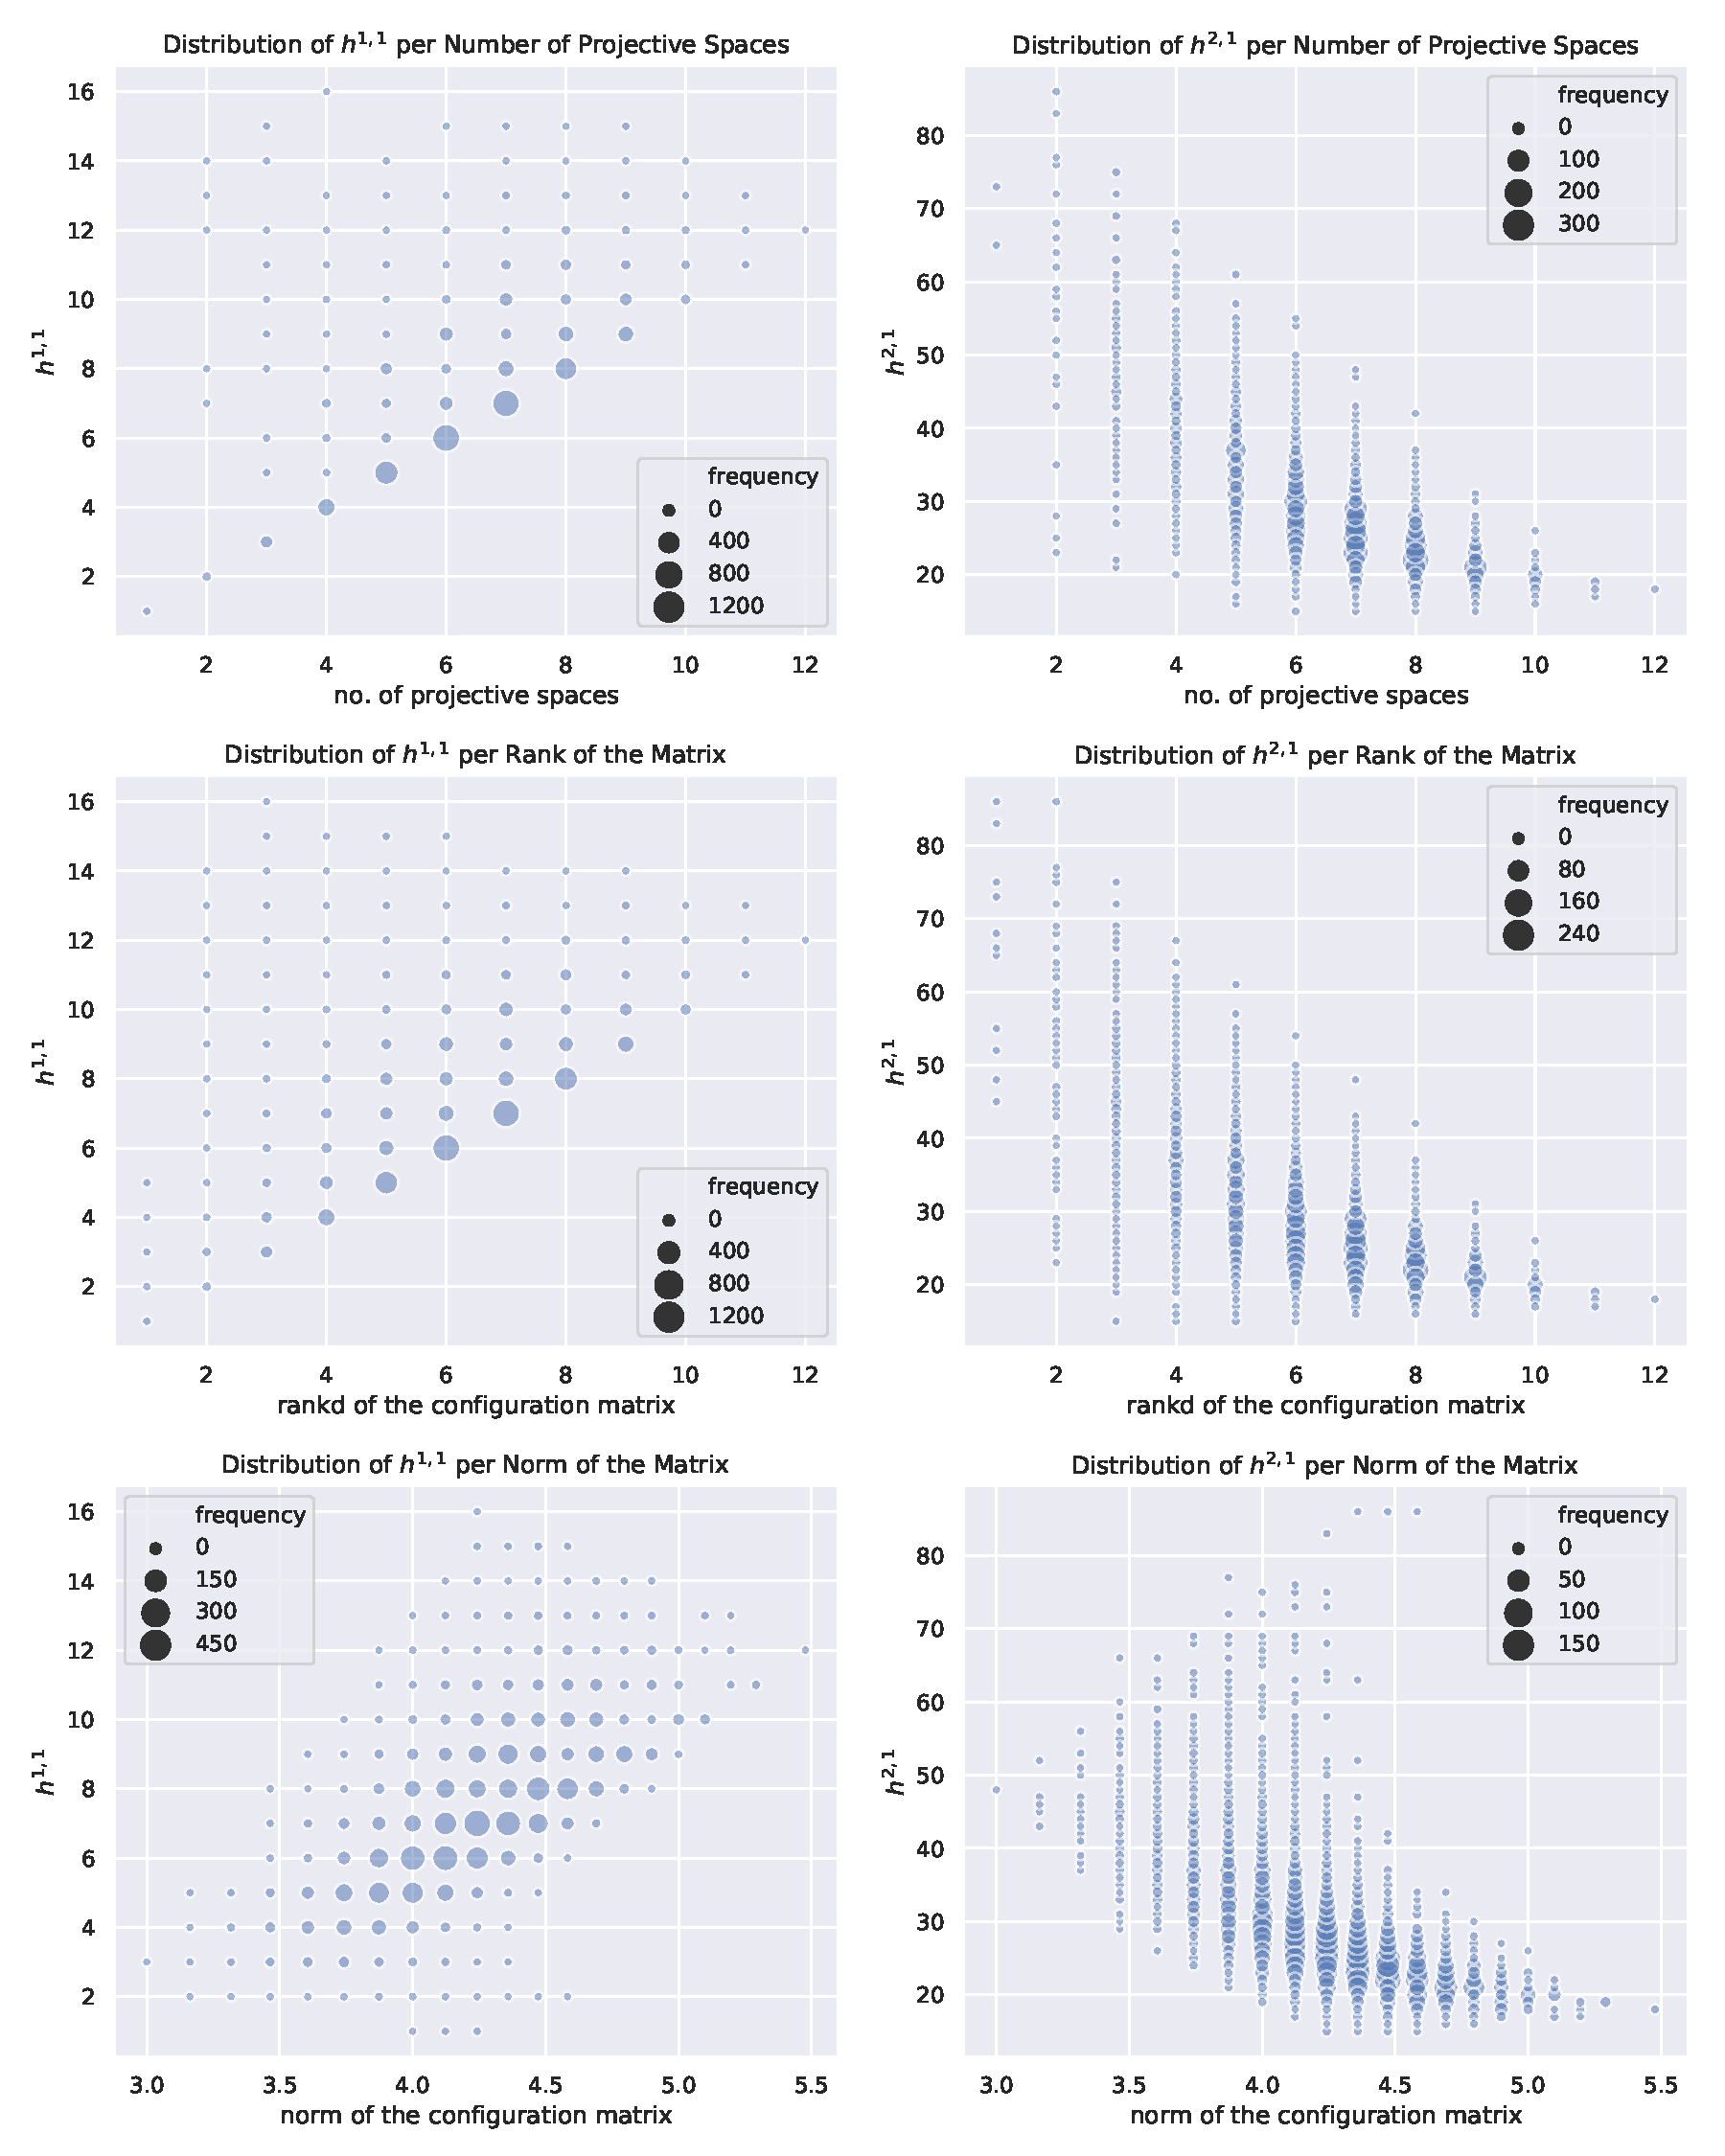
\includegraphics[width=\linewidth, trim={0 10in 0 0}, clip]{img/distr-labels-corr-feat_orig}
    \caption{Original dataset}
  \end{subfigure}
  \begin{subfigure}[c]{\linewidth}
    \centering
    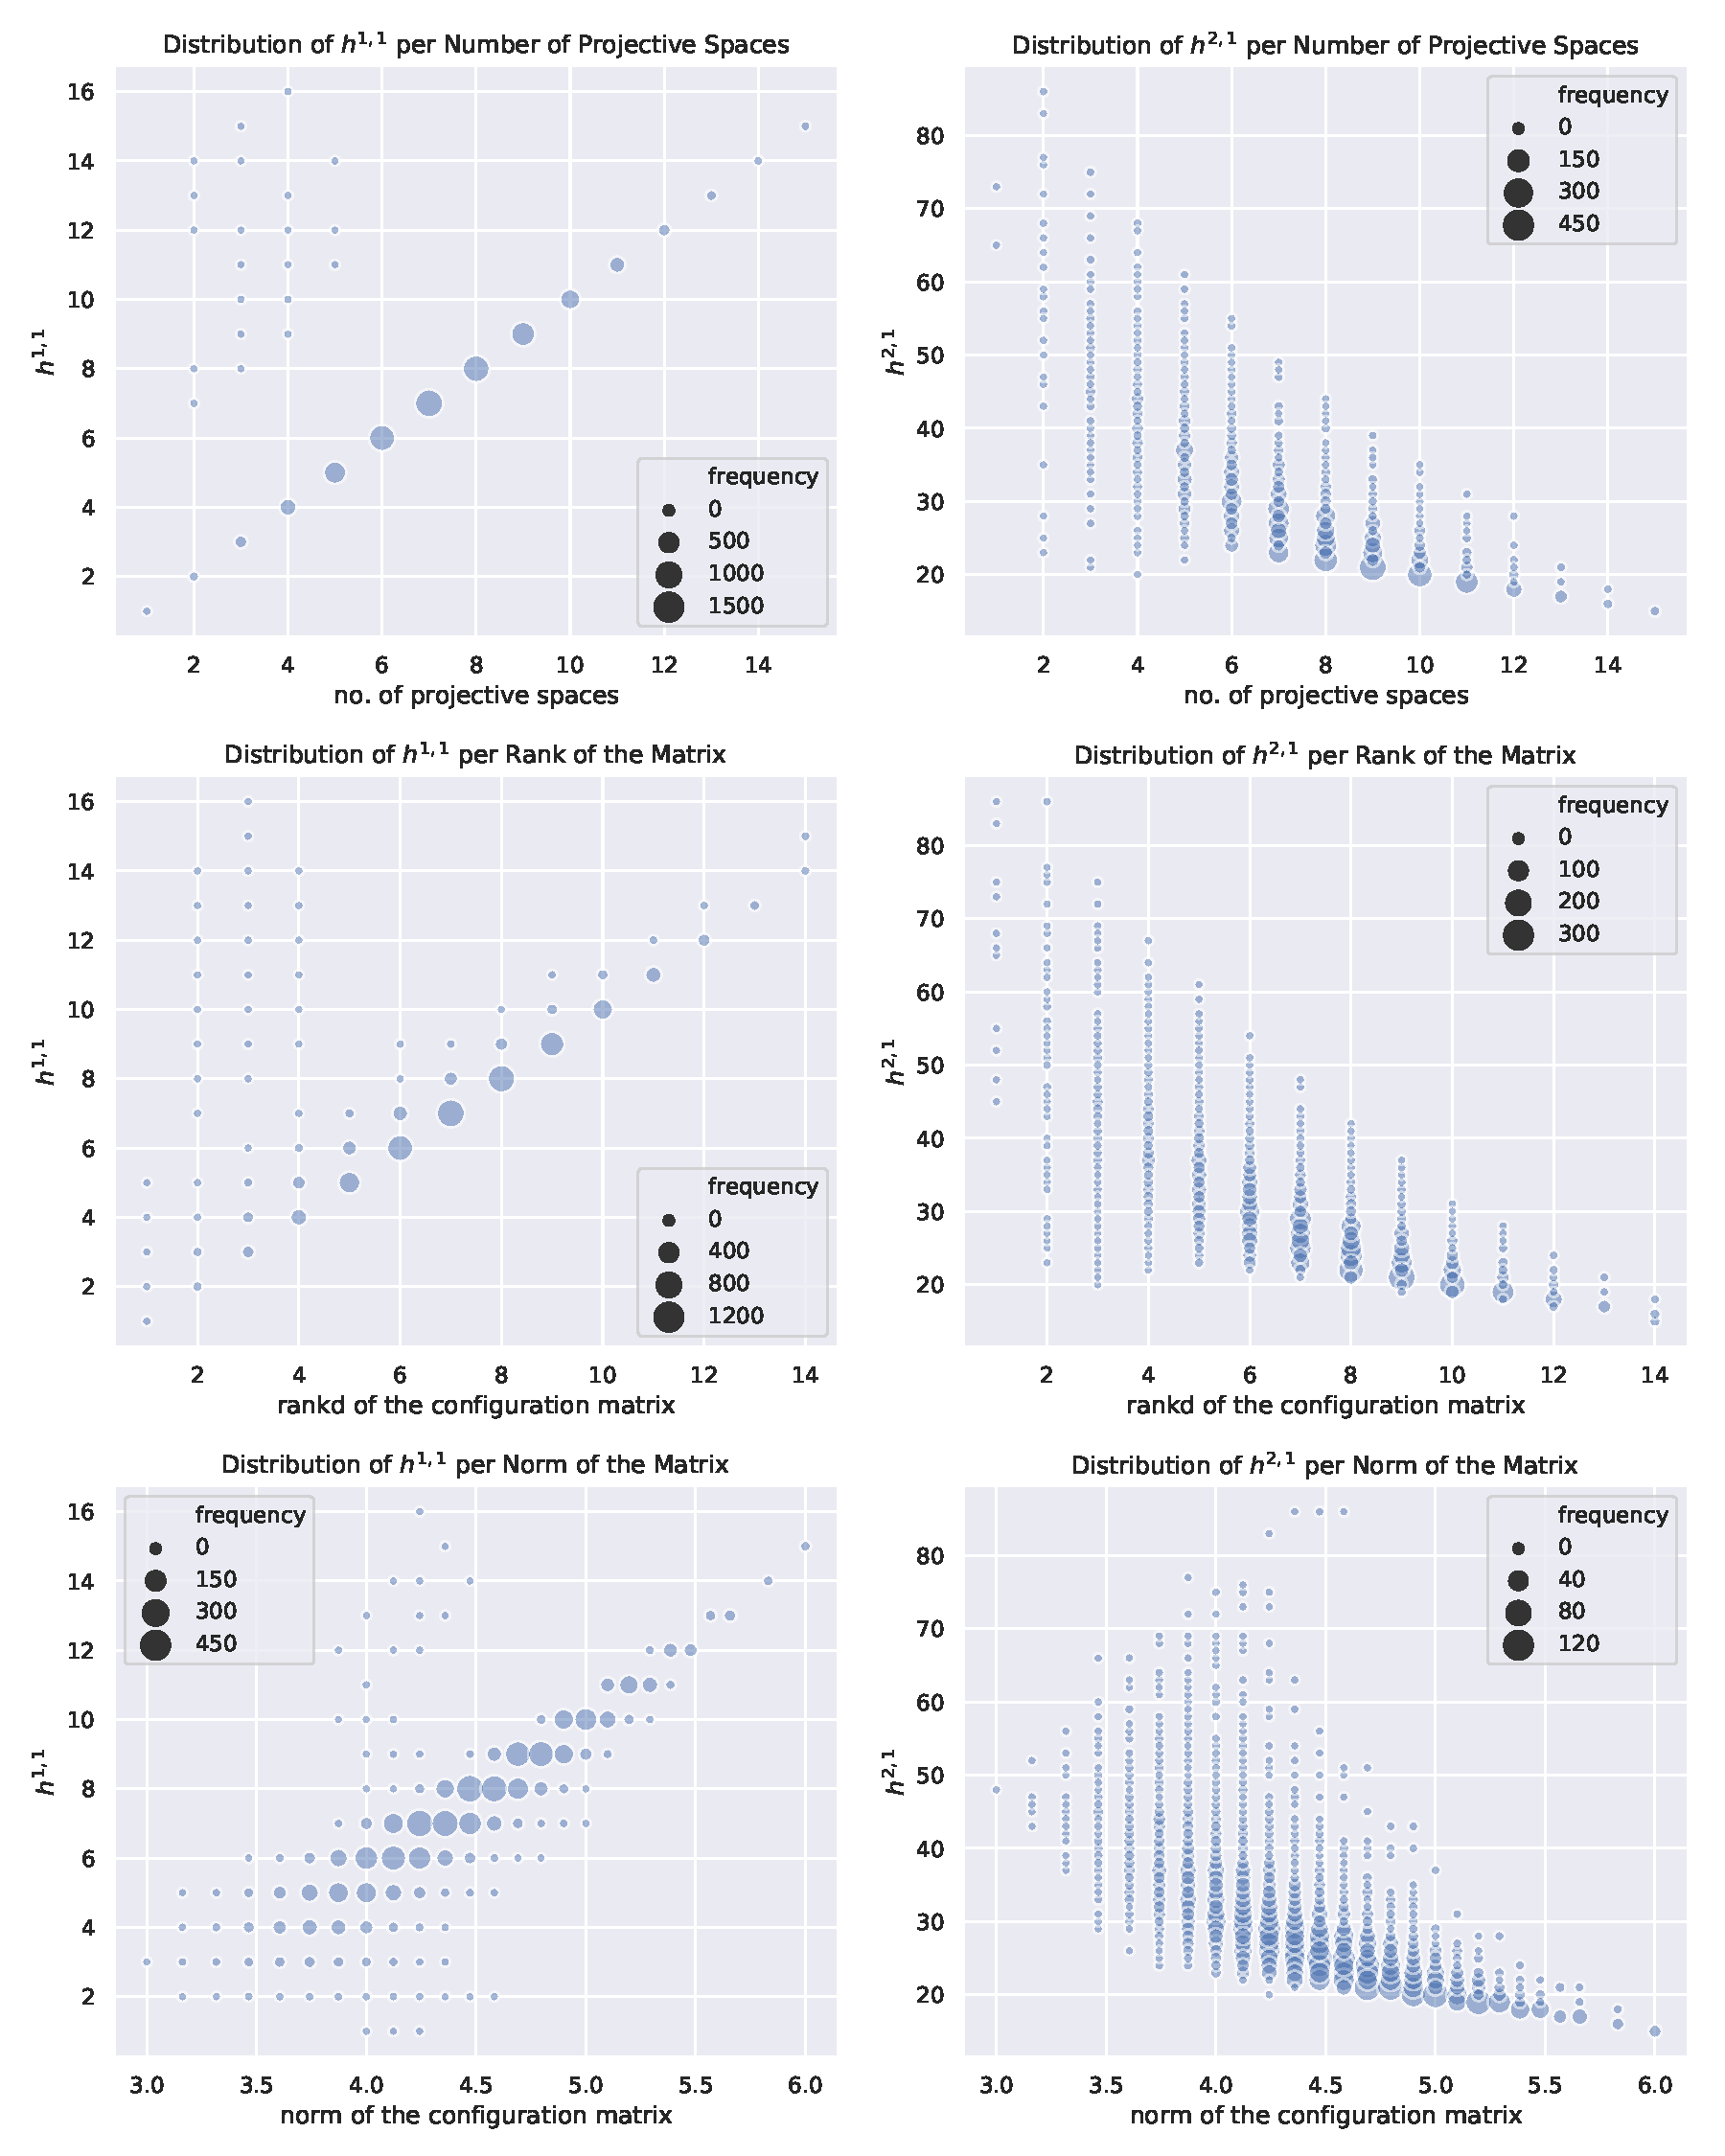
\includegraphics[width=\linewidth, trim={0 10in 0 0}, clip]{img/distr-labels-corr-feat_fav}
    \caption{Favourable dataset}
  \end{subfigure}
  \caption{%
    Distribution of the labels with respect to the number of projective spaces.
  }
  \label{fig:eda:distr}
\end{figure}


\paragraph{Discussion}

It seems therefore that the number of projective spaces plays a relevant role in the determination of \hodge{1}{1} and \hodge{2}{1} as well as the list of dimensions of the projective spaces.
In order to validate this observation, in~\Cref{fig:eda:distr} we present a scatter plot of the Hodge number distributions versus the number of projective spaces: it shows that there is indeed a linear dependence in $m$ for \hodge{1}{1}, especially in the favourable dataset.
In fact the only exceptions to this pattern in the latter case are the manifolds which do not have a favourable embedding~\cite{Anderson:2017:FibrationsCICYThreefolds}.
Hence, a simple data analysis hints naturally towards this mathematical result.

Finally we found other features which may be relevant and are worth to be included in the algorithm: the matrix rank and norm, the list of projective space dimensions and of the associated cohomology dimensions.
However, we want to emphasize one caveat to this analysis: correlations look only for linear relations, and the random forest has not been optimized or could just be not powerful enough to make good predictions.
This means that feature selection just gives a hint but it may be necessary to adapt it to different situations.


\subsubsection{Removing Outliers}
\label{sec:data:eda:outliers}

The Hodge number distributions (see \Cref{fig:data:hist-hodge,fig:data:distr}) display few outliers outside the tail of the main distributions.
Such outliers may negatively impact the learning process and drive down the accuracy: it makes sense to remove them from the training set.
It is easy to see that the \num{22} outlying manifolds with $\hodge{1}{1} = \hodge{2}{1} = 0$ are product spaces, recognisable from their block-diagonal matrix.
We will also remove outliers with $\hodge{1}{1} = 19$ and $\hodge{2}{1} > 86$, which represent $15$ and $2$ samples.
In total this represents $39$ samples, or \SI{0.49}{\percent} of the total data.

To simplify the overall presentation, since the dataset is complete we will mainly focus on the pruned subset of the data obtained by removing outliers, even from the test set.\footnotemark{}
\footnotetext{%
  There is no obligation to use a \ml algorithm to label outliers in the training set.
  It is perfectly fine to decide which data to include or not, even based on targets.
  However, for a real-world application, outliers in the test set should be labeled by some process based only on the input features.
  Flagging possible outliers may improve the predictions by helping the machine understand that such samples require more caution.
}
This implies that Hodge numbers lie in the ranges $1 \le \hodge{1}{1} \le 16$ and $15 \le \hodge{2}{1} \le 86$.
Except when stated otherwise, accuracy is indicated for this pruned dataset.
Obviously the very small percentage of outliers makes the effect of removing them from the test set negligible when stating accuracy.

\begin{figure}[tbp]
  \centering
  \begin{subfigure}[c]{0.45\linewidth}
    \centering
    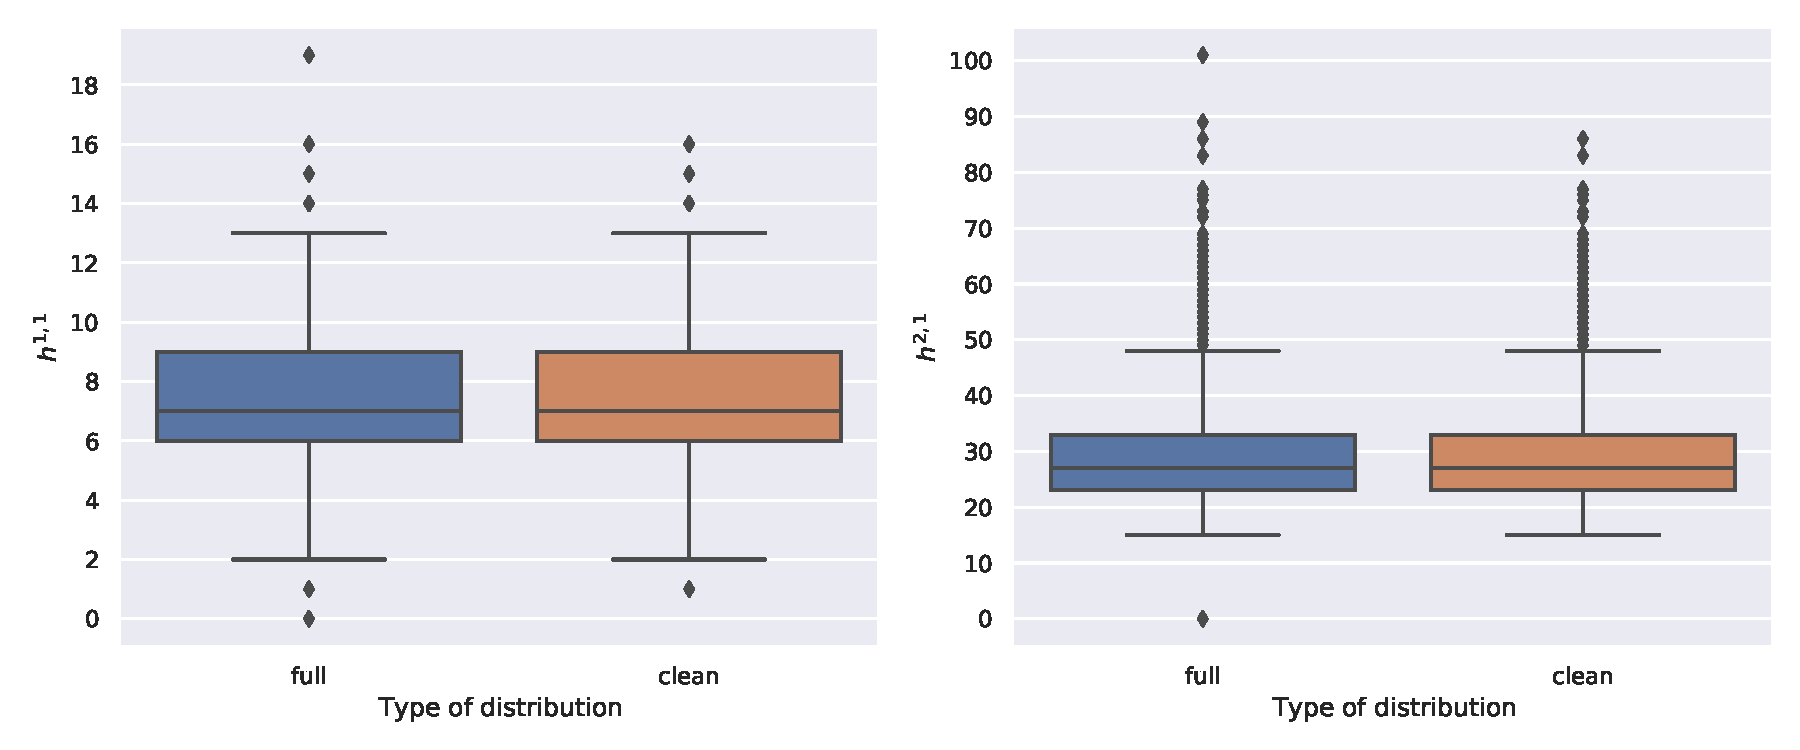
\includegraphics[width=\linewidth, trim={0 0 6in 0}, clip]{img/label-distribution-compare_orig}
    \caption{\hodge{1}{1}}
  \end{subfigure}
  \qquad
  \begin{subfigure}[c]{0.45\linewidth}
    \centering
    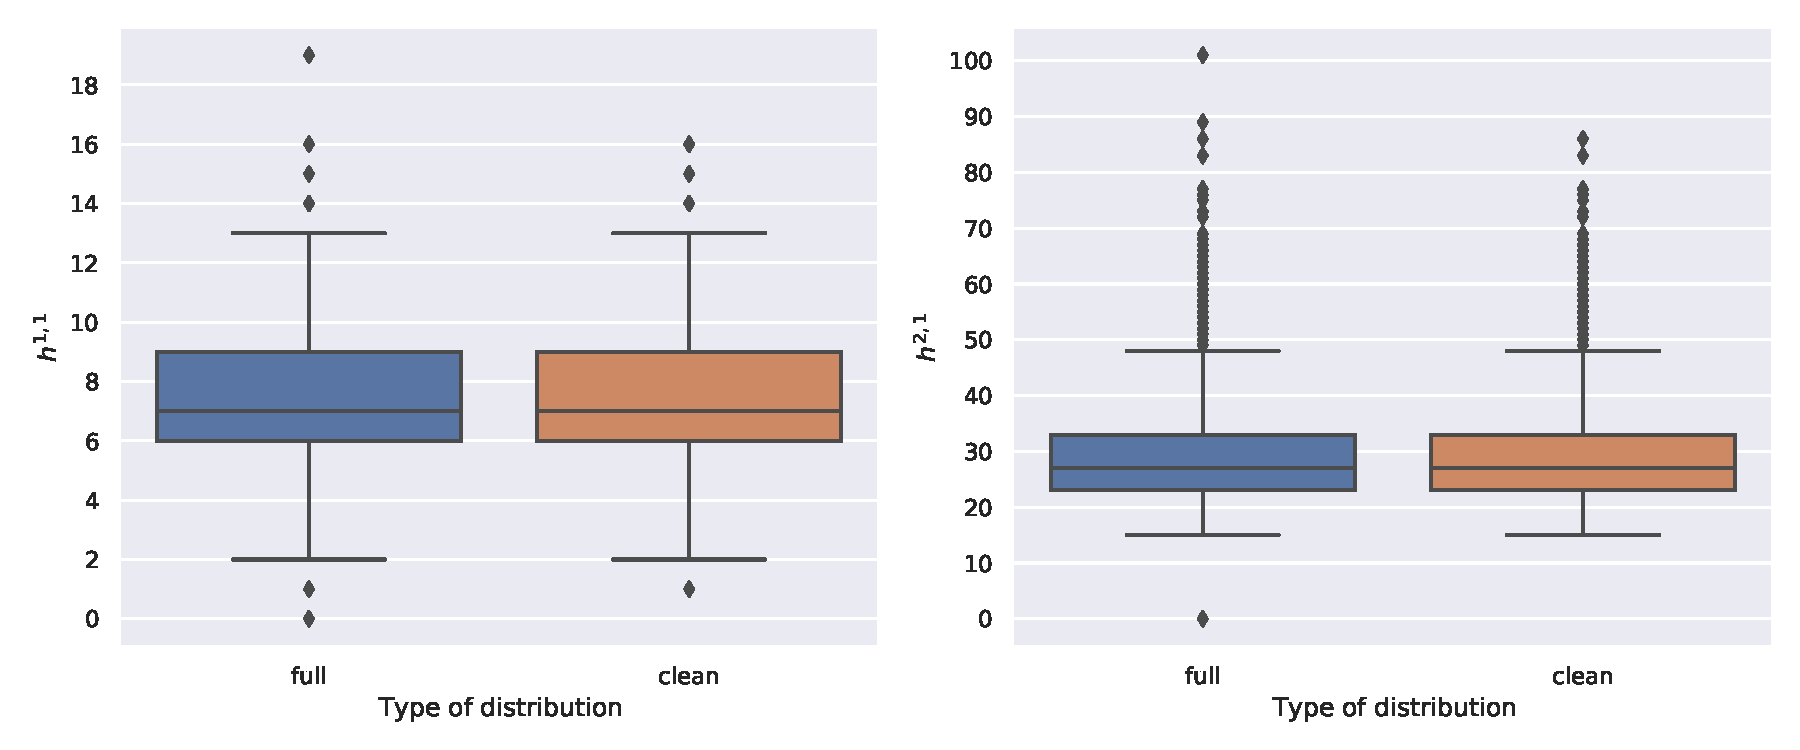
\includegraphics[width=\linewidth, trim={6in 0 0 0}, clip]{img/label-distribution-compare_orig}
    \caption{\hodge{2}{1}}
  \end{subfigure}
  
  \caption{%
    Summary of the statistics for the distributions of both Hodge numbers.
    The coloured box shows the three quartiles of the distributions, with the internal horizontal line corresponding to the median.
    The ``whiskers'' cover the interquartile range, i.e.\ $1.5$ times the distance between the first and third quartiles from the lower and upper limits of the boxes.
    Isolated points show the remaining outliers which we however choose to keep to avoid excessively pruning the dataset.
  }
  \label{fig:data:distr}
\end{figure}


\subsection{Machine Learning Analysis}
\label{sec:ml}

We compare the performances of different \ml algorithms: linear regression, support vector machines (\svm), random forests, gradient boosted trees and (deep) neural networks.
We obtain the best results using deep \emph{convolutional} neural networks.
In fact we present a new neural network architecture, inspired by the Inception model~\cite{Szegedy:2015:GoingDeeperConvolutions, Szegedy:2016:RethinkingInceptionArchitecture, Szegedy:2016:Inceptionv4InceptionresnetImpact} which has been developed in the field of computer vision.
We provide some details on the different algorithms in~\Cref{app:ml-algo} and refer the reader to the literature~\cite{Bengio:2017:DeepLearning, Chollet:2018:DeepLearningPython, Geron:2019:HandsOnMachineLearning, Skiena:2017:DataScienceDesign, Mehta:2019:HighbiasLowvarianceIntroduction, Carleo:2019:MachineLearningPhysical, Ruehle:2020:DataScienceApplications} for more details.


\subsubsection{Feature Extraction}
\label{sec:ml:selection}

In~\Cref{sec:data:eda} the \eda showed that several engineered features are promising for predicting the Hodge numbers.
In what follows we compare the performances of various algorithms using different subsets of features:
\begin{itemize}
  \item only the configuration matrix (no feature engineering);

  \item only the number of projective spaces $m$;

  \item only a subset of engineered features and not the configuration matrix nor its \pca;

  \item a subset of engineered features and the \pca of the matrix.
\end{itemize}

Following the \eda and feature engineering, we finally select the features we use in the analysis by choosing the highest ranked features.
We keep the number of projective spaces (\texttt{num\_cp} in the dataset) and the list of the dimension of the projective spaces (\texttt{dim\_cp}) for both \hodge{1}{1} and \hodge{2}{1}).
We also include the dimension of the cohomology group of the ambient space \texttt{dim\_h0\_amb} but only for \hodge{2}{1}.\footnotemark{}
\footnotetext{%
  Notice that providing different kinds of input features to the algorithm is fine as long as such variables come from the same training set.
  In other words, it is possible to provide different representations of the same set to different algorithms while retaining the same statistical relevance~\cite{Geron:2019:HandsOnMachineLearning, Skiena:2017:DataScienceDesign}.
}


\subsubsection{Analysis Strategy}
\label{sec:ml:strategy}

For the \ml analysis, we split the dataset into training and test sets: we fit the algorithms on the first and then show the predictions on the test set, which will not be touched until the algorithms are ready.


\paragraph{Test split and validation}

The training set is made of \SI{90}{\percent} of the samples for training, which leaves the remaining \SI{10}{\percent} in the test set (i.e.\ $785$ manifolds out of the $7851$ in the set).\footnotemark{}
\footnotetext{%
  Remember that we have removed outliers, see~\Cref{sec:data:eda:outliers}.
  The interested reader can refer to~\cite{Erbin:2020:InceptionNeuralNetwork} where outliers are kept in the test set.
}
For most algorithms, we use \emph{leave-one-out} cross-validation on the training set as evaluation of the algorithm: we subdivide the training set in $9$ subsets, each of them containing \SI{10}{\percent} of the \emph{total} amount of samples, then we train the algorithm on $8$ of them and evaluate it on the $9$th.
We then repeat the procedure changing the evaluation fold until the algorithm has been trained and evaluated on all of them.
The performance measure in validation is given by the average over all the left out folds.
When training neural networks, we will however use a single \emph{holdout validation} set made of \SI{10}{\percent} of the \emph{total} samples.


\paragraph{Predictions and metrics}

Since we are interested in predicting exactly the Hodge numbers, the appropriate metric measuring the success of the predictions is the accuracy (for each Hodge number separately):
\begin{equation}
  \text{accuracy}
  =
  \frac{1}{N} \finitesum{i}{1}{N}
  \delta_{y^{\text{true}\, (i)},\, y^{\text{pred}\, (i)}},
\end{equation}
where $N$ is the number of samples.
In this analysis the accuracy of the predictions on the test set is rounded to the nearest integer.

Since the Hodge numbers are integers the problem of predicting them looks like a classification task.
However, as argued in the introduction, we prefer to use a regression approach.
Indeed regression does not require to specify the data boundaries and allows to extrapolate beyond them, contrary to a classification approach where the categories are fixed at the beginning.\footnotemark{}
\footnotetext{%
  A natural way to transform the problem in a regression task is to \emph{standardise} the Hodge numbers, for example by shifting by the mean value and diving by the standard deviation.
  Under this transformation, the Hodge numbers are mapped to real numbers.
  While standardisation often improves \ml algorithms, we found that the impact was mild or even negative.
}

Most algorithms need a differentiable loss function since the optimisation of parameters (such as neural networks weights) uses some variant of the gradient descent method.
For this reason the accuracy cannot be used and the models are trained by minimisation of the mean squared error (\mse), which is simply the squared $\ell_2$-norm between of the difference between the predictions and the real values.
There will however be also a restricted number of cases in which we will use either the mean absolute error (\mae), which is the $\ell_1$-norm of the same difference, or a weighted linear combination of \mse and \mae (also known as \textit{Huber} loss): we will point them out at the right time.
When predicting both Hodge numbers together, the total loss is the sum of each individual loss with equal weight: \hodge{1}{1} is simpler to learn so it is useful to put emphasis on learning \hodge{2}{1}, but the magnitudes of the latter are higher, such that the associated loss is naturally bigger (since we did not normalise the data).

In general predictions are real numbers: we need to turn them into integers.
In general, rounding to the nearest integer gives the best result, but we found algorithms (such as linear regression) for which flooring to the integer below works better.
The optimal choice of the integer function is found for each algorithm as part of the hyperparameter optimisation described below.
The accuracy is computed after rounding.

Learning curves for salient models are displayed.
They show how the performances of a model improves by using more training data, for fixed hyperparameters.
To obtain it, we train models using from \SI{10}{\percent} to \SI{90}{\percent} of all the data (``training ratio'') and evaluate the accuracy on the remaining data.\footnotemark{}
\footnotetext{%
  Statistics are not provided due to the limitations of our available computational resources, namely a \emph{Thinkpad t470p} laptop with \emph{Intel i7-7700HQ} CPU, \SI{16}{\giga\byte} RAM and \emph{NVidia GeForce 940MX} GPU.
  However, we check manually on few examples that the reported results are typical.
}

To avoid redundant information and to avoid cluttering the paper with graphs, the results for models predicting separately the Hodge numbers for the test set are reported in tables, while the results for the models predicting both numbers together are reported in the learning curves.
For the same reason, the latter are not displayed for the favourable dataset.


\paragraph{Visualisation of the performance}

Complementary to the predictions and the accuracy results, we also provide different visualisations of the performance of the models in the form of univariate plots (histograms) and multivariate distributions (scatter plots).
In fact the usual assumption behind the statistical inference of a distribution is that the difference between the observed data and the predicted values can be modelled by a random variable called \textit{residual}~\cite{Lista:2017:StatisticalMethodsData,Caffo::DataScienceSpecialization}.\footnotemark{}
\footnotetext{%
  The difference between the non observable \textit{true} value of the model and the observed data is known as \textit{statistical error}.
  The difference between residuals and errors is subtle but the two definitions have different interpretations in the context of the regression analysis: in a sense, residuals are an estimate of the errors.
}
As such we expect that its values can be sampled from a normal distribution with a constant variance (i.e.\ constant width), since it should not depend on specific observations, and centered around zero, since the regression algorithm tries to minimise the squared difference between observed and predicted values.
Histograms of the residual errors should therefore exhibit such properties graphically.
Another interesting kind of visual realisation of the residuals is to show their distribution against the variables used for the regression model: in the case of a simple regression model in one variable, it is customary to plot the residuals as a function of the independent variable, but in a multivariable regression analysis (such as the case at hand) the choice usually falls on the values predicted by the fit (not the observed data).
We shall therefore plot the residuals as functions of the predicted values.\footnotemark{}
\footnotetext{
  We will use the same strategy also for the fit using just the number of projective spaces in order to provide a way to compare the plots across different models.
}
Given the assumption of the random distribution of the residuals, they should not present strong correlations with the predictions and should not exhibit trends.
In general the presence of correlated residuals is an indication of an incomplete or incorrect model which cannot explain the variance of the predicted data, meaning that the model is either not suitable for predictions or that we should add information (i.e.\ add features) to it.


\paragraph{Hyperparameter optimisation}

One of the key steps in a \ml analysis is the optimisation of the \emph{hyperparameters} of the algorithm.
These are internal parameters of each estimator (such as the number of trees in a random forest or the amount of regularisation in a linear model): they are not modified during the training of the model, but they directly influence the process in terms of performance and outcome.

Hyperparameter optimisation is performed by training many models with different choices of their values.
We then keep the values best performing according to some metric on the validation set(s).\footnotemark{}
\footnotetext{%
  Notice the importance of having a validation set separate from the test set: we must avoid adapting the algorithm to the same set we use for the predictions or the generalisation capabilities of the algorithm will suffer.
}
As it does not need to be differentiable we use the accuracy as a scoring function to evaluate the models.
There is however a subtle issue because it is not clear how to combine the accuracy of \hodge{1}{1} and \hodge{2}{1} to get a single metric.
For this reason we perform the analysis on both Hodge numbers separately.
Then we can design a single model computing both Hodge numbers simultaneously by making a compromise by hand between the hyperparameters found for the two models computing the Hodge numbers separately.
The optimisation is implemented using the API in \texttt{scikit-learn}, using the function \texttt{metrics.make\_scorer} and the accuracy as a custom scoring function.

There are several approaches to perform this search automatically, in particular: grid search, random search, genetic evolution, and Bayes optimisation.
Grid and random search are natively implemented in \texttt{scikit-learn}.
The first takes a list of possible discrete values of the hyperparameters and will evaluate the algorithm over all possible combinations.
The second samples the values in both discrete sets and continuous intervals according to some probability distribution, repeating the process a fixed number of times.
The grid search method is particularly useful for discrete hyperparameters, less refined searches or for a small number of combinations, while the second method can be used to explore the hyperparameter space on a larger scale~\cite{Bergstra:2012:RandomSearchHyperparameter}.
Genetic algorithms are based on improving the choice of hyperparameters over \emph{generations} that successively select only the most promising values: in general they require a lot of tuning and are easily influenced by the fact that the replication process can also lead to worse results totally at random~\cite{Rudolph:1994:ConvergenceAnalysisCanonical}.
They are however effective when dealing with very deep or complex neural networks.
Bayes optimisation~\cite{Snoek:2012:PracticalBayesianOptimization, Shahriari:2015:TakingHumanOut} is a very well established mathematical procedure to find the stationary points of a function without knowing its analytical form~\cite{Mockus:1975:BayesianMethodsSeeking}.
It relies on assigning a \emph{prior} probability to a given parameter and then multiply it by the probability distribution (or \emph{likelihood}) of the scoring function to compute the probability of finding a better results given a set of hyperparameters.
This has proven to be very effective in our case and we adopted this solution as it does not require fine tuning and leads to better results for models which are not deep neural networks.
We choose to use \texttt{scikit-optimize}~\cite{Head:2020:ScikitoptimizeScikitoptimize} whose method \texttt{BayesSearchCV} has a very well implemented Python interface compatible with \texttt{scikit-learn}.
We will in general perform $50$ iterations of the Bayes search algorithm, unless otherwise specified.


\subsection{Linear Models}

Linear models attempt to describe the labels as a linear combinations of the input features while keeping the coefficients at $\order{1}$ (see \Cref{sec:app:linreg}).
However non-linearity can still be introduced by engineering features which are non-linear in terms of the original data.\footnotemark{}
\footnotetext{%
  In general \emph{linear model} is used to indicate that the coefficients $\beta$ of the features appear linearly in the expression of the prediction of the $i$-th label:
  \begin{equation*}
    y^{\text{pred}\, (i)}
    =
    \beta^{(i)}_0
    +
    \beta^{(i)}_1 x^{(i)}_1
    +
    \dots
    +
    \beta^{(i)}_F x^{(i)}_F
    =
    \finitesum{j}{0}{F} \beta^{(i)}_j x^{(i)}_j,
  \end{equation*}
  where $m$ is the number of independent variables and $x^{(i)}_0 = 1$ (i.e.\ $\beta^{(i)}_0$ is the intercept of the model and represents the value of the label without the contribution of any of the features).
  In other words, $\beta^{(i)}_j$ are used with unit exponent only once per model.
}

From the results of \Cref{sec:data:eda}, we made a hypothesis on the linear dependence of \hodge{1}{1} on the number of projective spaces $m$.
As a first approach, we can try to fit a linear model to the data as a baseline computation and to test whether there is actual linear correlation between the two quantities.
We will consider different linear models including their regularised versions.


\paragraph{Parameters}

The linear regression is performed with the class \texttt{linear\_model.ElasticNet} in \texttt{scikit-learn}.
The hyperparameters involved in this case are: the amount of regularisation $\alpha$, the relative ratio (\texttt{l1\_ratio}) between the $\ell_1$ and $\ell_2$ regularization losses, and the fit of the intercept.
By performing the hyperparameter optimisation we found that $\ell_2$ regularization has a minor impact and can be removed, which corresponds to setting the relative ratio to $1$ (this is equivalent to using \texttt{linear\_model.Lasso}).
In \Cref{tab:hyp:lin} we show the choices of the hyperparameters for the different models we built using the $\ell_1$ regularised linear regression.

For the original dataset, we floored the predictions to the integers below, while in the favourable we rounded to the next integer.
This choice for the original dataset makes sense: the majority of the samples lie on the line $\hodge{1}{1} = m$, but there are still many samples with $\hodge{1}{1} > m$ (see \Cref{fig:eda:distr}).
As a consequence the \ml prediction pulls the line up which can only damage the accuracy.
Choosing the floor function is a way to counteract this effect.
Note that accuracy for \hodge{2}{1} is only slightly affected by the choice of rounding, so we just choose the same one as \hodge{1}{1} for simplification.


\begin{table}[tbp]
\centering
\resizebox{\linewidth}{!}{%
\begin{tabular}{@{}lccccccccc@{}}
\toprule
                                                          &           & \multicolumn{2}{c}{\textbf{matrix}}         & \multicolumn{2}{c}{\textbf{num\_cp}} & \multicolumn{2}{c}{\textbf{eng. feat.}}     & \multicolumn{2}{c}{\textbf{PCA}}            \\ \midrule
                                                          &           & \textit{old}         & \textit{fav.}        & \textit{old}  & \textit{fav.}        & \textit{old}         & \textit{fav.}        & \textit{old}         & \textit{fav.}        \\ \midrule
\multirow{2}{*}{$\alpha$}                                 & \hodge{1}{1} & $2.0 \times 10^{-6}$ & $3.0 \times 10^{-5}$ & 0.10          & $2.0 \times 10^{-6}$ & 0.05                 & 0.05                 & 0.07                 & 0.08                 \\
                                                          & \hodge{2}{1} & $1.0 \times 10^{-6}$ & $1.0 \times 10^{-5}$ & 0.1           & $1.0 \times 10^{-6}$ & $3.0 \times 10^{-4}$ & $1.2 \times 10^{-3}$ & $2.0 \times 10^{-6}$ & $1.2 \times 10^{-3}$ \\ \midrule
\multirow{2}{*}{\texttt{fit\_intercept}} & \hodge{1}{1} & False                & False                & True          & False                & True                 & True                 & False                & True                 \\
                                                          & \hodge{2}{1} & True                 & True                 & True          & True                 & True                 & False                & True                 & False                \\ \midrule
\multirow{2}{*}{\texttt{normalise}}      & \hodge{1}{1} & ---                  & ---                  & False         & ---                  & False                & False                & ---                  & False                \\
                                                          & \hodge{2}{1} & False                & True                 & False         & False                & False                & ---                  & True                 & ---                  \\ \bottomrule
\end{tabular}%
}
\caption{%
  Hyperparameter choices of the $\ell_1$ regression model used.
  In addition to the known hyperparameters $\alpha$ and \texttt{fit\_intercept}, we also include the \texttt{normalise} parameter which indicates whether the samples have been centered and scaled by their $\ell_2$ norm before the fit: it is ignored when the intercept is ignored.
}
\label{tab:hyp:lin}
\end{table}


\paragraph{Results}

In~\Cref{tab:res:lin} we show the accuracy for the best hyperparameters.
For \hodge{1}{1}, the most precise predictions are given by the number of projective spaces which actually confirms the hypothesis of a strong linear dependence of \hodge{1}{1} on the number of projective spaces.
In fact this gives close to \SI{100}{\percent} accuracy for the favourable dataset which shows that there is no need for more advanced \ml algorithms.
Moreover adding more engineered features \emph{decreases} the accuracy in most cases where regularization is not appropriate.
The accuracy for \hodge{2}{1} remains low but including engineered features definitely improves it.

In~\Cref{fig:res:lin} we show the plots of the residual errors of the model on the original dataset.
For the $\ell_1$ regularised linear model, the univariate plots show that the errors seem to follow normal distributions peaked at $0$ as they generally should: in the case of \hodge{1}{1}, the width is also quite contained.
The scatter plots instead show that in general there is no correlation between a particular sector of the predictions and the error made by the model, thus the variance of the residuals is in general randomly distributed over the predictions.
Only the case of the fit of the number of projective spaces seems to show a slight correlation for \hodge{2}{1}, signalling that the model using only one feature might be actually incomplete: in fact it is better to include also other engineered features.

The learning curves in~\Cref{fig:lc:lin} show that the model underfits.
We also notice that the models are only marginally affected by the number of samples used for training.
In particular this provides a very strong baseline for \hodge{1}{1}.
For comparison, we also give the learning curve for the favourable dataset in~\Cref{fig:lc:lin-fav}: this shows that a linear regression is completely sufficient to determine \hodge{1}{1} in that case.

\begin{table}[tbp]
  \centering
  \begin{tabular}{@{}cccccc@{}}
    \toprule
                            &           & \textbf{matrix} & \textbf{num\_cp} & \textbf{eng. feat.} & \textbf{PCA} \\ \midrule
      \multirow{2}{*}
      {\emph{original}}   & \hodge{1}{1} & \SI{51}{\percent}            & \SI{63}{\percent}             & \SI{63}{\percent}                & \SI{64}{\percent}         \\
                          & \hodge{2}{1} & \SI{11}{\percent}            & \SI{8}{\percent}              & \SI{21}{\percent}                & \SI{21}{\percent}         \\ \midrule
      \multirow{2}{*}
      {\emph{favourable}} & \hodge{1}{1} & \SI{95}{\percent}            & \SI{100}{\percent}            & \SI{100}{\percent}               & \SI{100}{\percent}        \\
                          & \hodge{2}{1} & \SI{14}{\percent}            & \SI{15}{\percent}             & \SI{19}{\percent}                & \SI{19}{\percent}         \\ \bottomrule
  \end{tabular}
  \caption{%
    Best accuracy of the linear model using $\ell_1$ regularisation on the test split.
  }
  \label{tab:res:lin}
\end{table}

\begin{figure}[tbp]
  \centering
  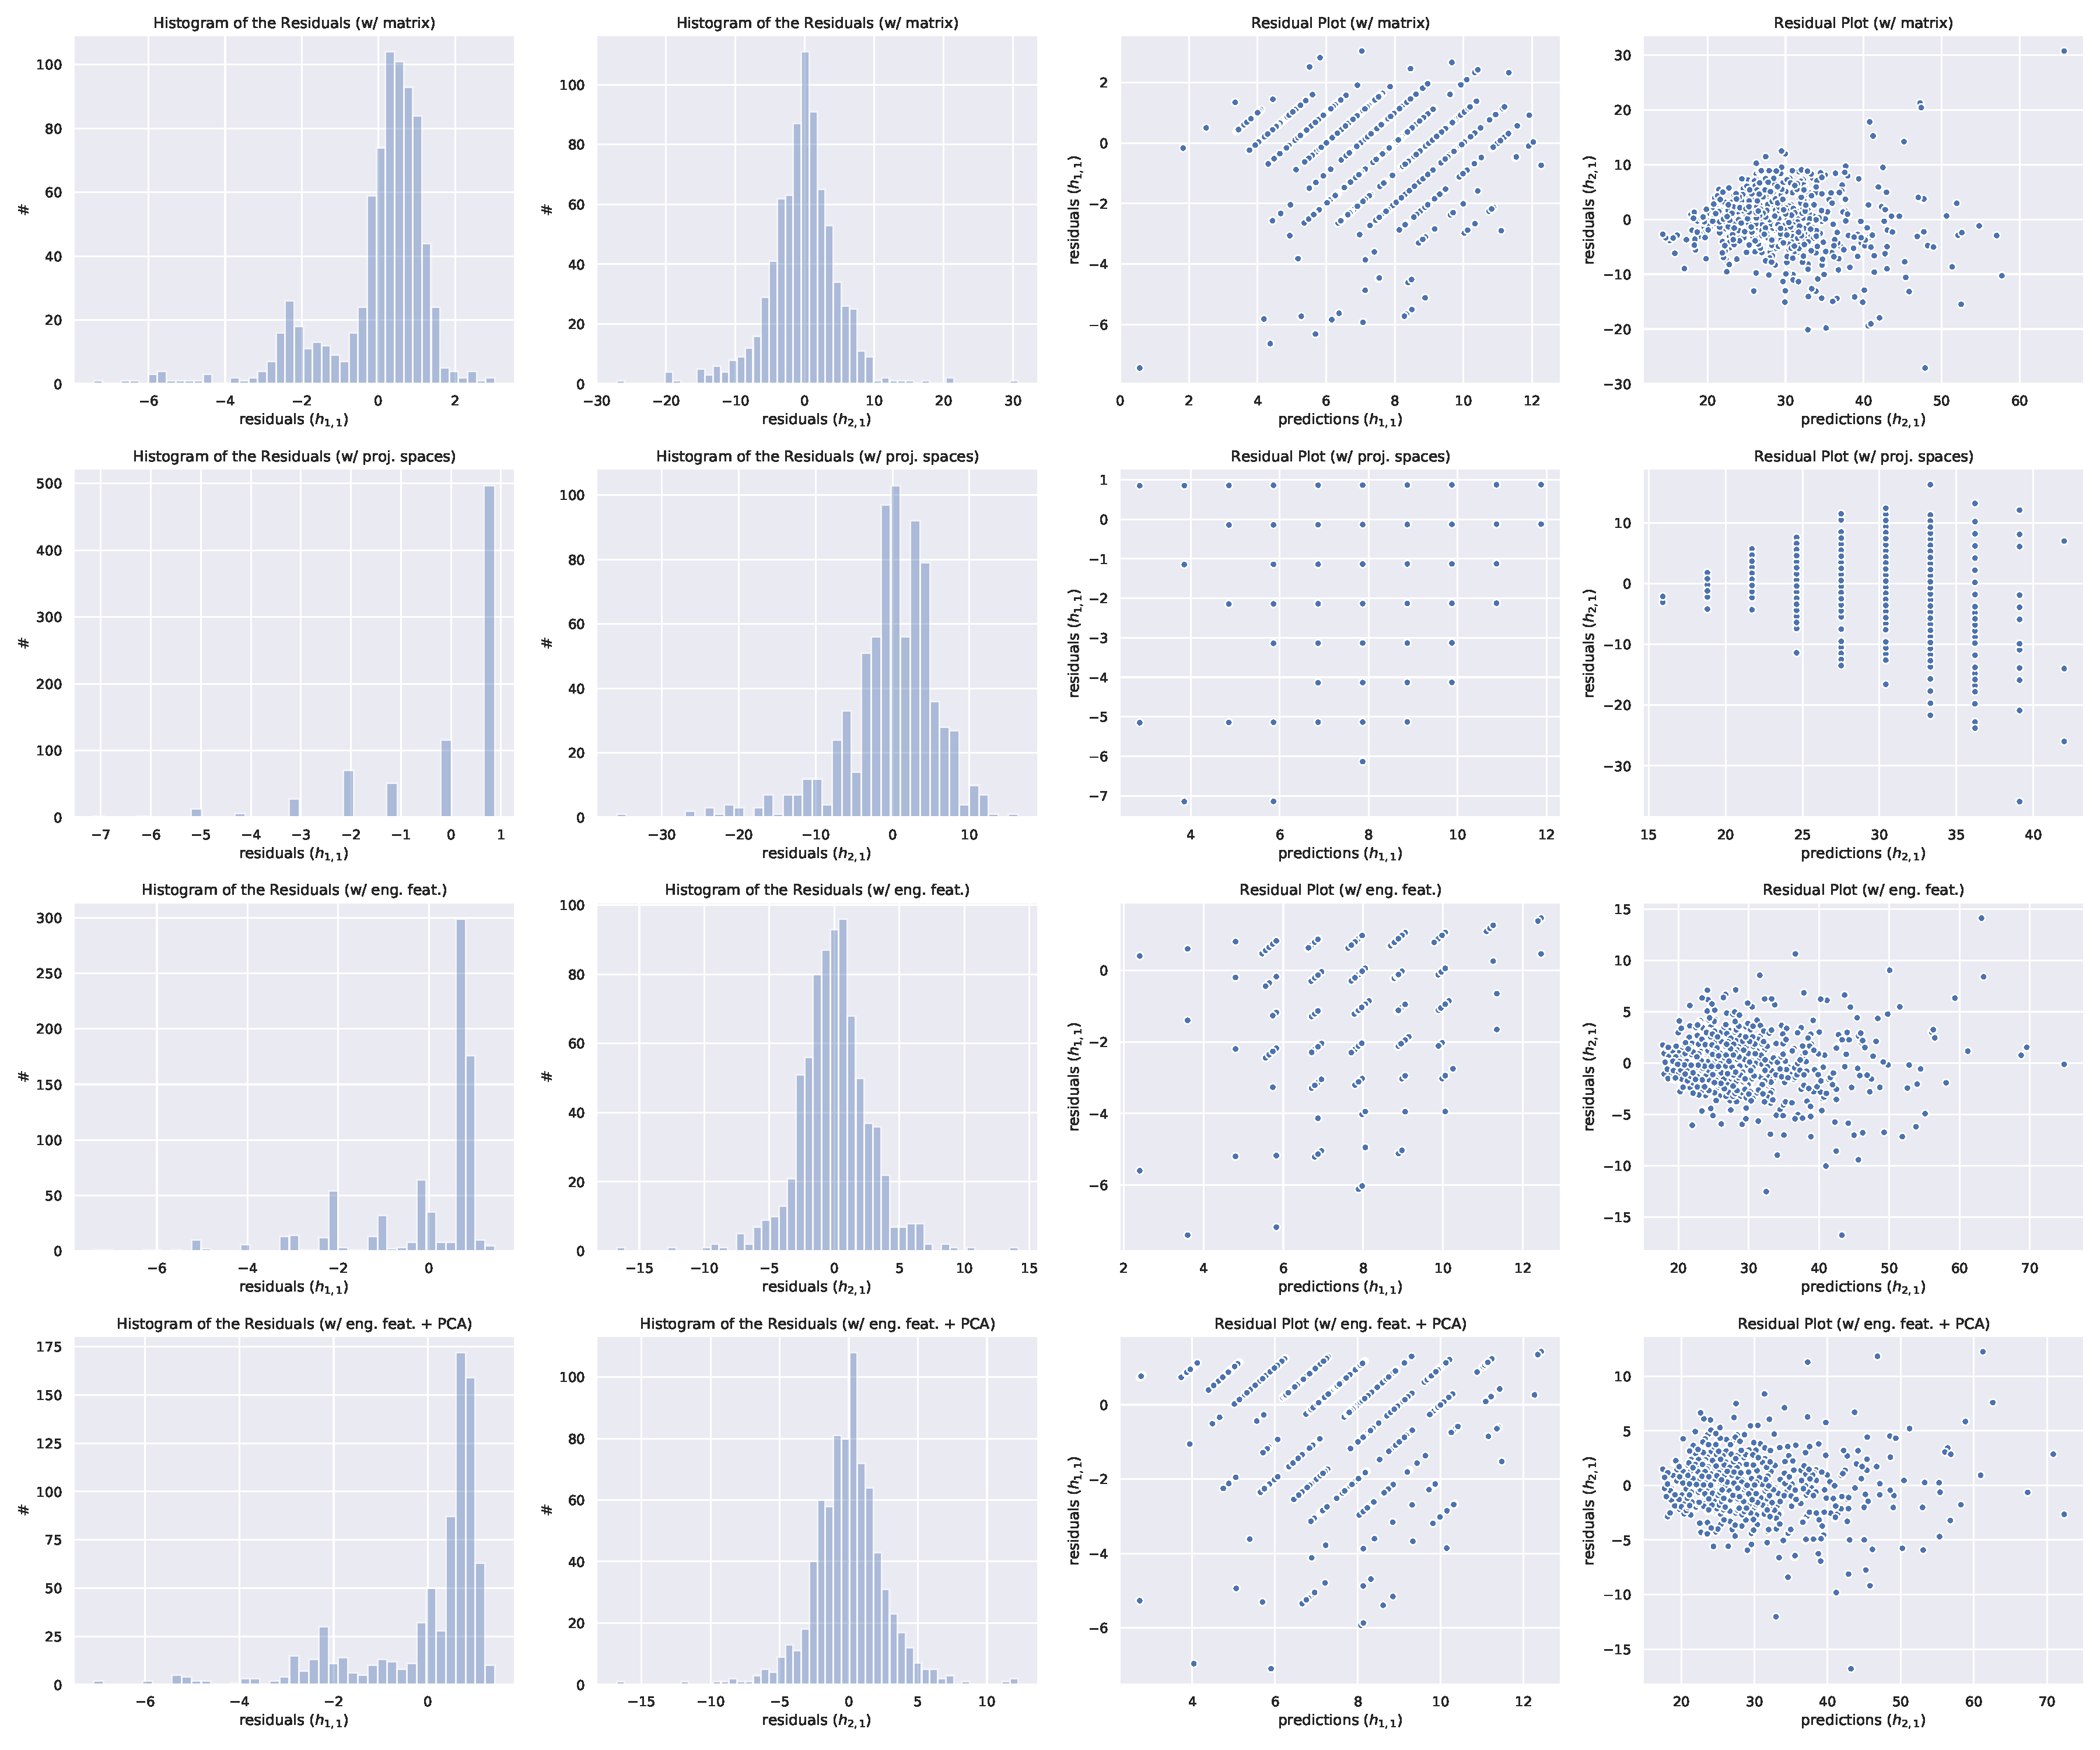
\includegraphics[width=\linewidth]{img/lss_reg_orig}
  \caption{%
    Plots of the residual error for the $\ell_1$ regularised linear model: rows show the different scenarios (fit with only the matrix, with only the number of projective spaces, with the engineered features, with the engineered features and the \pca).
    Plots refer to the test split of the original dataset.
  }
  \label{fig:res:lin}
\end{figure}

\begin{figure}[tbp]
  \centering
  \begin{subfigure}[c]{0.45\linewidth}
    \centering
    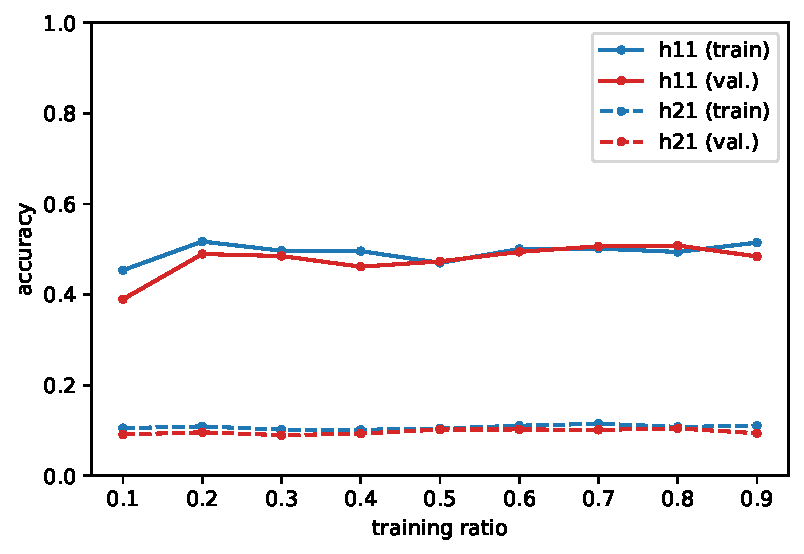
\includegraphics[width=\linewidth]{img/linreg_learning_curve_matrix_outliers}
    \caption{input: \texttt{matrix}, $\alpha = \num{2e-4}$}
  \end{subfigure}
  \hfill
  \begin{subfigure}[c]{0.45\linewidth}
    \centering
    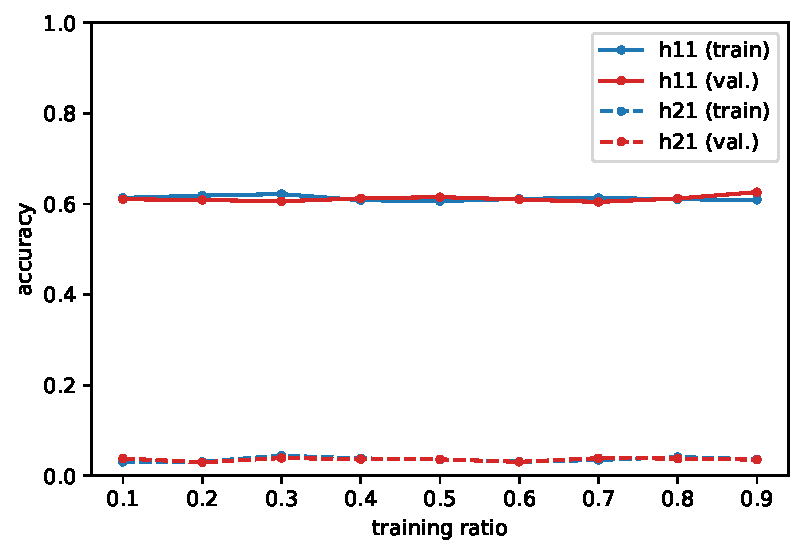
\includegraphics[width=\linewidth]{img/linreg_learning_curve_num_cp_outliers}
    \caption{input: \texttt{num\_cp}, $\alpha = 1$}
  \end{subfigure}
  \caption{%
    Learning curves for the linear regression (original dataset), including outliers and using a single model for both Hodge numbers.
  }
  \label{fig:lc:lin}
\end{figure}

\begin{figure}[tbp]
  \centering
  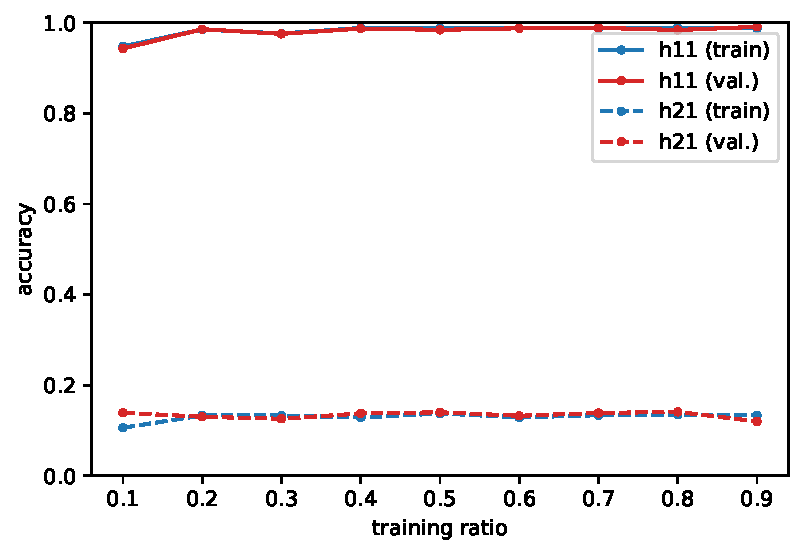
\includegraphics[width=0.45\linewidth]{img/linreg_learning_curve_num_cp_fav}
  \caption{%
    Learning curves for the linear regression (favourable dataset), including outliers and using a single model for both Hodge numbers.
    Input: \texttt{num\_cp}, $\alpha = 1$.
  }
  \label{fig:lc:lin-fav}
\end{figure}


\subsection{Support Vector Machines}
\label{sec:res:svr}

\svm are a family of algorithms which use a \emph{kernel trick} to map the space of input data vectors into a higher dimensional space where samples can be accurately separated and fitted to an appropriate curve (see~\Cref{sec:app:svr}).
In this analysis we show two such kernels, namely a linear kernel (also known as \emph{no kernel} since no transformations are involved) and a Gaussian kernel (known as \texttt{rbf} in \ml literature as in \emph{radial basis function}).


\subsubsection{Linear Kernel}

For this model we use the class \texttt{svm.LinearSVR} in \texttt{scikit-learn}.


\paragraph{Parameters}

In~\Cref{tab:hyp:linsvr} we show the choices of the hyperparameters used for the model.
As we prove in~\Cref{sec:app:svr}, parameters $C$ and $\epsilon$ are related to the penalty assigned to the samples lying outside the no-penalty boundary (the loss in this case is computed according to the $\ell_1$ or $\ell_2$ norm of the distance from the boundary as specified by the \texttt{loss} hyperparameter).
Other parameters are related to the use of the intercept to improve the prediction.
We rounded the predictions to the floor for the original dataset and to the next integer for the favourable dataset.

\begin{table}[tbp]
\centering
\resizebox{\linewidth}{!}{%
\begin{tabular}{@{}lccccccccc@{}}
\toprule
                                             &           & \multicolumn{2}{c}{\textbf{matrix}}                           & \multicolumn{2}{c}{\textbf{num\_cp}}                                            & \multicolumn{2}{c}{\textbf{eng. feat.}}                       & \multicolumn{2}{c}{\textbf{PCA}}                                       \\ \midrule
                                             &           & \textit{old}                  & \textit{fav.}                 & \textit{old}                           & \textit{fav.}                          & \textit{old}                  & \textit{fav.}                 & \textit{old}                           & \textit{fav.}                 \\ \midrule
\multirow{2}{*}{\texttt{C}}                  & \hodge{1}{1} & 0.13                          & 24                            & 0.001                                  & 0.0010                                 & 0.13                          & 0.001                         & 0.007                                  & 0.4                           \\
                                             & \hodge{2}{1} & 0.30                          & 100                           & 0.05                                  & 0.0016                                 & 0.5                          & 0.4                         & 1.5                                  & 0.4                           \\ \midrule
\multirow{2}{*}{$\epsilon$}                  & \hodge{1}{1} & 0.7                           & 0.3                           & 0.4                                    & 0.00                                   & 0.9                           & 0.0                           & 0.5                                    & 0.0                           \\
                                             & \hodge{2}{1} & 0.0                           & 0.0                           & 10                                   & 0.03                                   & 0.0                           & 0.0                           & 0.0                                    & 0.6                           \\ \midrule
\multirow{2}{*}{\texttt{fit\_intercept}}     & \hodge{1}{1} & True                          & False                         & True                                   & False                                  & True                          & False                         & False                                  & False                         \\
                                             & \hodge{2}{1} & True                          & False                         & True                                   & True                                   & True                          & True                          & True                                   & False                         \\ \midrule
\multirow{2}{*}{\texttt{intercept\_scaling}} & \hodge{1}{1} & 0.13                          & ---                           & 100                                    & ---                                    & 0.01                          & ---                           & ---                                    & ---                           \\
                                             & \hodge{2}{1} & 100                           & ---                           & 13                                     & 92                                     & 100                        & 0.01                          & 100                                    & ---                           \\ \midrule
\multirow{2}{*}{\texttt{loss}}               & \hodge{1}{1} & $\abs{\epsilon}$ & $\abs{\epsilon}$ & $\abs{\epsilon}$          & $\norm{\epsilon}^2$ & $\abs{\epsilon}$ & $\abs{\epsilon}$ & $\abs{\epsilon}$ & $\abs{\epsilon}$ \\
                                             & \hodge{2}{1} & $\abs{\epsilon}$ & $\abs{\epsilon}$ & $\norm{\epsilon}^2$ & $\abs{\epsilon}$          & $\abs{\epsilon}$ & $\abs{\epsilon}$ & $\abs{\epsilon}$          & $\abs{\epsilon}$ \\ \bottomrule
\end{tabular}%
}
\caption{%
  Hyperparameter choices of the linear support vector regression.
  The parameter \texttt{intercept\_scaling} is clearly only relevant when the intercept is used.
  The different losses used simply distinguish between the $\ell_1$ norm of the $\epsilon$-dependent boundary where no penalty is assigned and its $\ell_2$ norm.
}
\label{tab:hyp:linsvr}
\end{table}


\paragraph{Results}

In~\Cref{tab:res:linsvr}, we show the accuracy on the test set for the linear kernel.
As we can see, the performance of the algorithm strongly resembles a linear model in terms of the accuracy reached.
It is fascinating to notice that the contributions of the \pca do not improve the predictions using just the engineered features: it seems that the latter work better than using the configuration matrix or its principal components.

The residual plots in~\Cref{fig:res:linsvr} confirm what we already said about the linear models with regularisation: the model with only the number of projective spaces shows a tendency to heteroscedasticity which can be balanced by adding more engineered feature, also helping in having more precise predictions (translated into peaked univariate distributions).\footnotemark{}
\footnotetext{%
  Heteroscedasticity refers to the tendency to have a correlation between the predictions and the residuals: theoretically speaking, there should not be any, since we suppose the residuals to be independent on the model and normally sampled.
}
In all cases, we notice that the model slightly overestimates the real values (residuals are computed as the difference between the prediction and the real value) as the second, small peaks in the histograms for \hodge{1}{1} suggest: this may also explain why flooring the predictions produces the highest accuracy.
As in general for linear models, the influence of the number of samples used for training is marginal also in this case: we only noticed a decrease in accuracy when also including the \pca or directly the matrix.

\begin{table}[tbp]
\centering
\begin{tabular}{@{}cccccc@{}}
  \toprule
                          &           & \textbf{matrix} & \textbf{num\_cp} & \textbf{eng. feat.} & \textbf{PCA} \\ \midrule
    \multirow{2}{*}
    {\emph{original}}   & \hodge{1}{1} & \SI{61}{\percent}            & \SI{63}{\percent}             & \SI{65}{\percent}                & \SI{62}{\percent}         \\
                          & \hodge{2}{1} & \SI{11}{\percent}            & \SI{9}{\percent}              & \SI{21}{\percent}                & \SI{20}{\percent}         \\ \midrule
    \multirow{2}{*}
    {\emph{favourable}} & \hodge{1}{1} & \SI{96}{\percent}            & \SI{100}{\percent}            & \SI{100}{\percent}               & \SI{100}{\percent}        \\
                          & \hodge{2}{1} & \SI{14}{\percent}            & \SI{14}{\percent}             & \SI{19}{\percent}                & \SI{20}{\percent}         \\ \bottomrule
	\end{tabular}
	\caption{Accuracy of the linear \svm on the test split.}
	\label{tab:res:linsvr}
\end{table}


\begin{figure}[tbp]
  \centering
  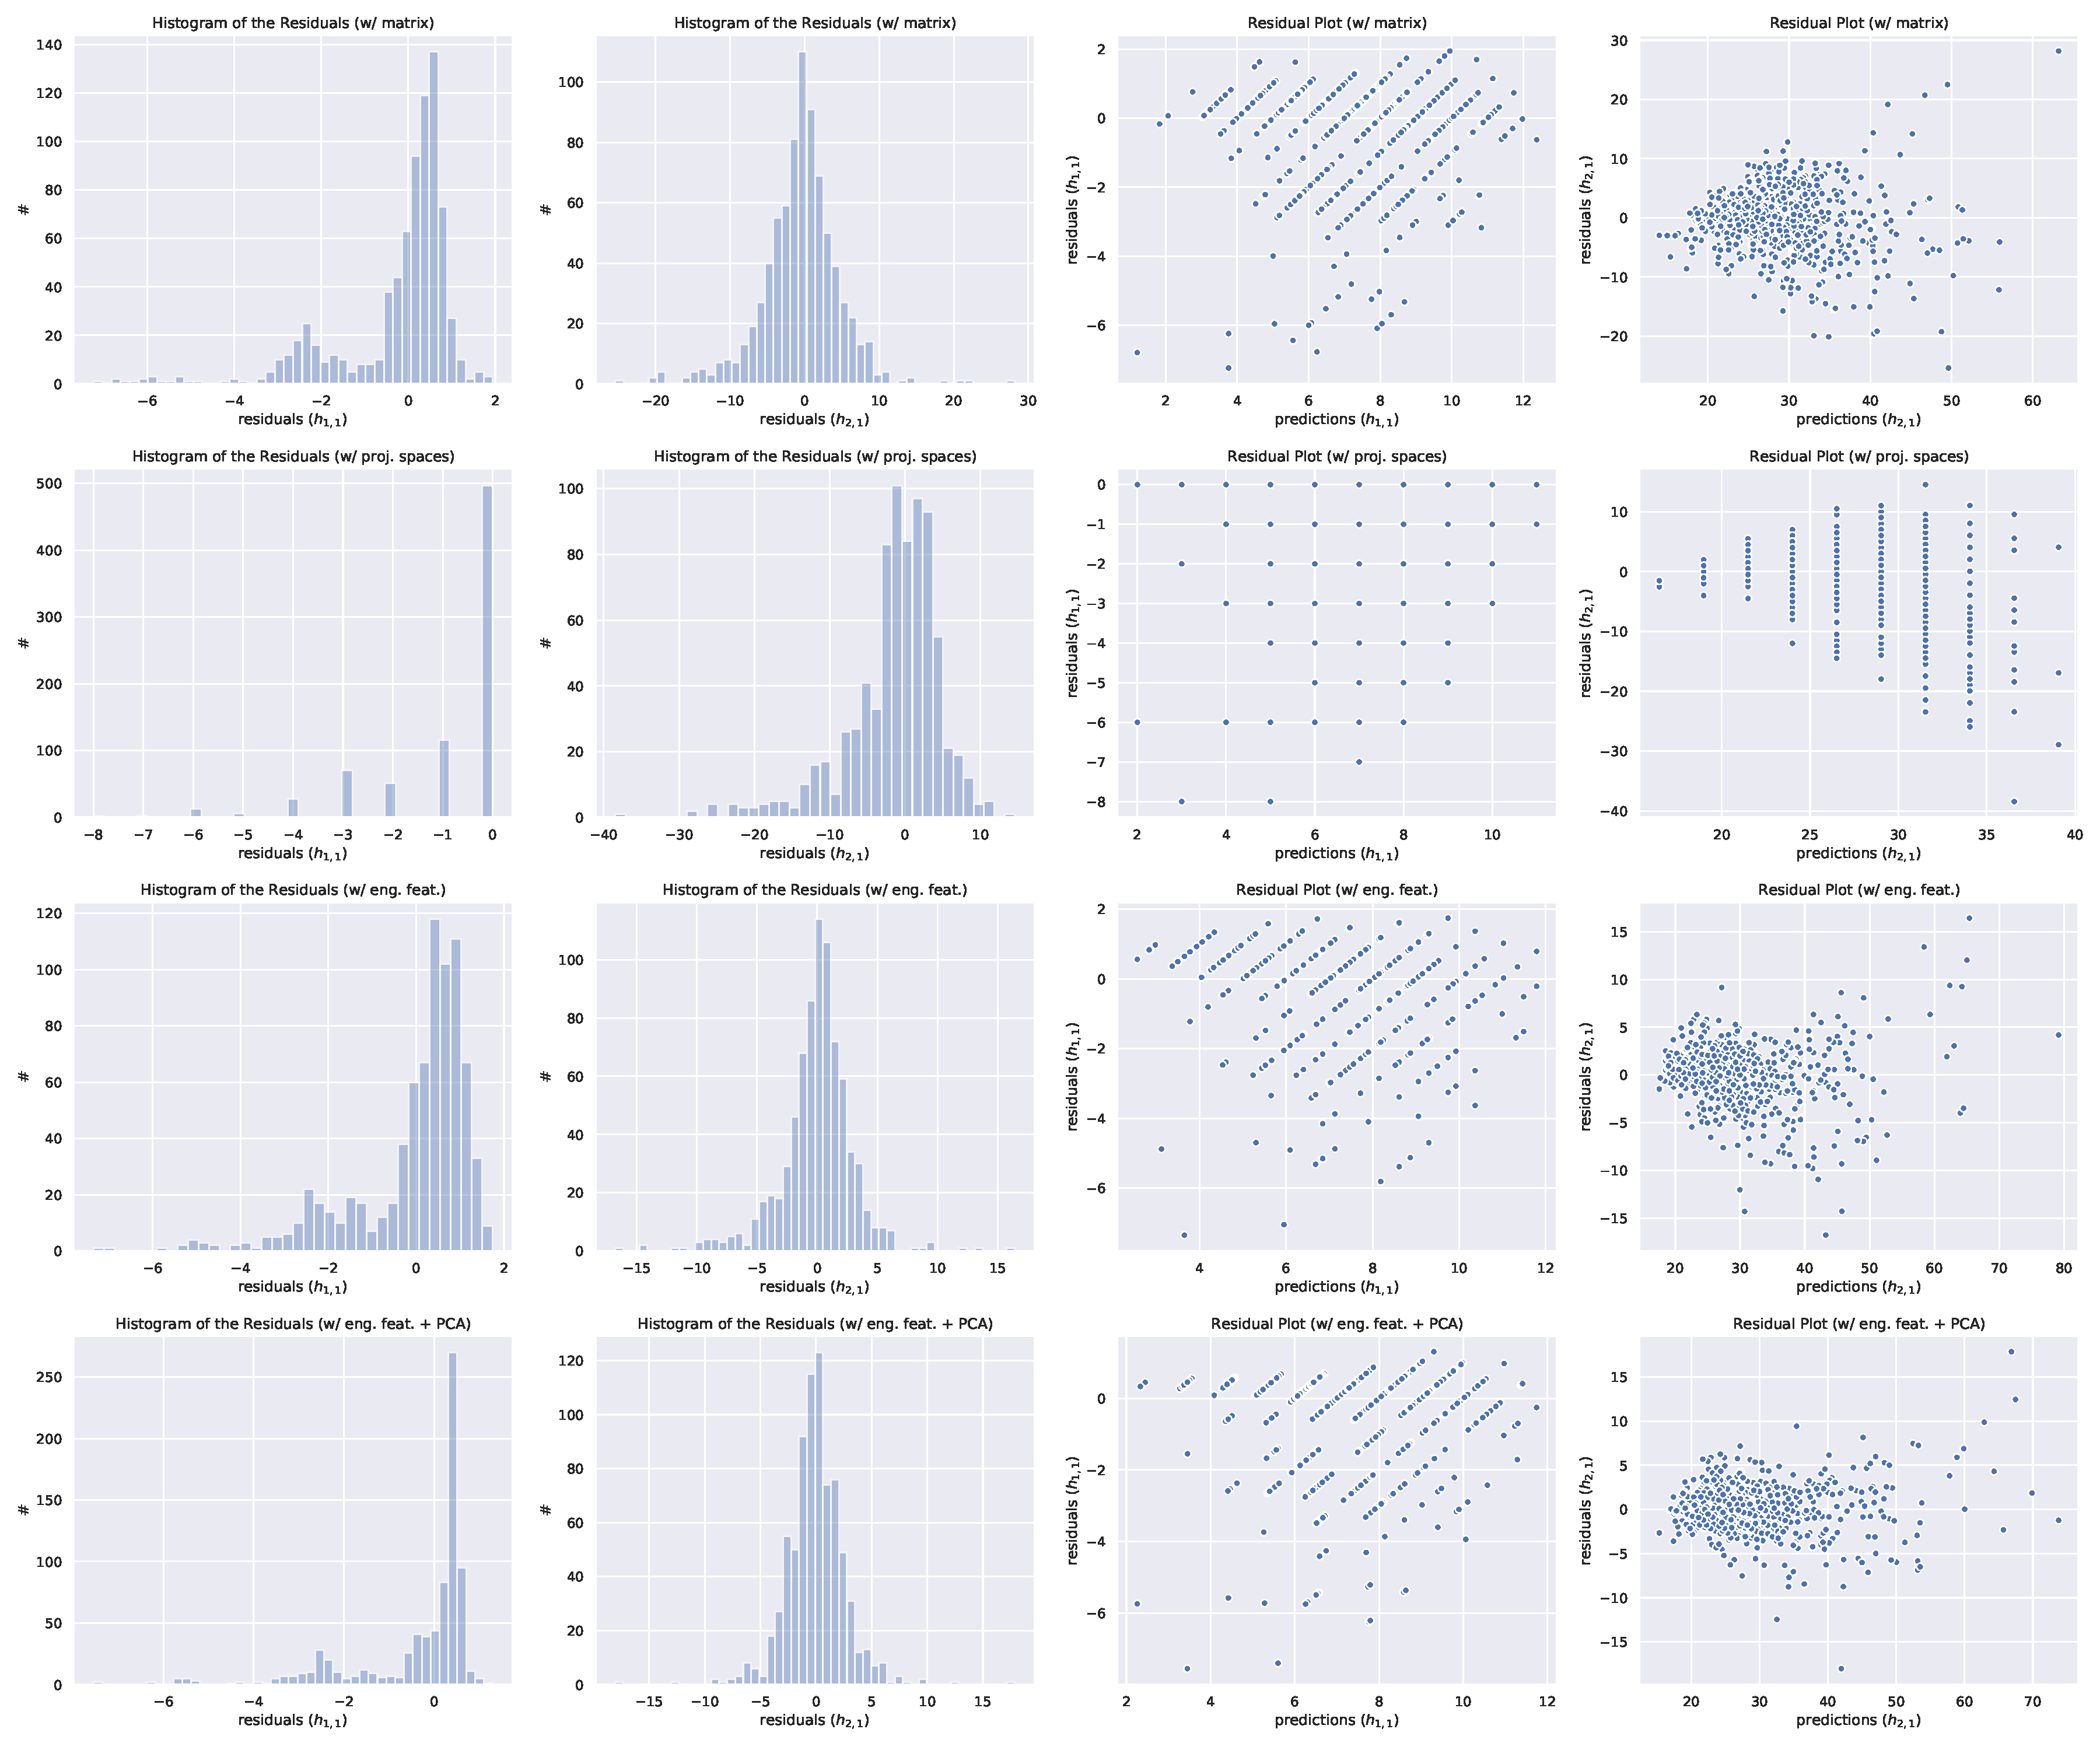
\includegraphics[width=0.9\linewidth]{img/lin_svr_orig}
  \caption{Plots of the residual errors for the \svm with linear kernel.}
  \label{fig:res:linsvr}
\end{figure}


\subsubsection{Gaussian Kernel}

We then consider \svm using a Gaussian function as kernel.
The choice of the function can heavily influence the outcome of the predictions since they map the samples into a much higher dimensional space and create highly non-linear combinations of the features before fitting the algorithm.
In general this can help in the presence of ``obscure'' features which badly correlate one another.
In our case we hope to leverage the already good correlations we found in the \eda with the kernel trick.
The implementation is done with the class \texttt{svm.SVR} from \texttt{scikit-learn}.


\paragraph{Parameters}

As we show in~\Cref{sec:app:svr}, this particular choice of kernel leads to profoundly different behaviour with respect to linear models: we will round the predictions to the next integer in both datasets since the loss function strongly penalises unaligned samples.
In~\Cref{tab:hyp:svrrbf} we show the choices of the hyperparameters for the models using the Gaussian kernel.
As usual the hyperparameter \texttt{C} is connected to the penalty assigned to the samples outside the soft margin boundary (see~\Cref{sec:app:svr}) delimited by the $\epsilon$.
Given the presence of a non linear kernel we have to introduce an additional hyperparameter $\gamma$ which controls the width of the Gaussian function used for the support vectors.

\begin{table}[tbp]
\centering
\begin{tabular}{@{}lccccccccc@{}}
\toprule
                            &           & \multicolumn{2}{c}{\textbf{matrix}} & \multicolumn{2}{c}{\textbf{num\_cp}} & \multicolumn{2}{c}{\textbf{eng. feat.}} & \multicolumn{2}{c}{\textbf{PCA}} \\ \midrule
                            &           & \textit{old}     & \textit{fav.}    & \textit{old}     & \textit{fav.}     & \textit{old}       & \textit{fav.}      & \textit{old}   & \textit{fav.}   \\ \midrule
\multirow{2}{*}{\texttt{C}} & \hodge{1}{1} & 14               & 1000             & 170              & 36                & 3                  & 40                 & 1.0            & 1000            \\
                            & \hodge{2}{1} & 40               & 1000             & 1.0              & 1.0               & 84                 & 62                 & 45             & 40              \\ \midrule
\multirow{2}{*}{$\epsilon$} & \hodge{1}{1} & 0.01             & 0.01             & 0.45             & 0.03              & 0.05               & 0.3                & 0.02           & 0.01            \\
                            & \hodge{2}{1} & 0.01             & 0.01             & 0.01             & 0.09              & 0.29               & 0.10               & 0.20           & 0.09            \\ \midrule
\multirow{2}{*}{$\gamma$}   & \hodge{1}{1} & 0.03             & 0.002            & 0.110            & 0.009             & 0.07               & 0.003              & 0.02           & 0.001           \\
                            & \hodge{2}{1} & 0.06             & 0.100            & 0.013            & 1000              & 0.016              & 0.005              & 0.013          & 0.006           \\ \bottomrule
\end{tabular}%
\caption{Hyperparameter choices of the \svm regression with Gaussian kernel.}
\label{tab:hyp:svrrbf}
\end{table}


\paragraph{Results}

In~\Cref{tab:res:svrrbf} we show the accuracy of the predictions on the test sets.
In the favourable dataset we can immediately appreciate the strong linear dependence of \hodge{1}{1} on the number of projective spaces: even though there are a few non favourable embeddings in the dataset, the kernel trick is able to map them in a better representation and improve the accuracy.
The predictions for the original dataset have also improved: they are the best results we found using shallow learning.
The predictions using only the configuration matrix matches~\cite{Bull:2018:MachineLearningCICY} but we can slightly improve the accuracy by using a combination of engineered features and \pca.
In~\Cref{fig:res:svrrbf} we show the residual plots and their histograms for the original dataset: residuals follow peaked distributions which, in this case, do not present a second smaller peak (thus we need to round to the next integer the predictions) and good variate distribution over the predictions.

The Gaussian kernel is also more influenced by the size of the training set.
Using \SI{50}{\percent} of the samples as training set we witnessed a drop in accuracy of \SI{3}{\percent} while using engineered features and the \pca, and around \SI{1}{\percent} to \SI{2}{\percent} in all other cases.
The learning curves (presented in~\Cref{fig:lc:svrrbf}) show that the accuracy improves by using more data.
Interestingly, it shows that using all engineered features leads to an overfit on the training data since both Hodge numbers reach almost \SI{100}{\percent}, while this is not the case for \hodge{2}{1}.
For comparison, we also display in \Cref{fig:lc:svrrbf-fav} the learning curve for the favourable dataset: this shows that predicting \hodge{1}{1} accurately works out-of-the-box.

\begin{table}[tbp]
\centering
\begin{tabular}{@{}cccccc@{}}
  \toprule
                          &           & \textbf{matrix} & \textbf{num\_cp} & \textbf{eng. feat.} & \textbf{PCA} \\ \midrule
    \multirow{2}{*}
    {\emph{original}}   & \hodge{1}{1} & \SI{70}{\percent}            & \SI{63}{\percent}             & \SI{66}{\percent}                & \SI{72}{\percent}         \\
                          & \hodge{2}{1} & \SI{22}{\percent}            & \SI{10}{\percent}             & \SI{36}{\percent}                & \SI{34}{\percent}         \\ \midrule
    \multirow{2}{*}
    {\emph{favourable}} & \hodge{1}{1} & \SI{99}{\percent}            & \SI{100}{\percent}            & \SI{100}{\percent}               & \SI{100}{\percent}        \\
                          & \hodge{2}{1} & \SI{22}{\percent}            & \SI{17}{\percent}             & \SI{32}{\percent}                & \SI{33}{\percent}         \\ \bottomrule
\end{tabular}
\caption{Accuracy of the Gaussian \svm on the test split.}
\label{tab:res:svrrbf}
\end{table}

\begin{figure}[tbp]
  \centering
  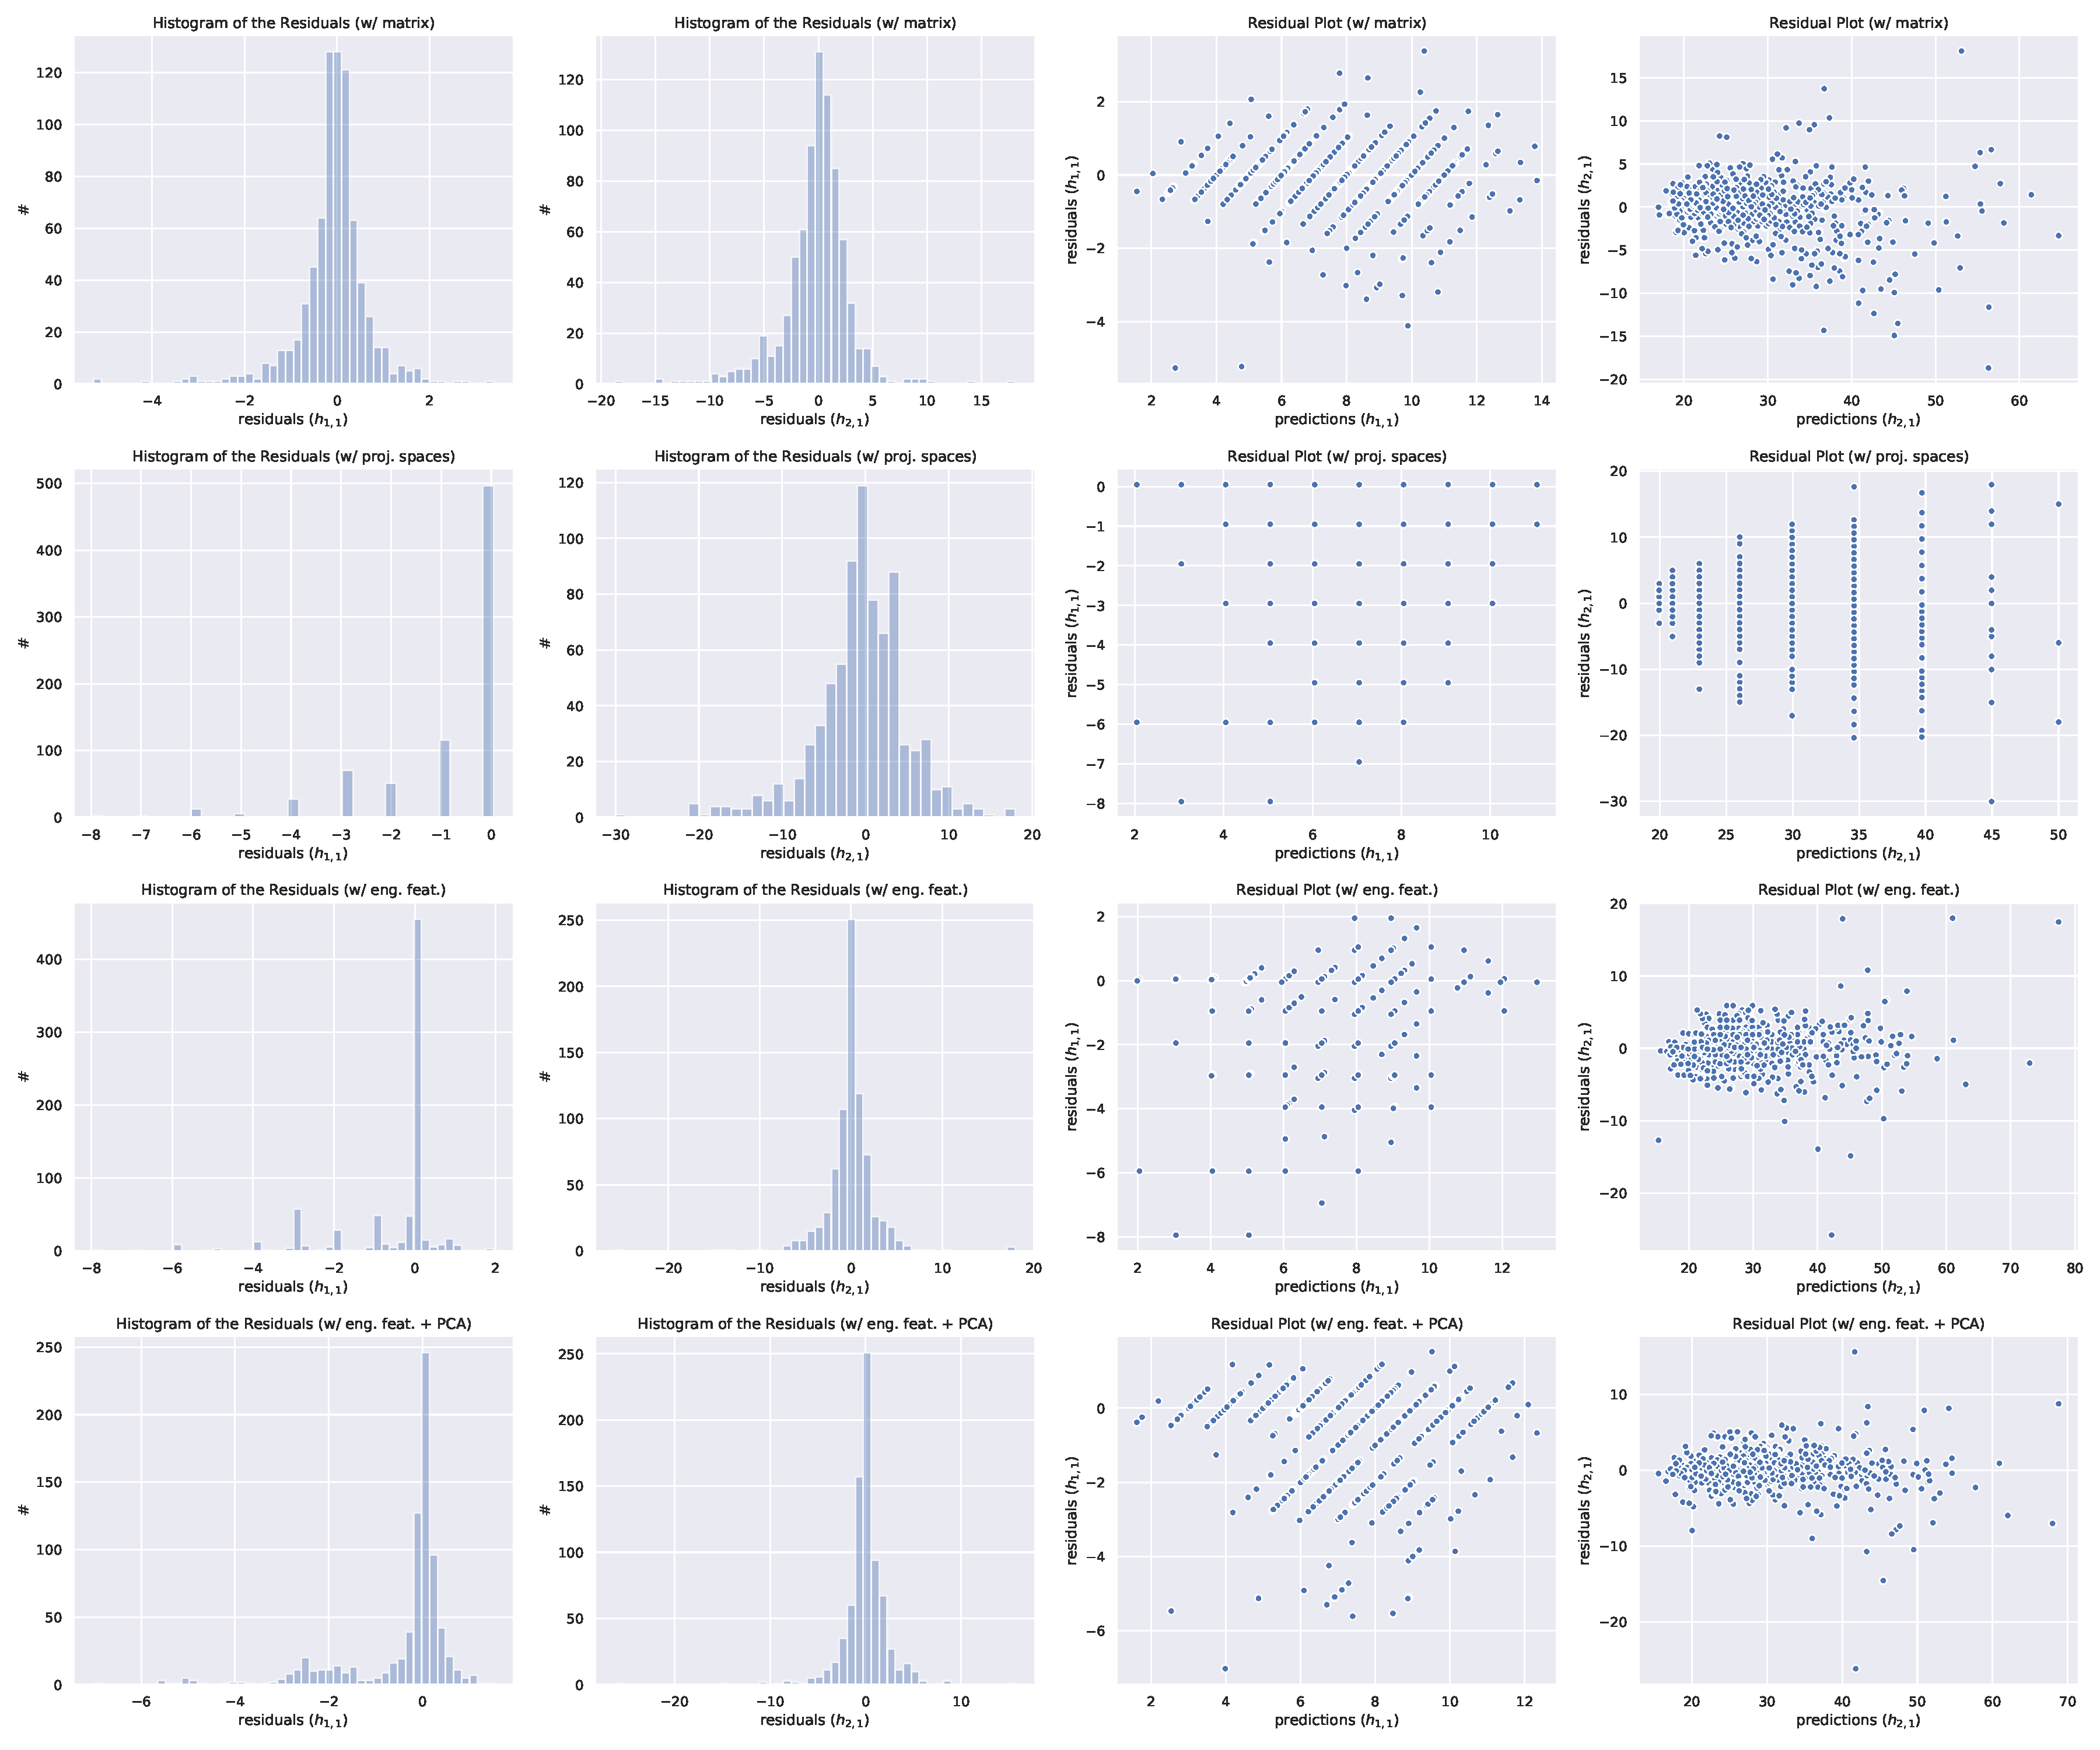
\includegraphics[width=\linewidth]{img/svr_rbf_orig}
  \caption{Plots of the residual errors for the \svm with Gaussian kernel.}
  \label{fig:res:svrrbf}
\end{figure}


\begin{figure}[htp]
  \centering
  \begin{subfigure}[c]{0.45\linewidth}
    \centering
    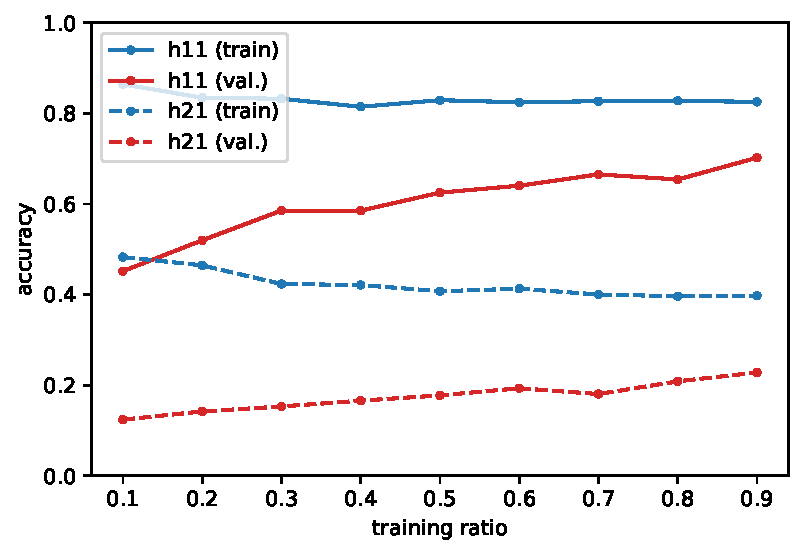
\includegraphics[width=\linewidth]{img/svm_learning_curve_matrix_outliers}
    \caption{input: \texttt{matrix}, $C = 15, \gamma = 0.03, \epsilon = 0.1$}
  \end{subfigure}
  \hfill
  \begin{subfigure}[c]{0.45\linewidth}
    \centering
    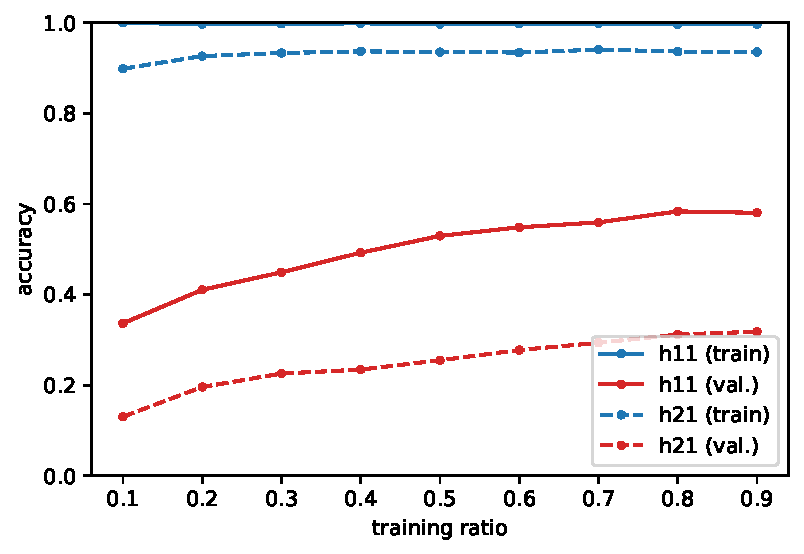
\includegraphics[width=\linewidth]{img/svm_learning_curve_all_outliers}
    \caption{input: all, $C = 10, \gamma = 0.03, \epsilon = 0.1$}
  \end{subfigure}
  \caption{%
    Learning curves for the \svm with Gaussian kernel (original dataset), using a single model for both Hodge numbers.
  }
  \label{fig:lc:svrrbf}
\end{figure}

\begin{figure}[tbp]
  \centering
  \begin{subfigure}[c]{0.45\linewidth}
    \centering
    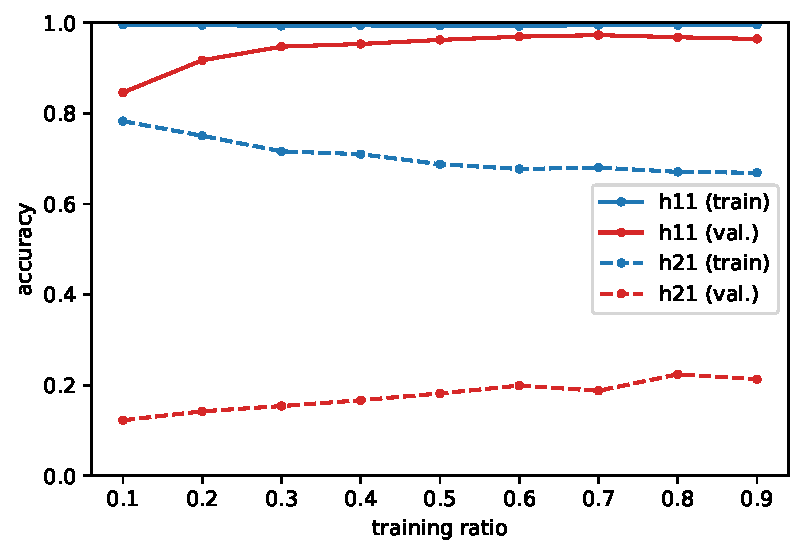
\includegraphics[width=\linewidth]{img/svm_learning_curve_matrix_fav}
    \caption{input: \texttt{matrix}, $C = 20, \gamma = \mathtt{scale}, \epsilon = 0.1$}
  \end{subfigure}
  \hfill
  \begin{subfigure}[c]{0.45\linewidth}
    \centering
    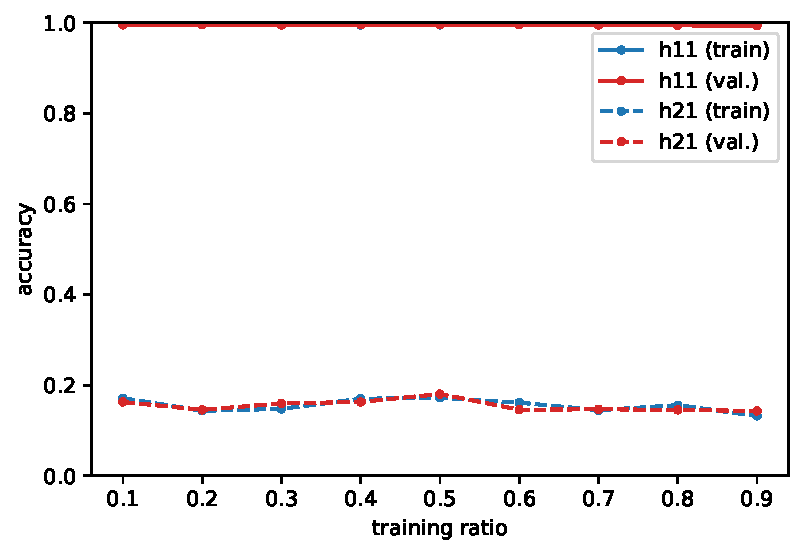
\includegraphics[width=\linewidth]{img/svm_learning_curve_num_cp_fav}
    \caption{input: all, $C = 20, \gamma = \mathtt{scale}, \epsilon = 0.1$}
  \end{subfigure}
  \caption{%
    Learning curves for the \svm with Gaussian kernel (favourable dataset), using a single model for both Hodge numbers.
  }
  \label{fig:lc:svrrbf-fav}
\end{figure}


\subsection{Decision Trees}
\label{sec:ml:trees}

We now consider two algorithms based on decision trees: random forests and gradient boosted trees.
Decision trees are powerful algorithms which implement a simple decision rule (in the style of an \emph{if\dots then\dots else\dots} statement) to classify or assign a value to the predictions.
However they have a tendency to adapt too well to the training set and to not be robust enough against small changes in the training data.
We consider a generalisation of this algorithm used for \emph{ensemble learning}: this is a technique in \ml which uses multiple estimators (they can be the same or different) to improve the performances.
We will present the results of \emph{random forests} of trees which increase the bias compared to a single decision tree, and \emph{gradient boosted} decision trees, which can use smaller trees to decrease the variance and learn better representations of the input data by iterating their decision functions and use information on the previous runs to improve (see~\Cref{sec:app:trees} for a more in-depth description).


\subsubsection{Random Forests}

The random forest algorithm is implemented with Scikit's \texttt{ensemble.RandomForestRegressor}.


\paragraph{Parameters}

Hyperparameter tuning for decision trees can in general be quite challenging.
From the general theory on random forests (see~\Cref{sec:app:trees} for salient features) we can try and look for particular shapes of the trees: this ensemble learning technique usually prefers a small number of fully grown trees.
We performed only 25 iterations of the optimisation process due to the very long time taken to train all the decision trees.

In~\Cref{tab:hyp:rndfor} we show the hyperparameters used for the predictions.
As we can see from \texttt{n\_estimator}, random forests are usually built with a small number of fully grown (specified by \texttt{max\_depth} and \texttt{max\_leaf\_nodes}) trees (not always the case, though).
In order to avoid overfit we also tried to increase the number of samples necessary to split a branch or create a leaf node using \texttt{min\_samples\_leaf} and \texttt{min\_samples\_split} (introducing also a weight on the samples in the leaf nodes specified by \texttt{min\_weight\_fraction\_leaf} to balance the tree).
Finally the \texttt{criterion} chosen by the optimisation reflects the choice of the trees to measure the impurity of the predictions using either the mean squared error or the mean absolute error of the predictions (see \Cref{sec:app:trees}).

\begin{table}[tbp]
\centering
\resizebox{\linewidth}{!}{%
\begin{tabular}{@{}lccccccccc@{}}
\toprule
                                                      &           & \multicolumn{2}{c}{\textbf{matrix}}  & \multicolumn{2}{c}{\textbf{num\_cp}}        & \multicolumn{2}{c}{\textbf{eng. feat.}} & \multicolumn{2}{c}{\textbf{PCA}} \\ \midrule
                                                      &           & \textit{old}         & \textit{fav.} & \textit{old}         & \textit{fav.}        & \textit{old}   & \textit{fav.}          & \textit{old}   & \textit{fav.}   \\ \midrule
\multirow{2}{*}{\texttt{criterion}}                            & \hodge{1}{1} & \mse         & \mse  & \mae         & \mae         & \mae   & \mse           & \mae   & \mae    \\
                                                      & \hodge{2}{1} & \mae         & \mae  & \mae         & \mae         & \mae   & \mae           & \mae   & \mae    \\ \midrule
\multirow{2}{*}{\texttt{max\_depth}}                  & \hodge{1}{1} & 100                  & 100           & 100                  & 30                   & 90             & 30                     & 30             & 60              \\
                                                      & \hodge{2}{1} & 90                   & 100           & 90                   & 75                   & 100            & 100                    & 100            & 60              \\ \midrule
\multirow{2}{*}{\texttt{max\_leaf\_nodes}}            & \hodge{1}{1} & 100                  & 80            & 90                   & 20                   & 20             & 35                     & 90             & 90              \\
                                                      & \hodge{2}{1} & 90                   & 100           & 100                  & 75                   & 100            & 60                     & 100            & 100             \\ \midrule
\multirow{2}{*}{\texttt{min\_samples\_leaf}}          & \hodge{1}{1} & 1                    & 1             & 1                    & 15                   & 1              & 15                     & 1              & 1               \\
                                                      & \hodge{2}{1} & 3                    & 1             & 4                    & 70                   & 1              & 70                     & 30             & 1               \\ \midrule
\multirow{2}{*}{\texttt{min\_samples\_split}}         & \hodge{1}{1} & 2                    & 30            & 20                   & 35                   & 10             & 10                     & 100            & 100             \\
                                                      & \hodge{2}{1} & 30                   & 2             & 50                   & 45                   & 2              & 100                    & 2              & 100             \\ \midrule
\multirow{2}{*}{\texttt{min\_weight\_fraction\_leaf}} & \hodge{1}{1} & 0.0                  & 0.0           & 0.0                  & $1.7 \times 10^{-3}$ & 0.0            & 0.009   & 0.0            & 0.0             \\
                                                      & \hodge{2}{1} & $3.0 \times 10^{-4}$ & 0.0           & $1.0 \times 10^{-4}$ & 0.13                 & 0.0            & 0.0                    & 0.0            & 0.0             \\ \midrule
\multirow{2}{*}{\texttt{n\_estimators}}               & \hodge{1}{1} & 10                   & 100           & 45                   & 120                  & 155            & 300                    & 10             & 300             \\
                                                      & \hodge{2}{1} & 190                  & 10            & 160                  & 300                  & 10             & 10                     & 10             & 300             \\ \bottomrule
\end{tabular}%
}
\caption{Hyperparameter choices of the random forest regression.}
\label{tab:hyp:rndfor}
\end{table}


\paragraph{Results}

In~\Cref{tab:res:rndfor} we summarise the accuracy reached using random forests of decision trees as estimators.
As we already expected, the contribution of the number of projective spaces helps the algorithm to generate better predictions.
In general, it seems that the engineered features alone can already provide a good basis for predictions.
In the case of \hodge{2}{1} the introduction of the principal components of the configuration matrix also increases the prediction capabilities.
As in most other cases we used the floor function for the predictions on the original dataset and the rounding to next integer for the favourable one.

As usual in~\Cref{fig:res:rndfor} we show the histograms of the distribution of the residual errors and the scatter plots of the residuals.
While the distributions of the errors are slightly wider than the \svm algorithms, the scatter plots of the residual show a strong heteroscedasticity in the case of the fit using the number of projective spaces: though quite accurate, the model is strongly incomplete.
The inclusion of the other engineered features definitely helps and also leads to better predictions.
Learning curves are displayed in~\Cref{fig:lc:rndfor}.

\begin{table}[tbp]
\centering
\begin{tabular}{@{}cccccc@{}}
  \toprule
                          &           & \textbf{matrix} & \textbf{num\_cp} & \textbf{eng. feat.} & \textbf{PCA} \\ \midrule
    \multirow{2}{*}
    {\emph{original}}   & \hodge{1}{1} & \SI{55}{\percent}            & \SI{63}{\percent}             & \SI{66}{\percent}                & \SI{64}{\percent}         \\
                          & \hodge{2}{1} & \SI{12}{\percent}            & \SI{9}{\percent}              & \SI{17}{\percent}                & \SI{18}{\percent}         \\ \midrule
    \multirow{2}{*}
    {\emph{favourable}} & \hodge{1}{1} & \SI{89}{\percent}            & \SI{99}{\percent}             & \SI{98}{\percent}                & \SI{98}{\percent}         \\
                          & \hodge{2}{1} & \SI{14}{\percent}            & \SI{17}{\percent}             & \SI{22}{\percent}                & \SI{27}{\percent}         \\ \bottomrule
\end{tabular}
\caption{Accuracy of the random forests on the test split.}
\label{tab:res:rndfor}
\end{table}

\begin{figure}[tbp]
  \centering
  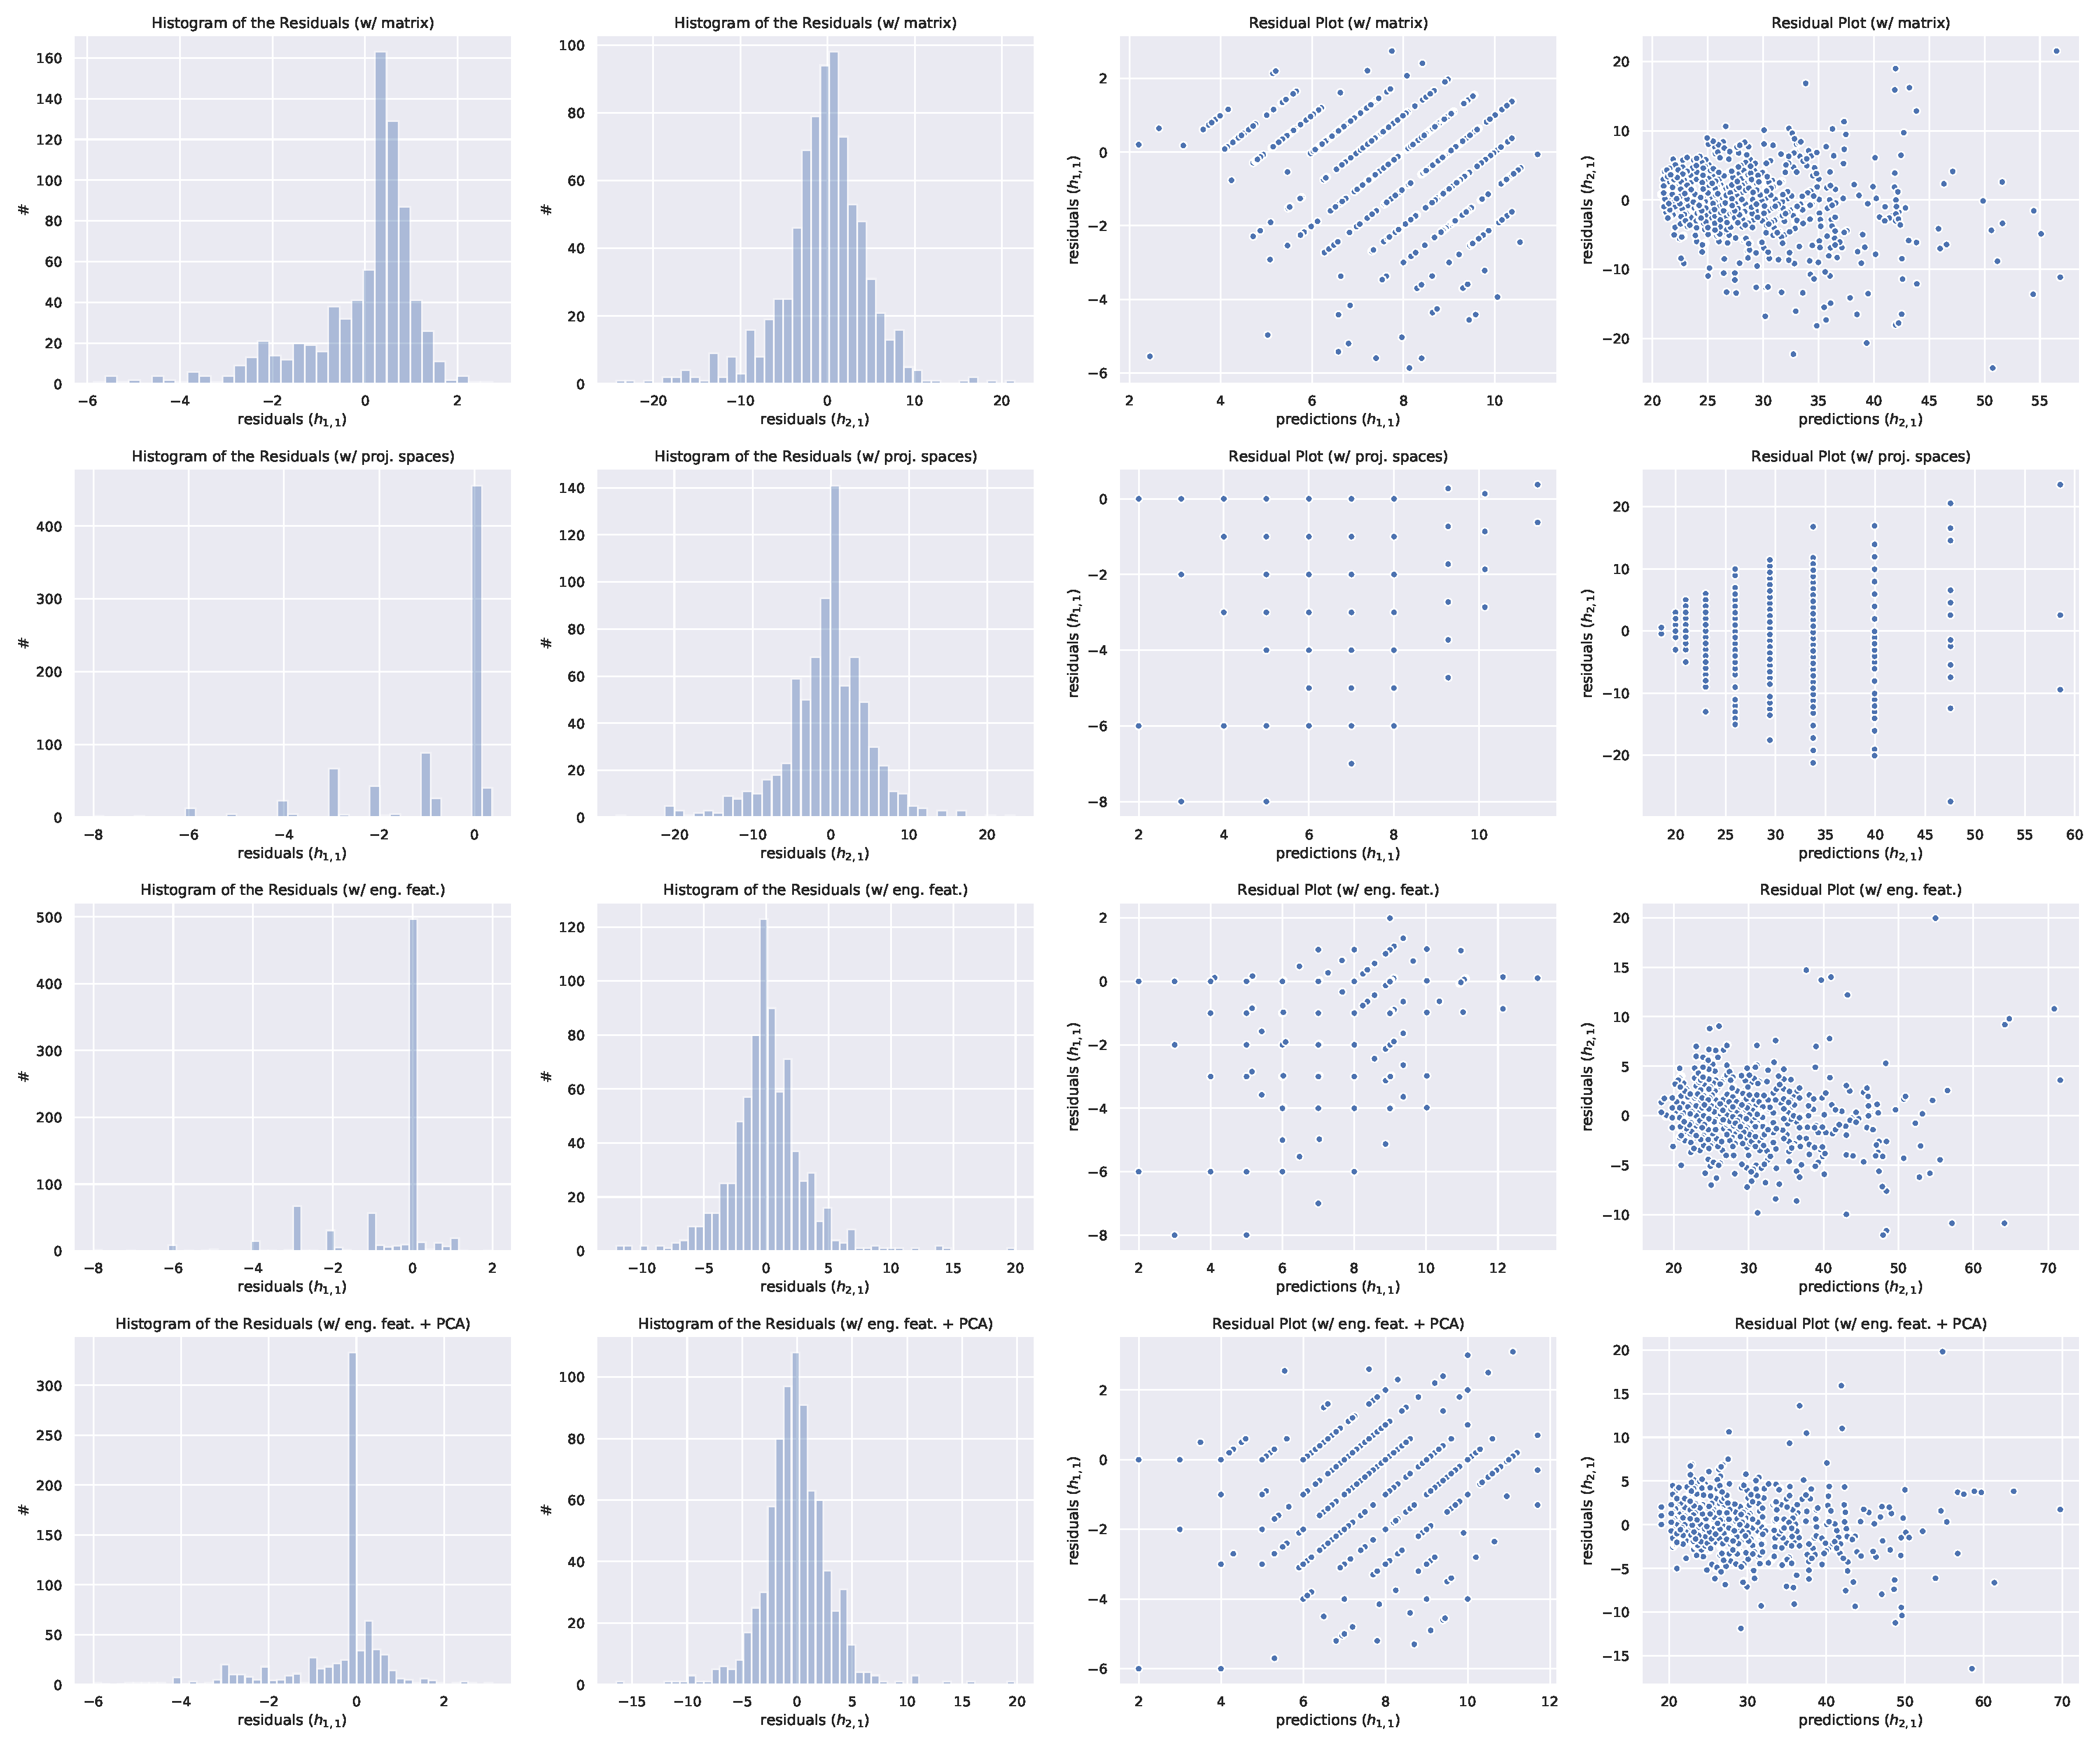
\includegraphics[width=0.9\linewidth]{img/rnd_for_orig}
  \caption{Plots of the residual errors for the random forests.}
  \label{fig:res:rndfor}
\end{figure}

\begin{figure}[tbp]
  \centering
  \begin{subfigure}[c]{0.45\linewidth}
          \centering
          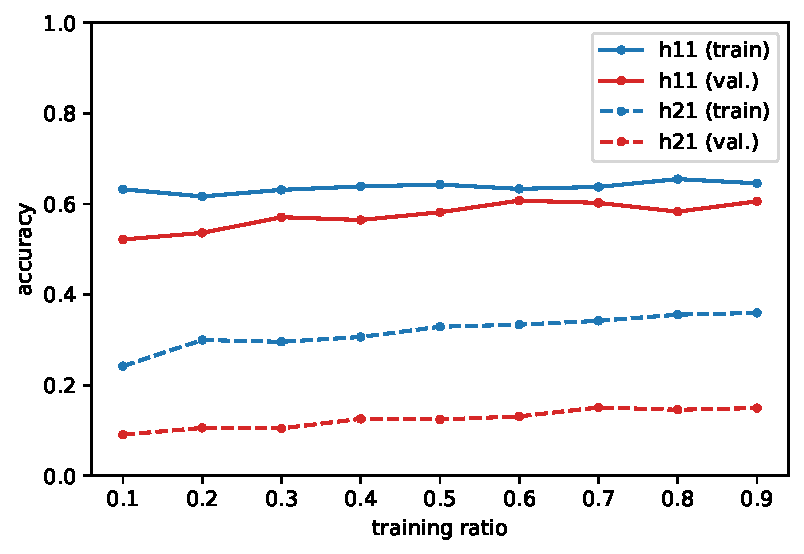
\includegraphics[width=\linewidth]{img/forest_learning_curve_matrix_outliers}
          \caption{input: \lstinline!matrix!, default parameters}
  \end{subfigure}
  \hfill
  \begin{subfigure}[c]{0.45\linewidth}
          \centering
          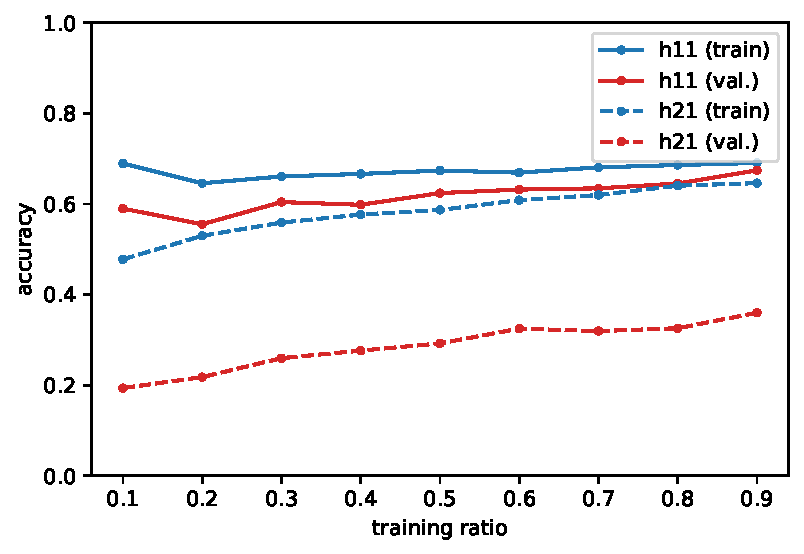
\includegraphics[width=\linewidth]{img/forest_learning_curve_all_outliers}
          \caption{input: all, default parameters}
  \end{subfigure}
  \caption{%
    Learning curves for the random forest (original dataset) including outliers and using a single model for both Hodge numbers.
  }
  \label{fig:lc:rndfor}
\end{figure}


\subsubsection{Gradient Boosted Trees}

We used the class \texttt{ensemble.GradientBoostingRegressor} in \texttt{scikit-learn} to implement the gradient boosted trees.


\paragraph{Parameters}

Hyperparameter optimisation has been performed using 25 iterations of the Bayes search algorithm since by comparison the gradient boosting algorithms took the longest learning time.
We show the chosen hyperparameters in~\Cref{tab:hyp:grdbst}.

With respect to the random forests, for the gradient boosting we also need to introduce the \texttt{learning\_rate} (or \emph{shrinking parameter}) which controls the gradient descent of the optimisation which is driven by the choice of the \texttt{loss} parameters (\texttt{ls} is the ordinary least squares loss, \texttt{lad} is the least absolute deviation and \texttt{huber} is a combination of the previous two losses weighted by the hyperparameter $\alpha$).
We also introduce the \texttt{subsample} hyperparameter which chooses a fraction of the samples to be fed into the algorithm at each iteration.
This procedure has both a regularisation effect on the trees, which should not adapt too much to the training set, and speeds up the training (at least by a very small amount).

\begin{table}[tbp]
\centering
\resizebox{\linewidth}{!}{%
\begin{tabular}{@{}lccccccccc@{}}
\toprule
                                                      &           & \multicolumn{2}{c}{\textbf{matrix}} & \multicolumn{2}{c}{\textbf{num\_cp}}   & \multicolumn{2}{c}{\textbf{eng. feat.}}         & \multicolumn{2}{c}{\textbf{PCA}} \\ \midrule
                                                      &           & \textit{old}     & \textit{fav.}    & \textit{old}           & \textit{fav.} & \textit{old}           & \textit{fav.}          & \textit{old}   & \textit{fav.}   \\ \midrule
\multirow{2}{*}{$\alpha$}                             & \hodge{1}{1} & 0.4              & ---              & ---                    & ---           & ---                    & ---                    & ---            & ---             \\
                                                      & \hodge{2}{1} & ---              & 0.11             & ---                    & ---           & 0.99                   & ---                    & ---            & ---             \\ \midrule
\multirow{2}{*}{\texttt{criterion}}                   & \hodge{1}{1} & \mae     & \mae     & \texttt{friedman\_mse} & \mae  & \texttt{friedman\_mse} & \texttt{friedman\_mse} & \mae   & \mae    \\
                                                      & \hodge{2}{1} & \mae     & \mae     & \texttt{friedman\_mse} & \mae  & \mae           & \mae           & \mae   & \mae    \\ \midrule
\multirow{2}{*}{\texttt{learning\_rate}}              & \hodge{1}{1} & 0.3              & 0.04             & 0.6                    & 0.03          & 0.15                   & 0.5                    & 0.04           & 0.03            \\
                                                      & \hodge{2}{1} & 0.6              & 0.5              & 0.3                    & 0.5           & 0.04                   & 0.02                   & 0.03           & 0.07            \\ \midrule
\multirow{2}{*}{\texttt{loss}}                        & \hodge{1}{1} & huber            & ls               & lad                    & ls            & ls                     & lad                    & ls             & ls              \\
                                                      & \hodge{2}{1} & ls               & huber            & ls                     & ls            & huber                  & ls                     & ls             & lad             \\ \midrule
\multirow{2}{*}{\texttt{max\_depth}}                  & \hodge{1}{1} & 100              & 100              & 15                     & 60            & 2                      & 100                    & 55             & 2               \\
                                                      & \hodge{2}{1} & 85               & 100              & 100                    & 30            & 35                     & 60                     & 15             & 2               \\ \midrule
\multirow{2}{*}{\texttt{min\_samples\_split}}         & \hodge{1}{1} & 2                & 30               & 20                     & 35            & 10                     & 10                     & 100            & 100             \\
                                                      & \hodge{2}{1} & 30               & 2                & 50                     & 45            & 2                      & 100                    & 2              & 100             \\ \midrule
\multirow{2}{*}{\texttt{min\_weight\_fraction\_leaf}} & \hodge{1}{1} & 0.03             & 0.0              & 0.0                    & 0.2           & 0.2                    & 0.0                    & 0.06           & 0.0             \\
                                                      & \hodge{2}{1} & 0.0              & 0.0              & 0.16                   & 0.004         & 0.0                    & 0.0                    & 0.0            & 0.0             \\ \midrule
\multirow{2}{*}{\texttt{n\_estimators}}               & \hodge{1}{1} & 90               & 240              & 120                    & 220           & 100                    & 130                    & 180            & 290             \\
                                                      & \hodge{2}{1} & 100              & 300              & 10                     & 20            & 200                    & 300                    & 300            & 300             \\ \midrule
\multirow{2}{*}{\texttt{subsample}}                   & \hodge{1}{1} & 0.8              & 0.8              & 0.9                    & 0.6           & 0.1                    & 0.1                    & 1.0            & 0.9             \\
                                                      & \hodge{2}{1} & 0.7              & 1.0              & 0.1                    & 0.9           & 0.1                    & 0.9                    & 0.1            & 0.2             \\ \bottomrule
\end{tabular}%
}
\caption{Hyperparameter choices of the gradient boosted decision trees.}
\label{tab:hyp:grdbst}
\end{table}


\paragraph{Results}

We show the results of gradient boosting in~\Cref{tab:res:grdbst}.
As usual the linear dependence of \hodge{1}{1} on the number of projective spaces is evident and in this case also produces the best accuracy result (using the floor function for the original dataset and rounding to the next integer for the favourable dataset) for \hodge{1}{1}.
\hodge{2}{1} is once again strongly helped by the presence of the redundant features.
In~\Cref{fig:res:grdbst} we finally show the histograms and the scatter plots of the residual errors for the original dataset showing that also in this case the choice of the floor function can be justified and that the addition of the engineered features certainly improves the overall variance of the residuals.

\begin{table}[tbp]
\centering
\begin{tabular}{@{}cccccc@{}}
  \toprule
                          &           & \textbf{matrix} & \textbf{num\_cp} & \textbf{eng. feat.} & \textbf{PCA} \\ \midrule
    \multirow{2}{*}
    {\emph{original}}   & \hodge{1}{1} & \SI{50}{\percent}            & \SI{63}{\percent}             & \SI{61}{\percent}                & \SI{58}{\percent}         \\
                          & \hodge{2}{1} & \SI{14}{\percent}            & \SI{9}{\percent}              & \SI{23}{\percent}                & \SI{21}{\percent}         \\ \midrule
    \multirow{2}{*}
    {\emph{favourable}} & \hodge{1}{1} & \SI{97}{\percent}            & \SI{100}{\percent}            & \SI{99}{\percent}                & \SI{99}{\percent}         \\
                          & \hodge{2}{1} & \SI{17}{\percent}            & \SI{16}{\percent}             & \SI{35}{\percent}                & \SI{22}{\percent}         \\ \bottomrule
\end{tabular}
\caption{Accuracy of the gradient boosting on the test split.}
\label{tab:res:grdbst}
\end{table}

\begin{figure}[tbp]
  \centering
  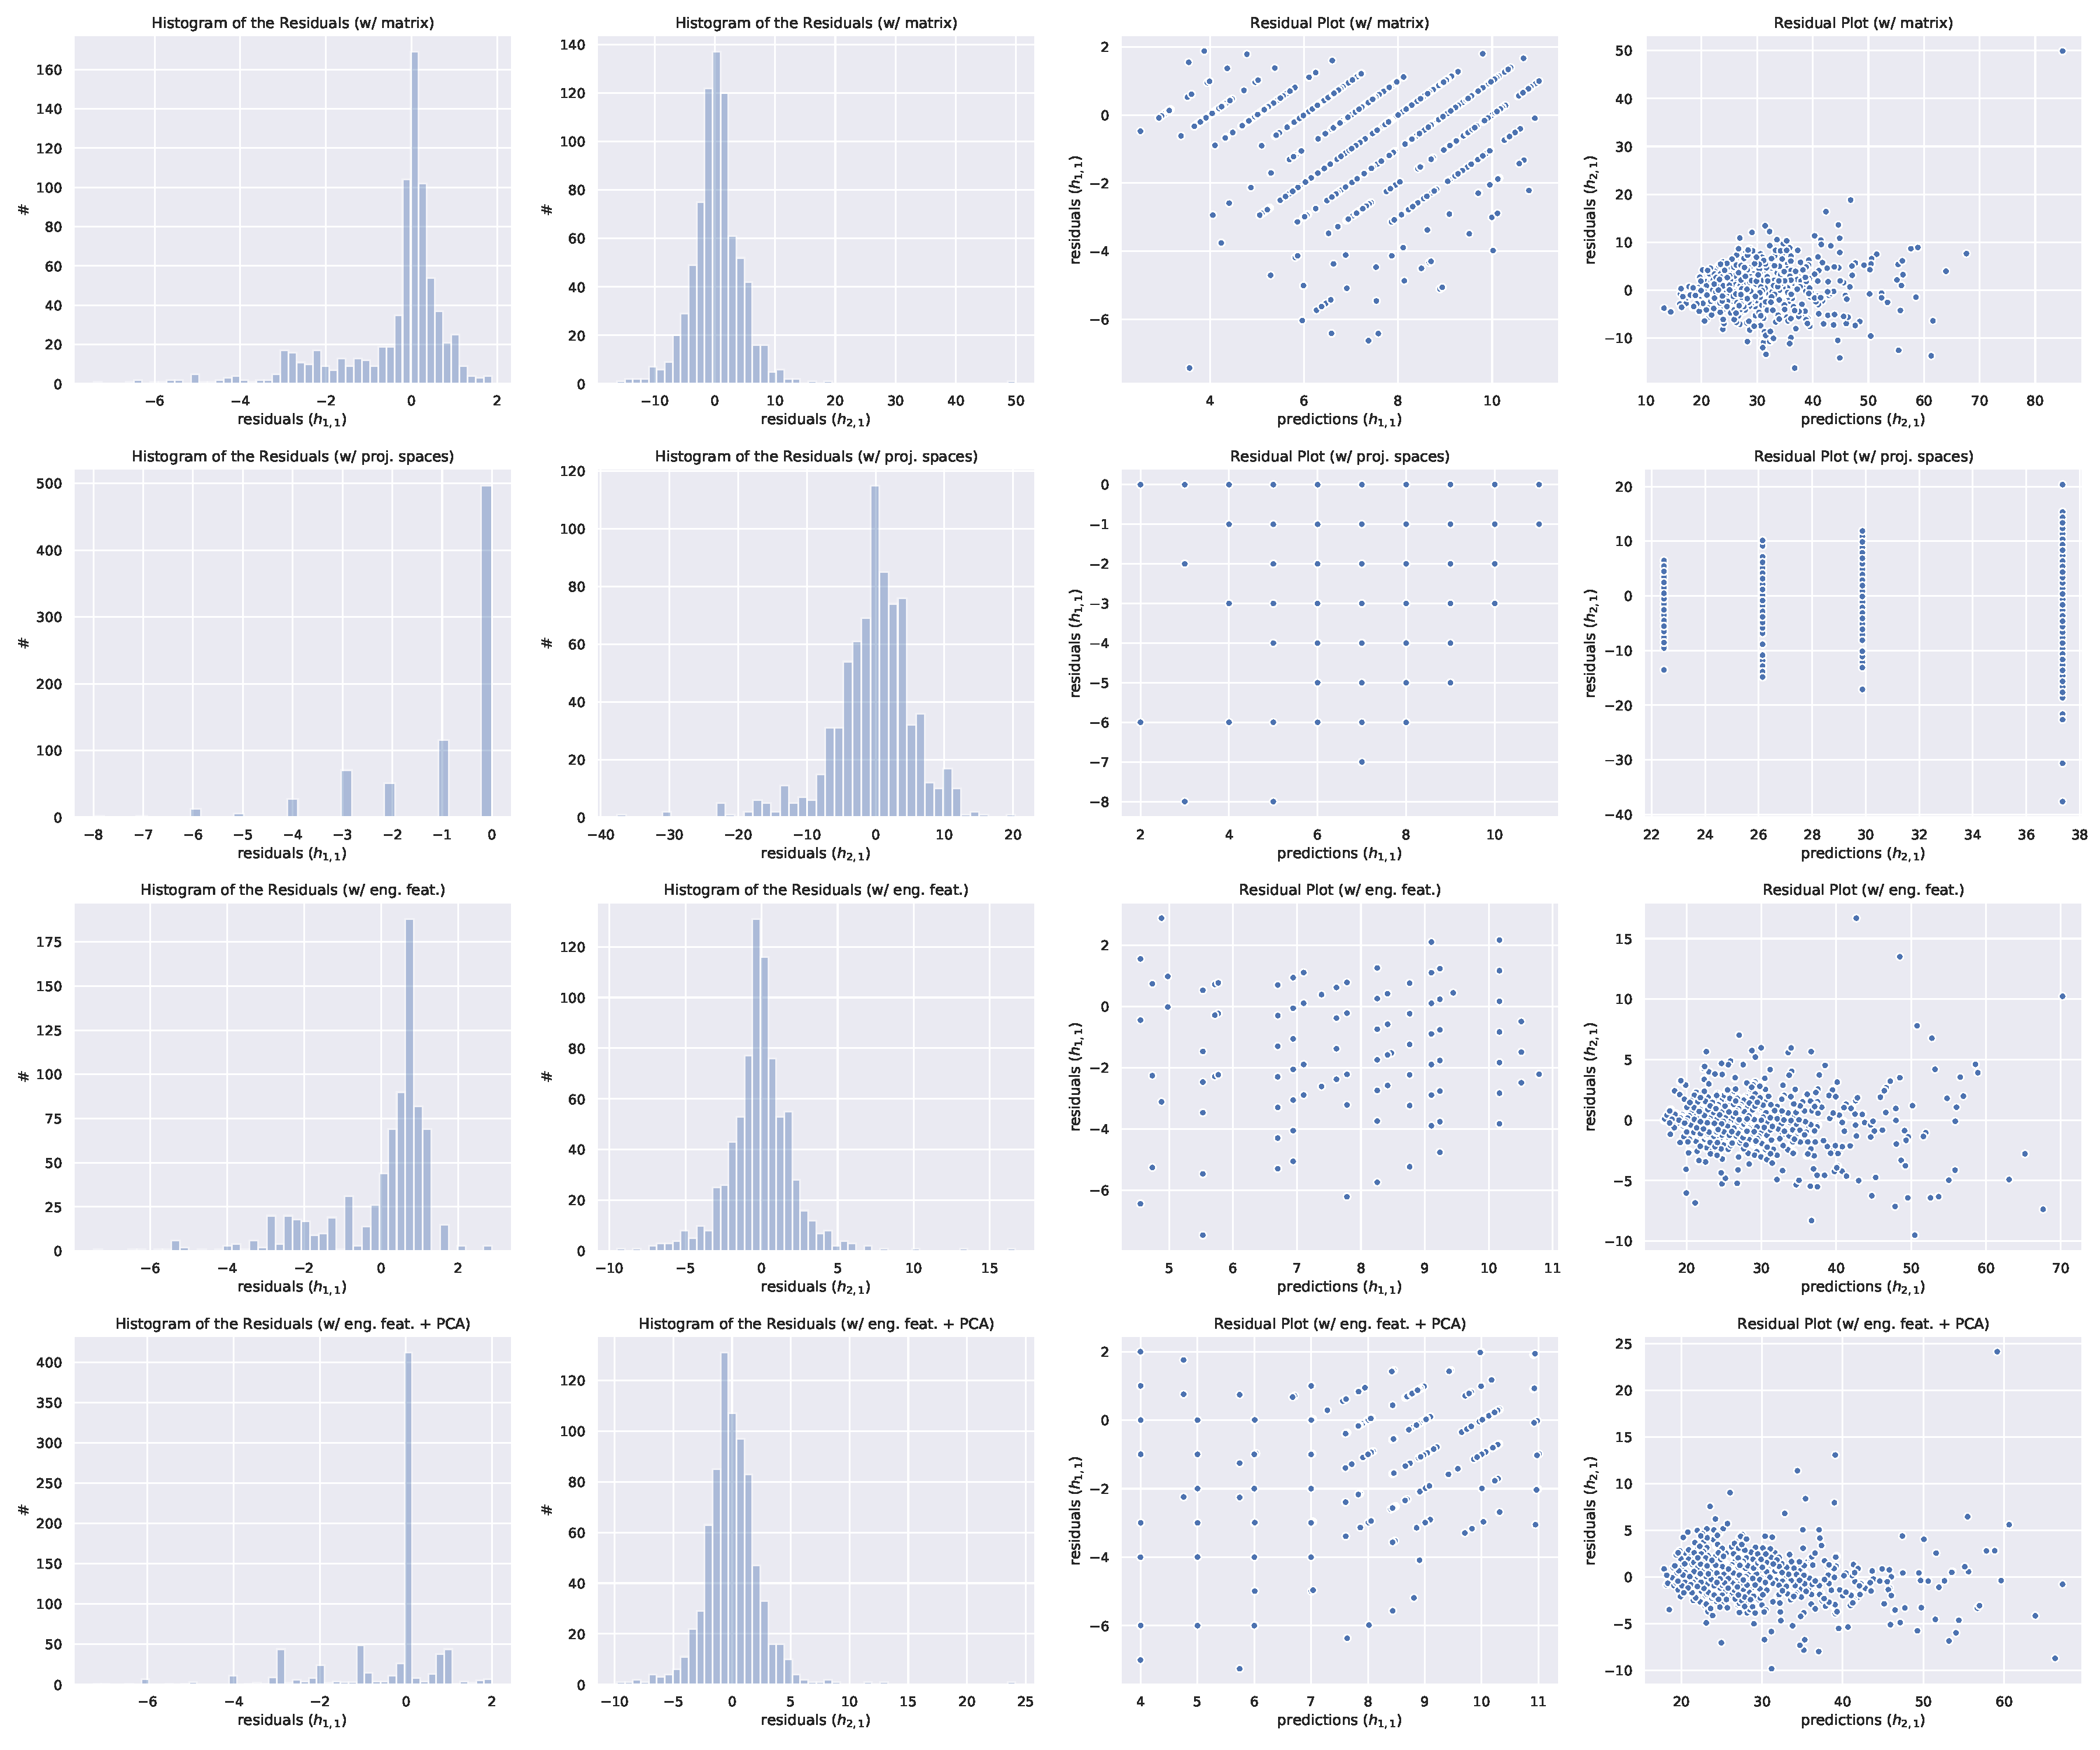
\includegraphics[width=0.9\linewidth]{img/grd_bst_orig}
  \caption{Plots of the residual errors for the gradient boosted trees.}
  \label{fig:res:grdbst}
\end{figure}


\subsection{Neural Networks}

In this section we approach the problem of predicting the Hodge numbers using artificial neural networks (\ann), which we briefly review in~\Cref{sec:app:nn}.
We use Google's \emph{Tensorflow} framework and \emph{Keras}, its high-level API, to implement the architectures and train the networks~\cite{Abadi:2015:TensorFlowLargescaleMachine}.
We explore different architectures and discuss the results.

Differently from the previous algorithms, we do not perform a cross-validation scoring but we simply retain \SI{10}{\percent} of the total set as a holdout validation set (also referred to as \emph{development} set) due to the computation power available.
Thus we use \SI{80}{\percent} of the samples for training, \SI{10}{\percent} for evaluation, and \SI{10}{\percent} as a test set.
For the same reason, the optimisation of the algorithm has been performed manually.

We always use the Adam optimiser with default learning rate \num{e-3} to perform the gradient descent and a fix batch size of $32$.
The network is trained for a large number of epochs to avoid missing possible local optima.
In order to avoid overshooting the minimum of the loss function, we dynamically reduce the learning rate both using the \emph{Adam} optimiser which implements learning rate decay, and through the callback \texttt{callbacks.ReduceLROnPlateau} in Keras, which scales the learning rate by a given factor when the monitored quantity (in our case the validation loss) does not decrease): we choose to reduce it by $0.3$ when the validation loss does not improve for at least $75$ epochs.
Moreover we stop training when the validation loss does not improve during $200$ epochs.
We then keep only the weights of the neural networks which gave the best results.
Batch normalisation layers are used with a momentum of $0.99$.
Training and evaluation were performed on a \texttt{NVidia GeForce 940MX} laptop GPU with \SI{2}{\giga\byte} of RAM memory.


\subsubsection{Fully Connected Network}

First we reproduce the analysis in~\cite{Bull:2018:MachineLearningCICY} for the prediction of \hodge{1}{1}.


\paragraph{Model}

The neural network presented in~\cite{Bull:2018:MachineLearningCICY} for the regression task contains $5$ hidden layers with $876$, $461$, $437$, $929$ and $404$ units (\Cref{fig:nn:dense}).
All layers (including the output layer) are followed by a ReLU activation and by a dropout layer with a rate of \num{0.2072}.
This network contains roughly \num{1.58e6} parameters.

The other hyperparameters (like the optimiser, batch size, number of epochs, regularisation, etc.) are not mentioned.
In order to reproduce the results, we fill the gap as follows:
\begin{itemize}
    \item Adam optimiser with batch size of $32$;
    
    \item maximal number epochs of $2000$ without early stopping;\footnote{It took around 20 minutes to train the model.}
    
    \item we implement learning rate reduction by $0.3$ after $75$ epochs without improvement of the validation loss;
    
    \item no $\ell_1$ or $\ell_2$ regularisation;
    
    \item a batch normalisation layer~\cite{Ioffe:2015:BatchNormalizationAccelerating} after each fully connected layer.
\end{itemize}


\paragraph{Results}

We reproduce the results from~\cite{Bull:2018:MachineLearningCICY}, which are summarised in~\Cref{tab:res:neuralnet-bull}.
The training process was very quick and the loss function is reported in~\Cref{fig:nn:bull_et_al_loss}.
We obtain an accuracy of \SI{77}{\percent} both on the development and the test set of the original dataset with \SI{80}{\percent} of training data (see \Cref{tab:res:ann}).
Using the same network we also achieve \SI{97}{\percent} of accuracy in the favourable dataset.

\begin{figure}[tbp]
  \centering
  \begin{subfigure}[c]{0.475\linewidth}
    \centering
    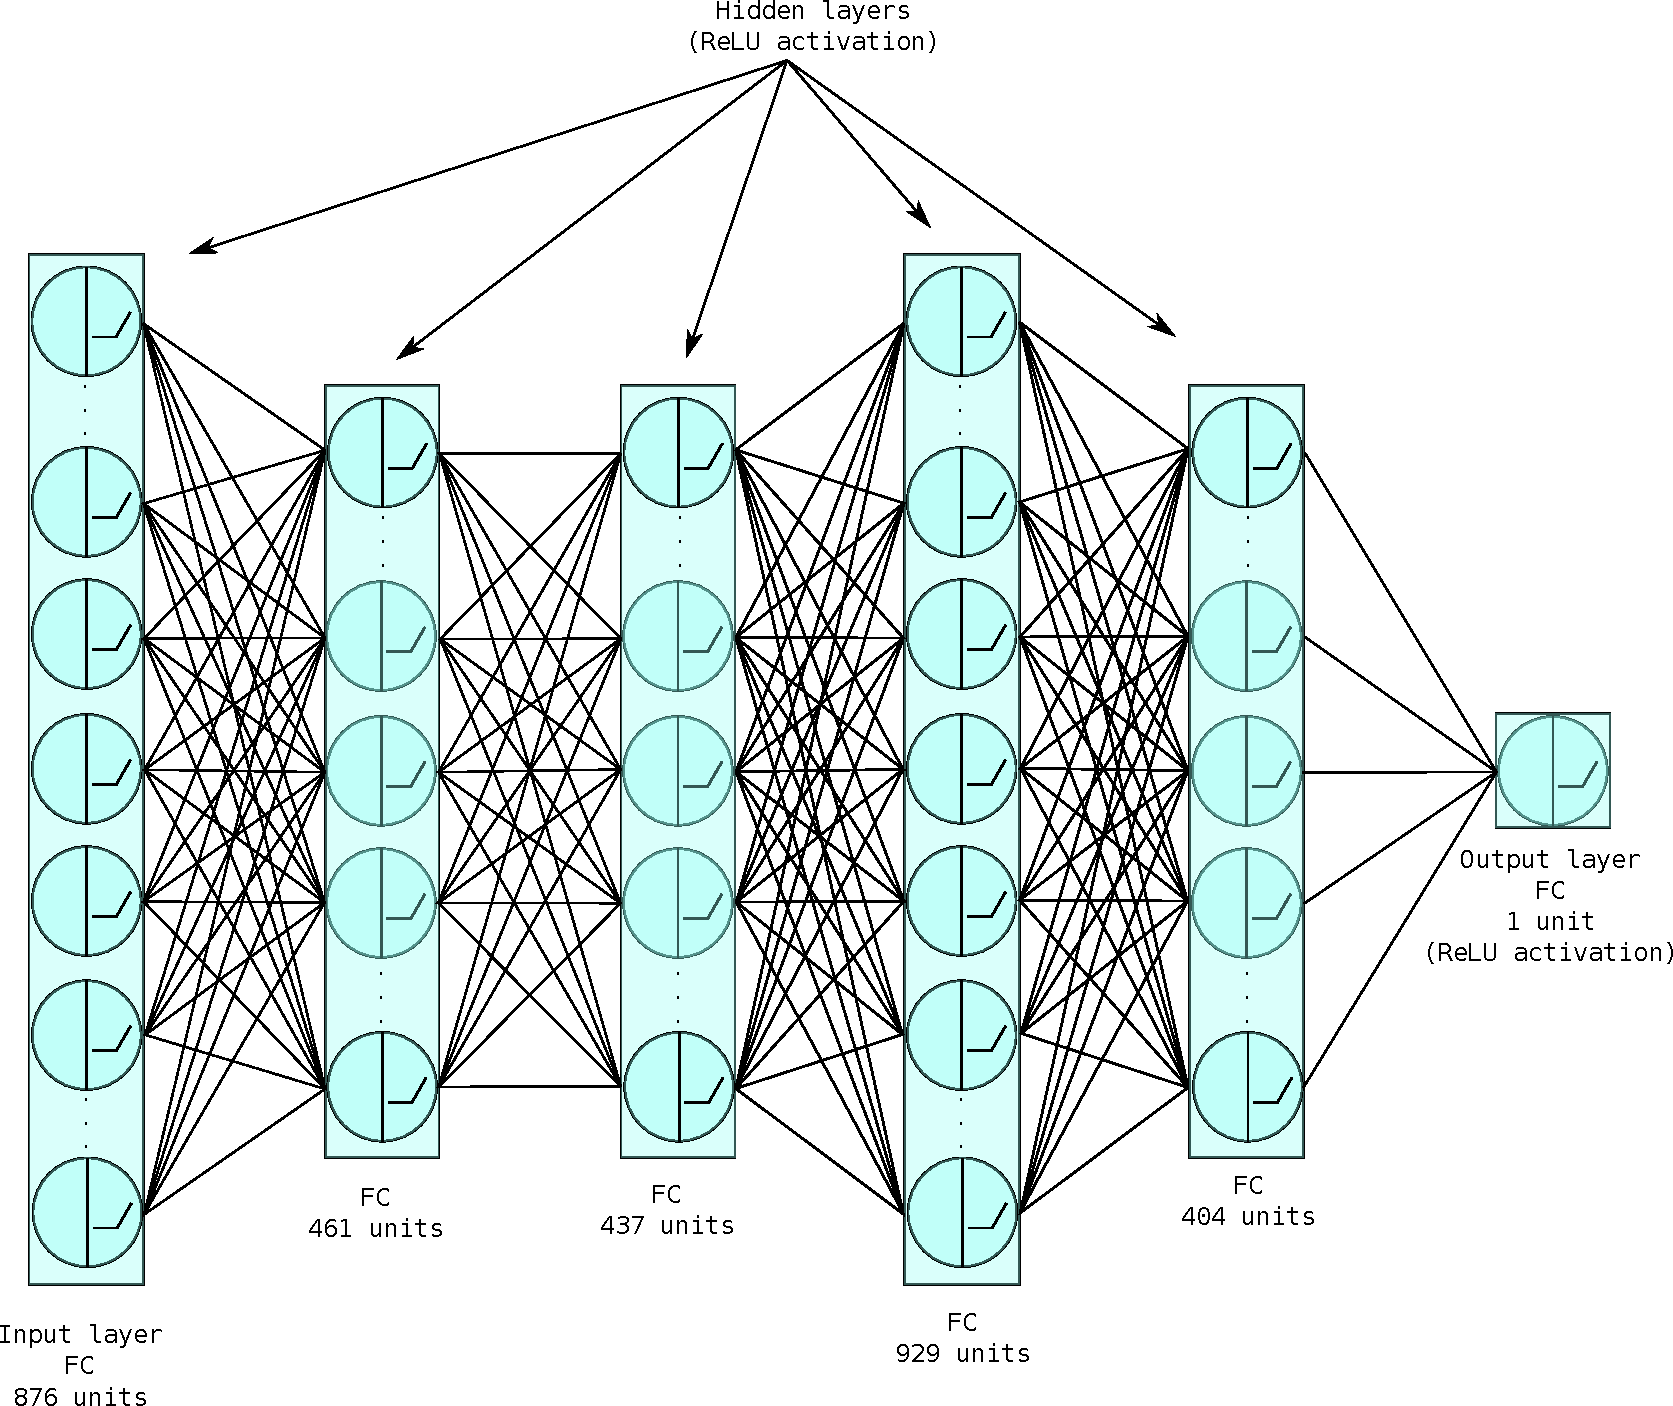
\includegraphics[width=\linewidth]{img/fc}
    \caption{Architecture of the network.}
    \label{fig:nn:dense}
  \end{subfigure}
  \hfill
  \begin{subfigure}[c]{0.475\linewidth}
    \centering
    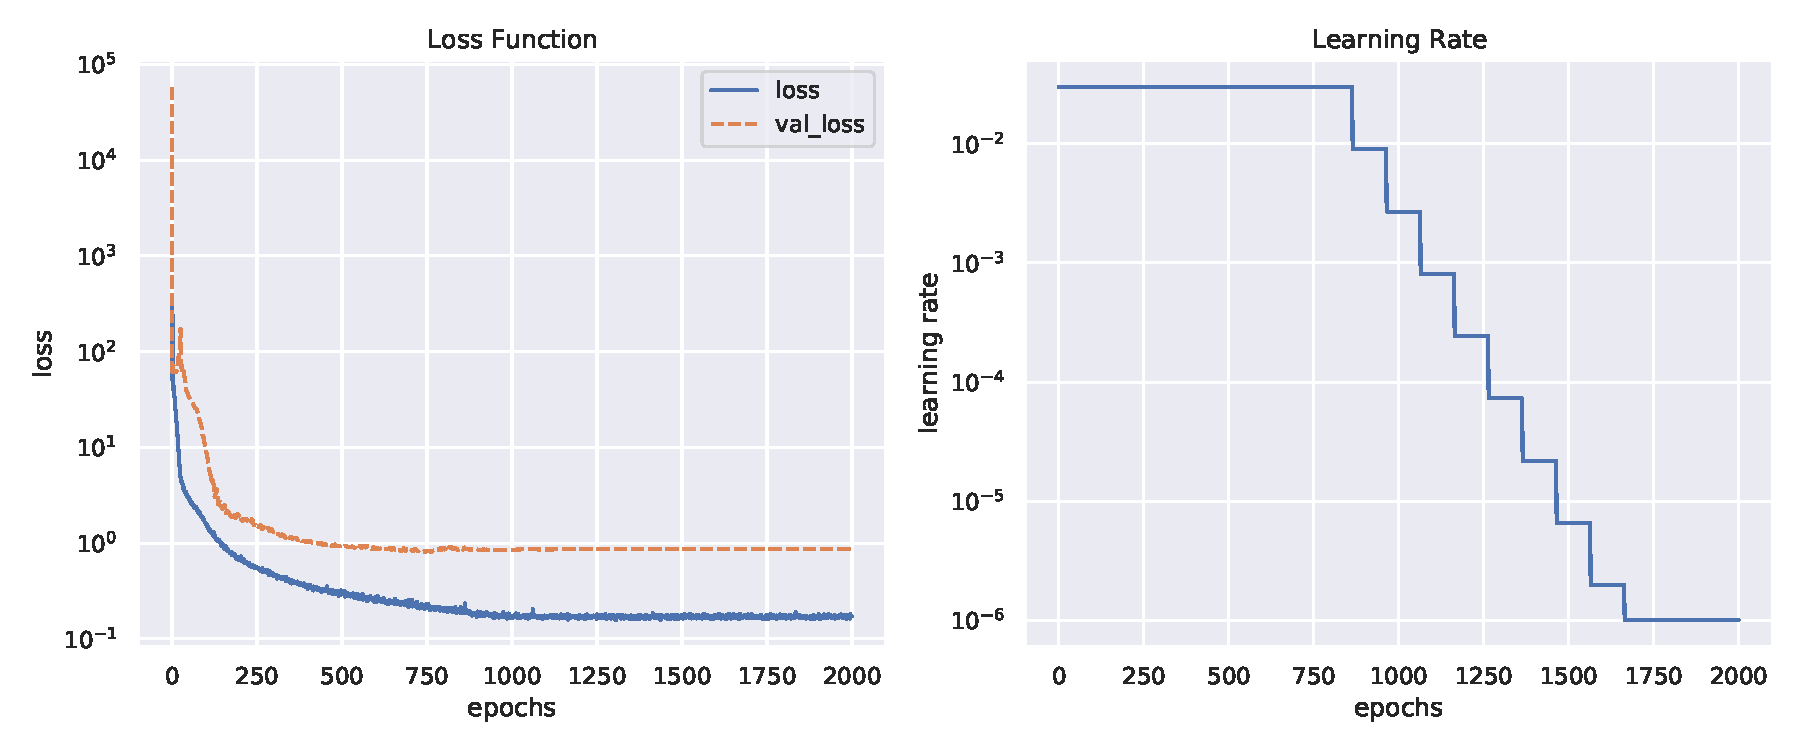
\includegraphics[width=\linewidth, trim={0 0 6in 0}, clip]{img/loss-lr_fc_orig}
    \caption{Loss function on the original dataset.}
    \label{fig:nn:bull_et_al_loss}
  \end{subfigure}
  \caption{%
    Fully connected network for the prediction of \hodge{1}{1}.
    For simplicity we do not draw the dropout and batch normalisation layers present after every densely connected layer.
  }
  \label{fig:nn:fcnetwork}
\end{figure}

\begin{table}[tbp]
  \centering
  \begin{tabular}{@{}cccccc@{}}
      \toprule
      &
      \multicolumn{5}{c}{\textbf{training data}}
      \\
          &
              \SI{10}{\percent} &
              \SI{30}{\percent} &
              \SI{50}{\percent} &
              \SI{70}{\percent} &
              \SI{90}{\percent}
          \\
          \midrule
          regression &
                  \SI{58}{\percent} &
                  \SI{68}{\percent} &
                  \SI{72}{\percent} &
                  \SI{75}{\percent} &
                  \SI{75}{\percent}
          \\
          classification &
                  \SI{68}{\percent} &
                  \SI{78}{\percent} &
                  \SI{82}{\percent} &
                  \SI{85}{\percent} &
                  \SI{88}{\percent}
          \\
          \bottomrule
  \end{tabular}
  \caption{Accuracy (approximate) for \hodge{1}{1} obtained in \cite[Figure~1]{Bull:2018:MachineLearningCICY}.}
  \label{tab:res:neuralnet-bull}
\end{table}


\subsubsection{Convolutional Network}

We then present a new purely convolutional neural network (\cnn) to predict \hodge{1}{1} and \hodge{2}{1}, separately or together.
The advantage of such networks is that it requires a smaller number of parameters and is insensitive to the size of the inputs.
The latter point can help to work without padding the matrices (of the same or different representations), but the use of a flatten layer removes this benefit.


\paragraph{Model}

The neural network has $4$ convolutional layers.
They are connected to the output layer with a intermediate flatten layer.
After each convolutional layer, we use the ReLU activation function and a batch normalisation layer (with momentum $0.99$).
Convolutional layers use the padding option \texttt{same} and a kernel of size $(5, 5)$ to be able to extract more meaningful representations of the input, treating the configuration matrix somewhat similarly to an object segmentation task~\cite{Peng:2017:LargeKernelMattersa}.
The output layer is also followed by a ReLU activation in order to force the prediction to be a positive number.
We use a dropout layer only after the convolutional network (before the flatten layer) but we introduced a combination of $\ell_2$ and $\ell_1$ regularisation to reduce the variance.
The dropout rate is $0.2$ in the original dataset and $0.4$ for the favourable dataset, while $\ell_1$ and $\ell_2$ regularisation are set to $10^{-5}$.
We train the model using the \emph{Adam} optimiser with a starting learning rate of $10^{-3}$ and a mini-batch size of $32$.

The architecture is more similar in style to the old \emph{LeNet} presented for the first time in 1998 by Y.\ LeCun during the ImageNet competition.
In our implementation however we do not include the pooling operations and swap the usual order of batch normalisation and activation function by first putting the ReLU activation.
In~\Cref{fig:nn:lenet} we show the model architecture in the case of the original dataset and of predicting \hodge{1}{1} alone.
The convolution layers have $180$, $100$, $40$ and $20$ units each.

\begin{figure}[tbp]
  \centering
  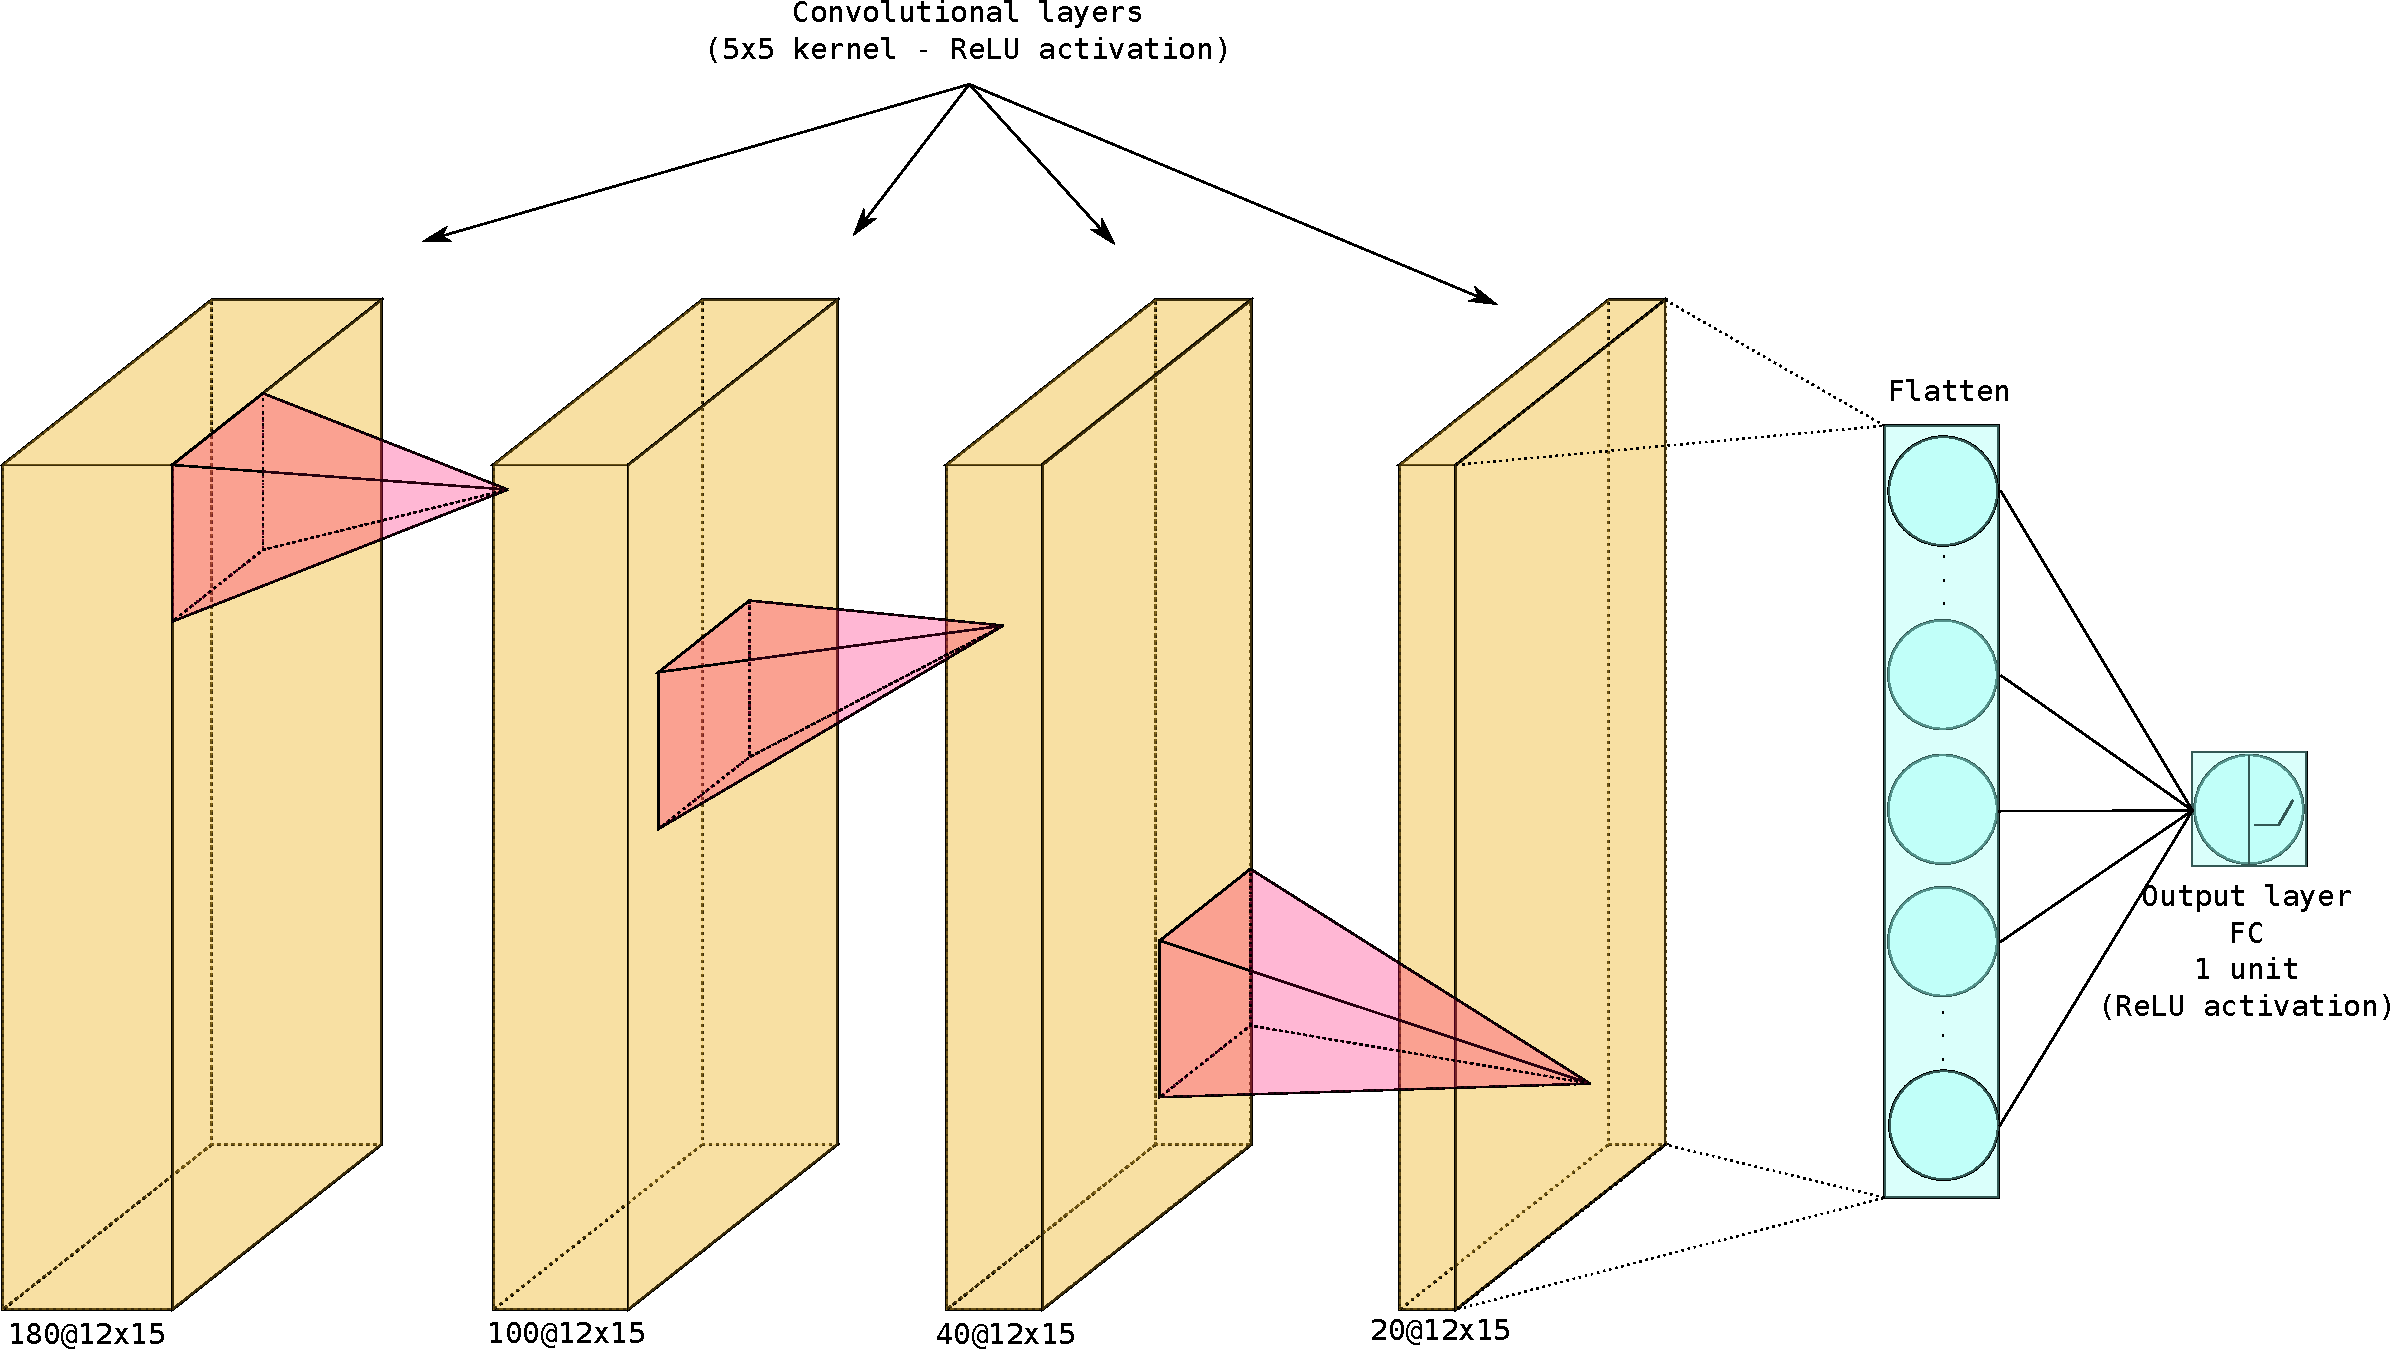
\includegraphics[width=0.75\linewidth]{img/ccnn}
  \caption{%
    Pure convolutional neural network for redicting \hodge{1}{1}.
    It is made of $4$ modules composed by convolutional layer, ReLU activation, batch normalisation (in this order), followed by a dropout layer, a flatten layer and the output layer (in this order).
  }
  \label{fig:nn:lenet}
\end{figure}


\paragraph{Results}

With this setup, we were able to achieve an accuracy of \SI{94}{\percent} on both the development and the test sets for the ``old'' database and \SI{99}{\percent} for the favourable dataset in both validation and test sets (results are briefly summarised in \Cref{tab:res:ann}).
We thus improved the results of the densely connected network and proved that convolutional networks can be valuable assets when dealing with the extraction of a good representation of the input data: not only are convolutional networks very good at recognising patterns and rotationally invariant objects inside pictures or general matrices of data, but deep architectures are also capable of transforming the input using non linear transformations~\cite{Mallat:2016:UnderstandingDeepConvolutional} to create new patterns which can then be used for predictions.

Even though the convolution operation is very time consuming another advantage of \cnn is the extremely reduced number of parameters with respect to fully connected (\fc) networks.\footnotemark{}
\footnotetext{%
  It took around 4 hours of training (and no optimisation) for each Hodge number in each dataset.
  The use use of modern generation GPUs with tensor cores can however speed up the training by order of magnitudes.
}
The architectures we used were in fact made of approximately \num{5.8e5} parameters: way less than half the number of parameters used in the \fc network.
Ultimately, this leads to a smaller number of training epochs necessary to achieve good predictions (see~\Cref{fig:cnn:class-ccnn}).

\begin{figure}[tbp]
  \centering
  \begin{subfigure}[c]{0.45\linewidth}
    \centering
    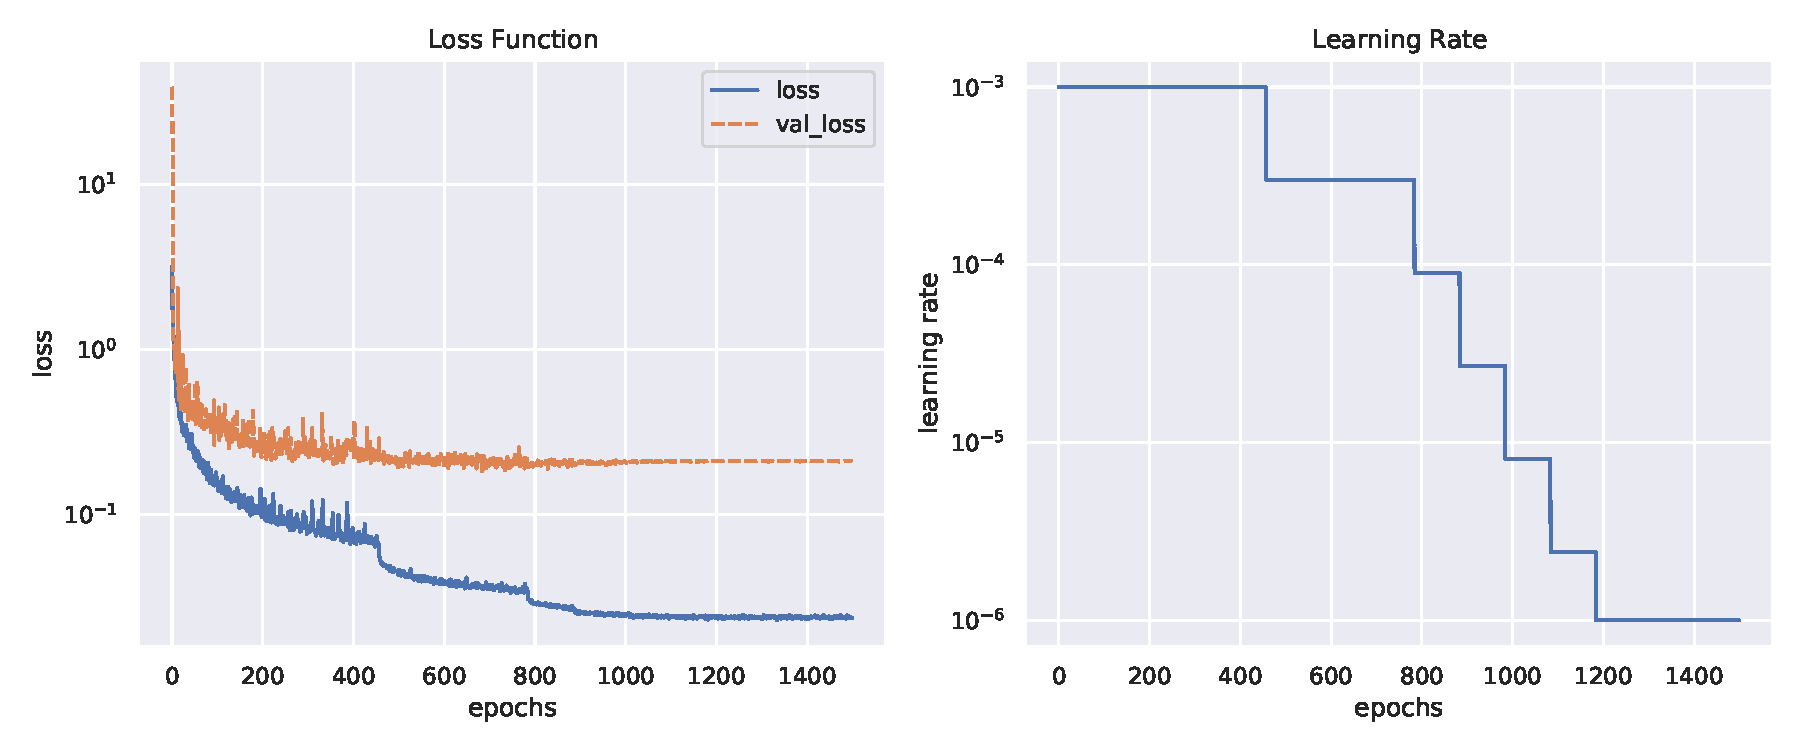
\includegraphics[width=\linewidth, trim={0 0 6in 0}, clip]{img/loss-lr_ccnn_h11_orig}
    \caption{Loss function of \hodge{1}{1}.}
  \end{subfigure}
  \hfill
  \begin{subfigure}[c]{0.45\linewidth}
    \centering
    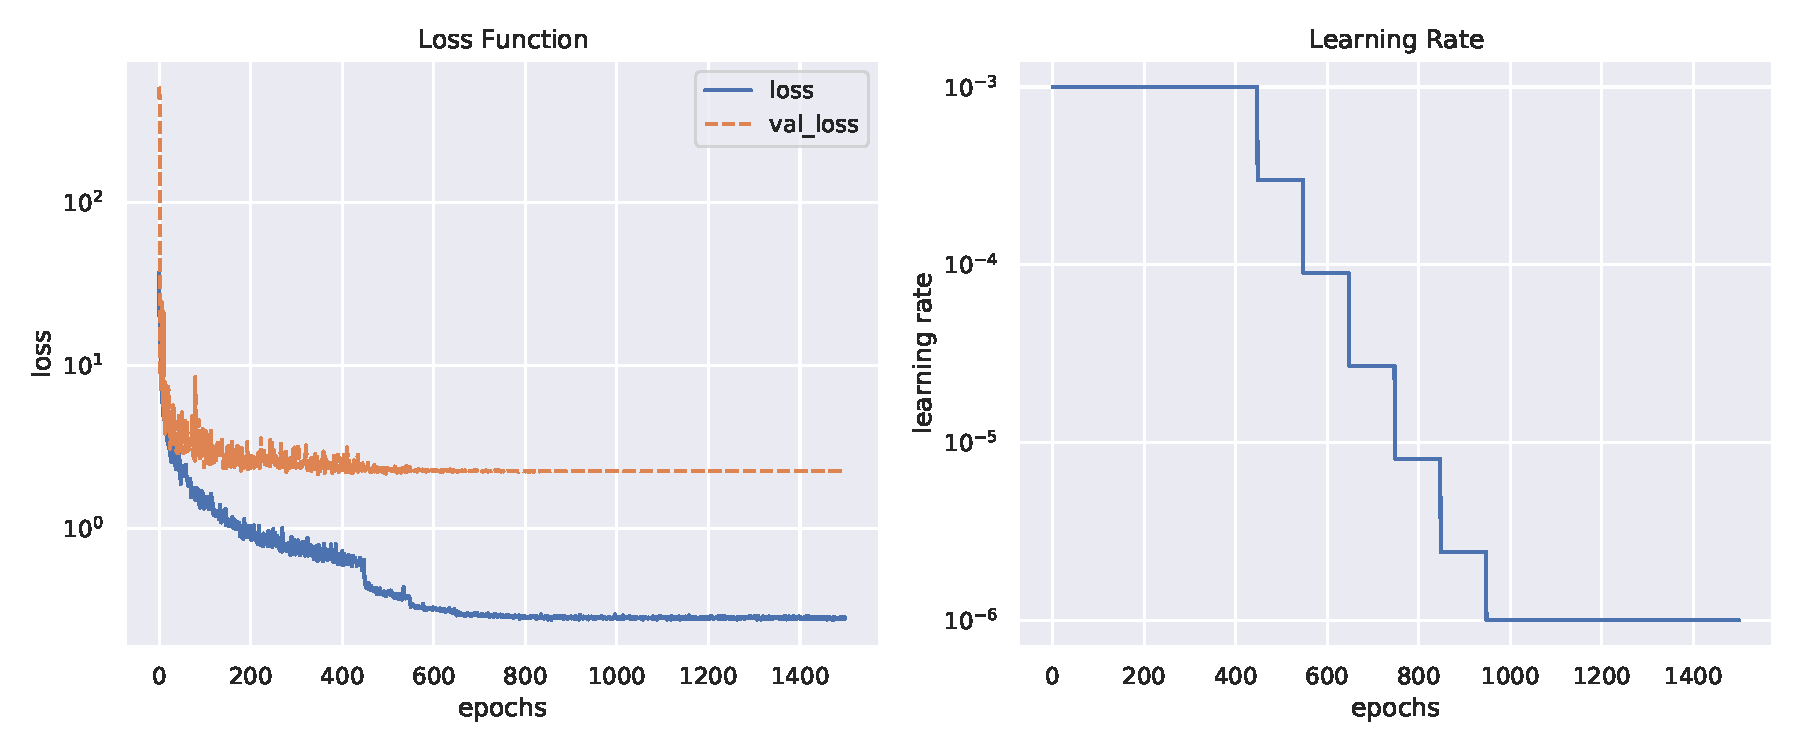
\includegraphics[width=\linewidth, trim={0 0 6in 0}, clip]{img/loss-lr_ccnn_h21_orig}
    \caption{Loss function of \hodge{2}{1}.}
  \end{subfigure}
  \caption{%
    Loss function of the networks for the prediction of \hodge{1}{1} and \hodge{2}{1}.
    We can see that the validation loss flattens out while the training loss keeps decreasing: we took care of the overfit by using the weights of the network when the validation loss reached its minimum.
    The use of mini-batch gradient descent also completely spoils the monotonicity of the loss functions which can therefore increase moving from one epoch to the other, while keeping the descending trend for most of its evolution.
  }
  \label{fig:cnn:class-ccnn}
\end{figure}

Using this classic setup we tried different architectures.
The network for the original dataset seems to work best in the presence of larger kernels, dropping by roughly \SI{5}{\percent} in accuracy when a more ``classical'' $3 \times 3$ kernel is used.
We also tried to use to set the padding to \texttt{valid}, reducing the input from a $12 \times 15$ matrix to a $1 \times 1$ feature map over the course of $5$ layers with $180$, $100$, $75$, $40$ and $20$ filters.
The advantage is the reduction of the number of parameters (namely $\sim \num{4.9e5}$) mainly due to the small \fc network at the end, but accuracy dropped to \SI{87}{\percent}.
The favourable dataset seems instead to be more independent of the specific architecture retaining accuracy also with smaller kernels.

The analysis for \hodge{2}{1} follows the same prescriptions.
For both the original and favourable dataset, we opted for 4 convolutional layers with \numlist{250;150;100;50} filters and no \fc network for a total amount of \num{2.1e6} parameters.
In this scenario we were able to achieve \SI{36}{\percent} of accuracy in the development set and \SI{40}{\percent} on the test set for \hodge{2}{1} in the ``old'' dataset and \SI{31}{\percent} in both development and test sets in the favourable set (see~\Cref{tab:res:ann}).
The learning curves for both Hodge numbers are given in \Cref{fig:lc:class-ccnn}.
This model uses the same architecture as the one for predicting \hodge{1}{1} only, which explains why it is less accurate as it needs to also adapt to compute \hodge{2}{1} (see for example \Cref{fig:lc:inception}).

\begin{figure}[tbp]
  \centering
  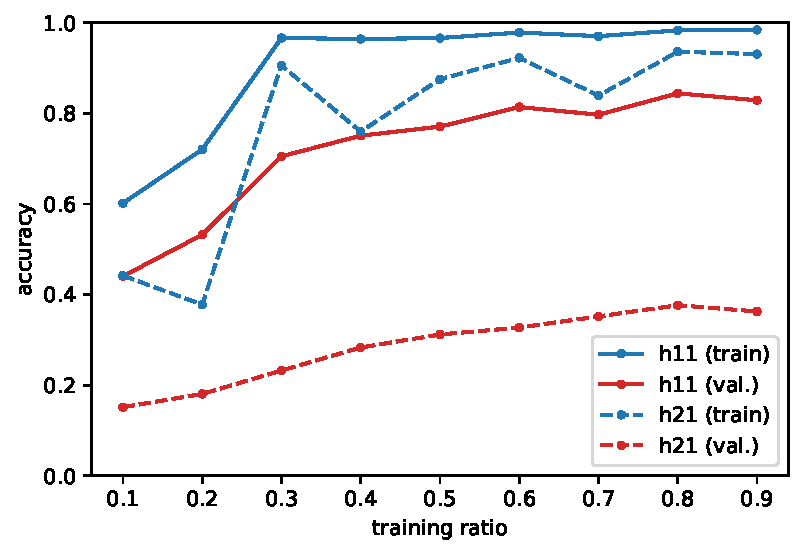
\includegraphics[width=0.6\linewidth]{img/conv_nn_learning_curve}
  \caption{%
    Learning curves for the classic convolutional neural network (original dataset), using a single model for both Hodge numbers.
  }
  \label{fig:lc:class-ccnn}
\end{figure}


\subsubsection{Inception-like Neural Network}
\label{sec:ml:nn:inception}

In the effort to find a better architecture, we took inspiration from Google's winning \cnn in the annual \href{https://image-net.org/challenges/LSVRC/}{\emph{ImageNet challenge}} in 2014~\cite{Szegedy:2015:GoingDeeperConvolutions, Szegedy:2016:RethinkingInceptionArchitecture, Szegedy:2016:Inceptionv4InceptionresnetImpact}.
The architecture in its original presentation uses \emph{inception} modules in which separate $1 \times 1$, $3 \times 3$ and  $5 \times 5$ convolutions are performed side by side (together with \emph{max pooling} operations) before recombining the outputs.
The modules are then repeated until the output layer is reached.
This has two evident advantages: users can avoid taking a completely arbitrary decision on the type of convolution to use since the network will take care of it tuning the weights, and the number of parameters is extremely restricted as the network can learn complicated functions using fewer layers.
As a consequence the architecture of such models can be made very deep while keeping the number of parameters contained, thus being able to learn very difficult representations of the input and producing accurate predictions.
Moreover while the training phase might become very long due to the complicated convolutional operations, the small number of parameters is such that predictions can be generated in a very small amount of time making inception-like models extremely appropriate whenever quick predictions are necessary.
Another advantage of the architecture is the presence of different kernel sizes inside each module: the network automatically learns features at different scales and different positions thus leveraging the advantages of a deep architecture with the ability to learn different representations at the same time and compare them.


\paragraph{Model}

In~\Cref{fig:nn:inception} we show a schematic of our implementation.
Differently from the image classification task, we drop the pooling operation and implement two side-by-side convolution over rows ($12 \times 1$ kernel for the original dataset, $15 \times 1$ for the favourable) and one over columns ($1 \times 15$ and $1 \times 18$ respectively).\footnotemark{}
\footnotetext{%
  Pooling operations are used to shrink the size of the input.
  Similar to convolutions, they use a window of a given size to scan the input and select particular values inside.
  For instance, we could select the average value inside the small portion selected, performing an \emph{average pooling} operation, or the maximum value, a \emph{max pooling} operation.
  This usually improves image classification and object detection tasks as it can be used to sharpen edges and borders.
}
We use \texttt{same} as padding option.
The output of the convolutions are then concatenated in the filter dimensions before repeating the ``inception'' module.
The results from the last module are directly connected to the output layer through a flatten layer.
In both datasets we use batch normalisation layers (with momentum $0.99$) after each concatenation layer and a dropout layer (with rate $0.2$) before the \fc network.\footnotemark{}
\footnotetext{%
  The position of the batch normalisation is extremely important as the parameters computed by such layer directly influence the following batch.
  We however opted to wait for the scan over rows and columns to finish before normalising the outcome to avoid biasing the resulting activation function.
}

For both \hodge{1}{1} and \hodge{2}{1} (in both datasets) we used 3 modules made by \numlist{32;64;32} filters for the first Hodge number, and \numlist{128;128;64} filters for the second.
We also included $\ell_1$ and $\ell_2$ regularisation of magnitude \num{e-4} in all cases.
The number of parameters was thus restricted to \num{2.3e5} parameters for \hodge{1}{1} in the original dataset and \num{2.9e5} in the favourable set, and \num{1.1e6} parameters for \hodge{2}{1} in the original dataset and \num{1.4e6} in the favourable dataset.
In all cases the number of parameters has decreased by a significant amount: in the case of \hodge{1}{1} they are roughly $\frac{1}{3}$ of the parameters used in the classical \cnn and around $\frac{1}{6}$ of those used in the \fc network.
During training we used the \emph{Adam} gradient descent with an initial learning rate of $10^{-3}$ and a batch size of $32$.
The callbacks helped to contain the training time (without optimisation) under 5 hours for each Hodge number in each dataset.

\begin{figure}[tbp]
  \centering
  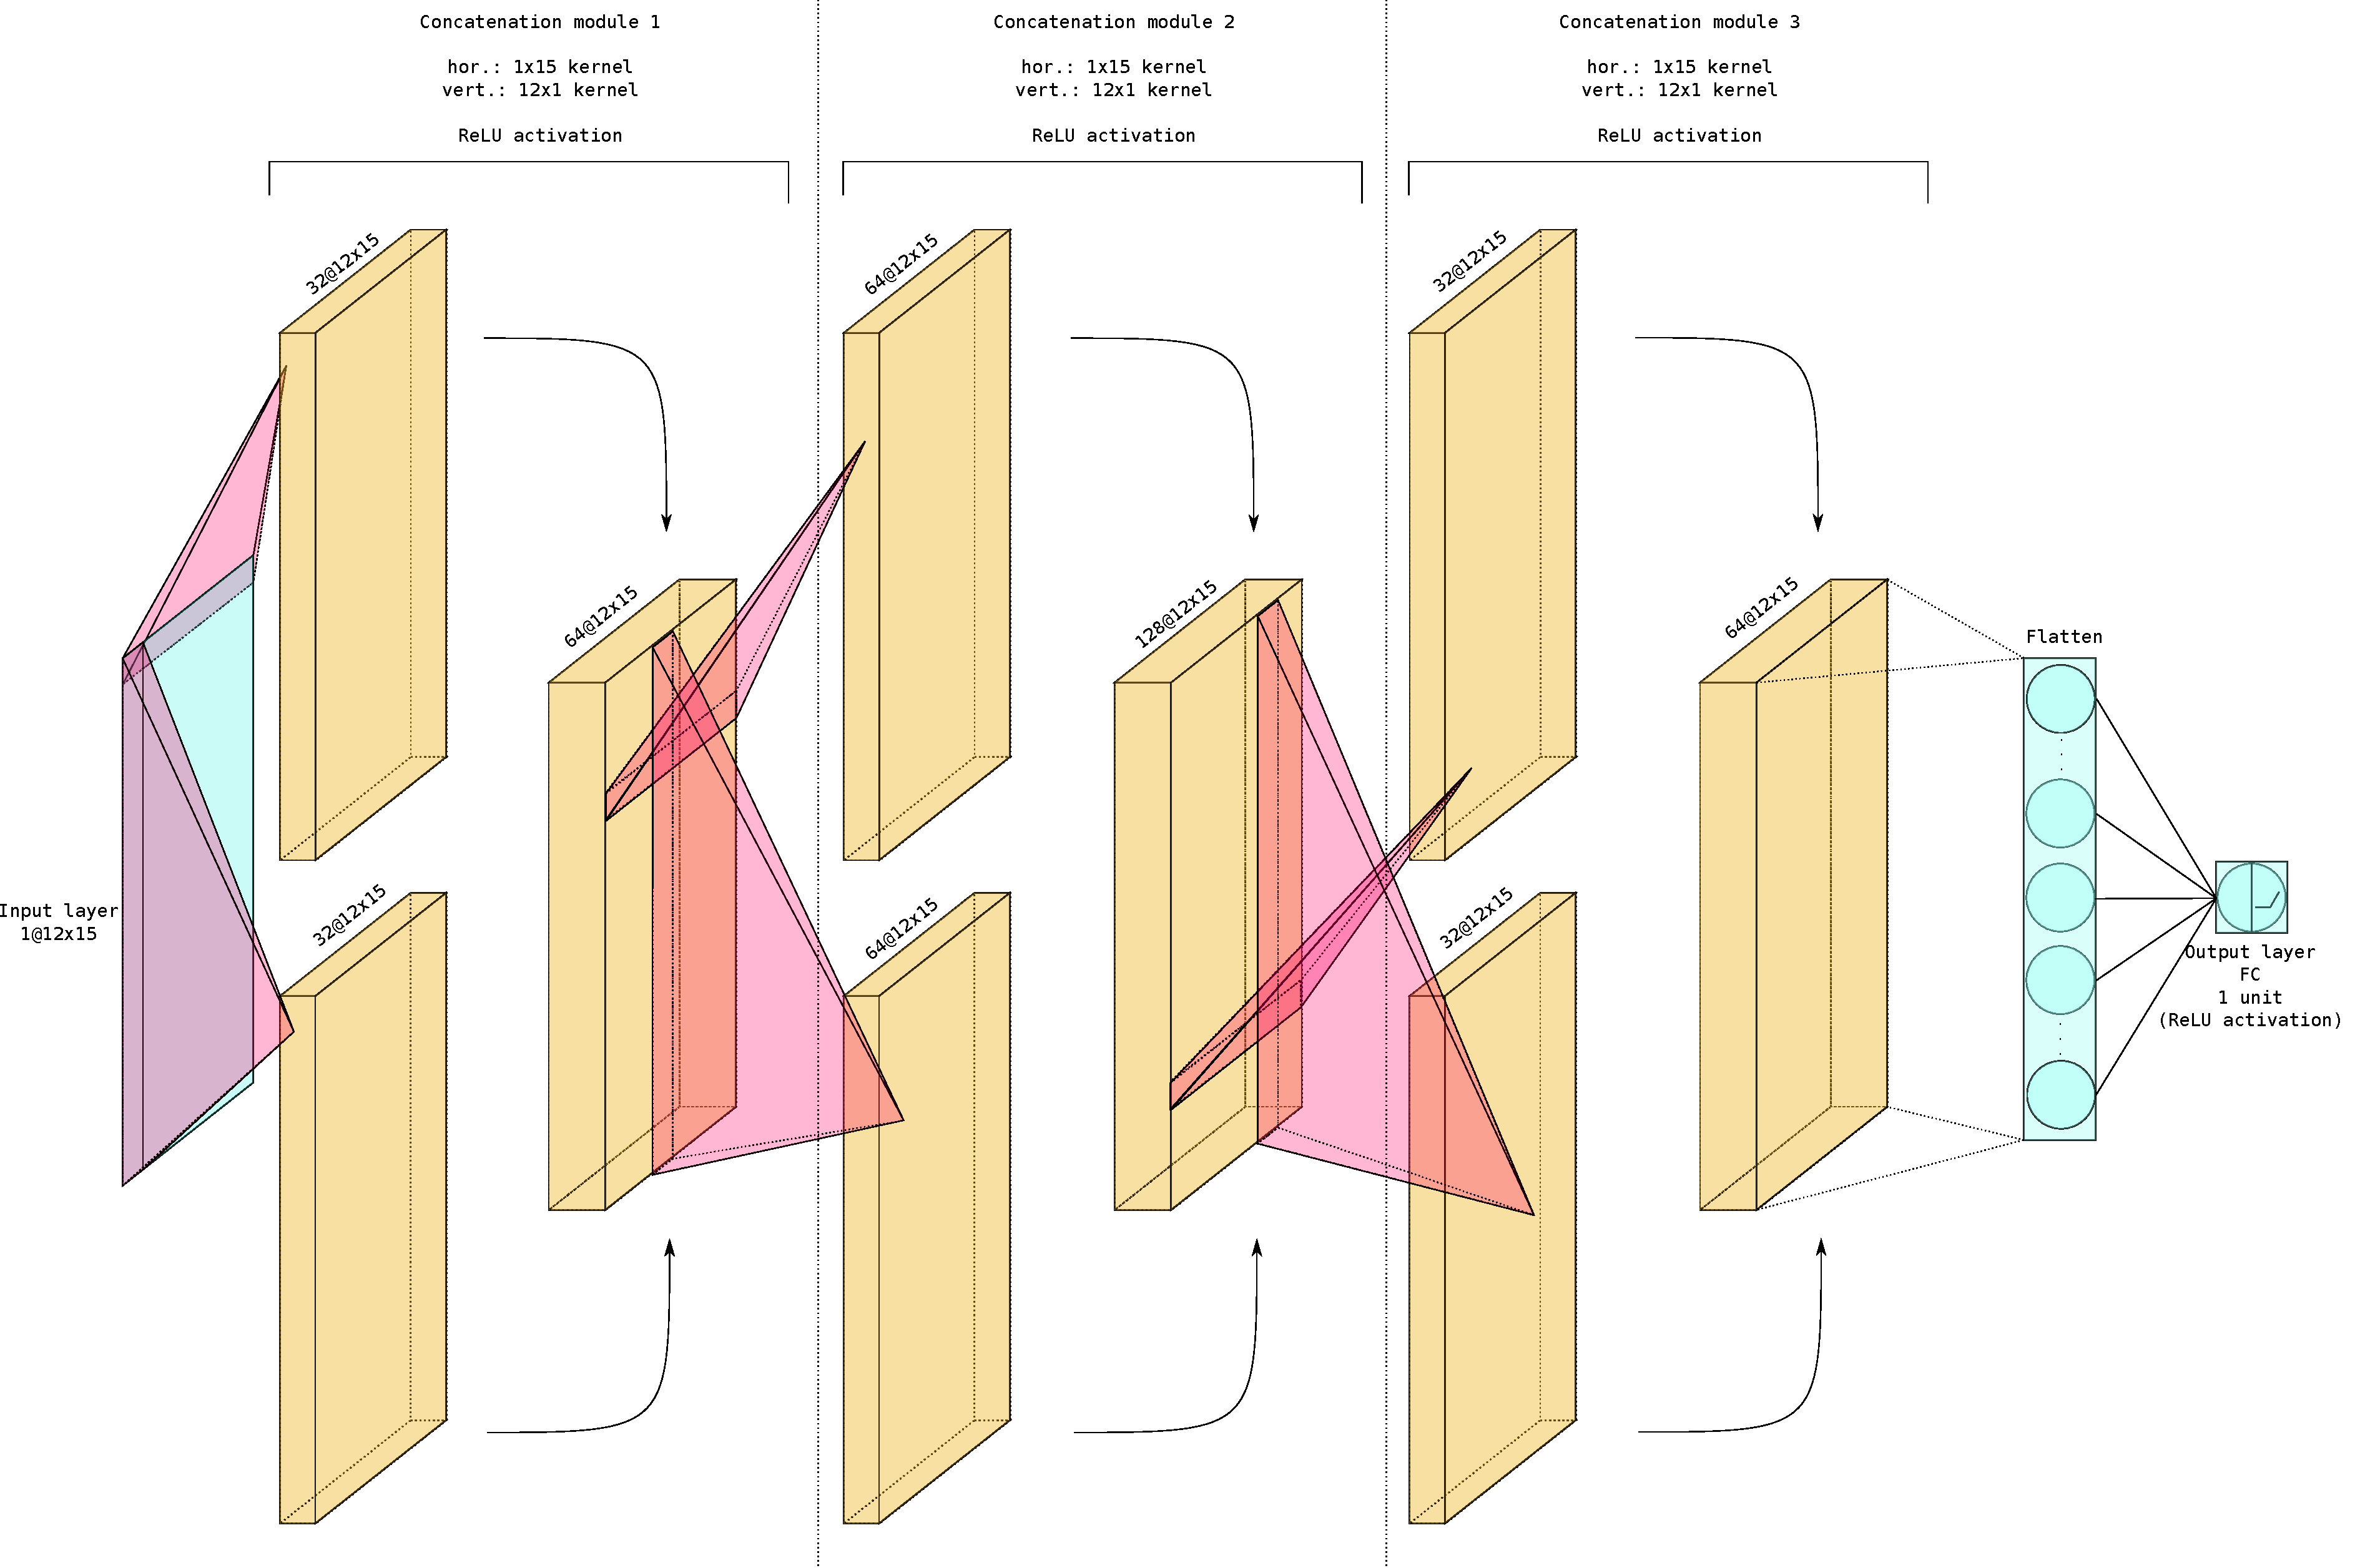
\includegraphics[width=0.9\linewidth]{img/icnn}
  \caption{%
    In each concatenation module (here shown for the ``old'' dataset) we operate with separate convolution operations over rows and columns, then concatenate the results.
    The overall architecture is composed of 3 ``inception'' modules made by two separate convolutions, a concatenation layer and a batch normalisation layer (strictly in this order), followed by a dropout layer, a flatten layer and the output layer with ReLU activation (in this order).
  }
  \label{fig:nn:inception}
\end{figure}


\paragraph{Results}

With these architectures we were able to achieve more than \SI{99}{\percent} of accuracy for \hodge{1}{1} in the test set (same for the development set) and \SI{50}{\percent} of accuracy for \hodge{2}{1} (a slightly smaller value for the development set).
We report the results in~\Cref{tab:res:ann}.

We therefore increased the accuracy for both Hodge numbers (especially \hodge{2}{1}) compared to what can achieve a simple sequential network, while at the same time reducing significantly the number of parameters of the network.\footnotemark{}
\footnotetext{%
  In an attempt to improve the results for \hodge{2}{1} even further, we also considered to first predict $\ln( 1 + \hodge{2}{1} )$ and then transform it back.
  However, the predictions dropped by almost \SI{10}{\percent} in accuracy even using the ``inception'' network: the network seems to be able to approximate quite well the results (not better nor worse than simply \hodge{2}{1}) but the subsequent exponentiation is taking apart predictions and true values.
  Choosing a correct rounding strategy then becomes almost impossible.
}
This increases the robustness of the method and its generalisation properties.

In~\Cref{fig:nn:inception_errors} we show the distribution of the residuals and their scatter plot.
The distribution of the errors does not present pathological behaviour and the variance of the residuals is well distributed over the predictions.
In fact this neural network is much more powerful than the previous networks we considered, as can be seen by studying the learning curves in~\Cref{fig:lc:inception}.
When predicting only \hodge{1}{1} it surpasses \SI{97}{\percent} accuracy using only \SI{30}{\percent} of the data for training.
While it seems that the predictions suffer when using a single network for both Hodge numbers this remains much better than any other algorithm.
It may seem counter-intuitive that convolutions work well on this data since they are not translation or rotation invariant but only permutation invariant.
However convolution alone is not sufficient to ensure invariances under these transformations but it must be supplemented with pooling operations~\cite{Bengio:2017:DeepLearning} which we do not use.
Moreover convolution layers do more than just taking translation properties into account: they allow to make highly complicated combinations of the inputs and to share weights among components to find subtler patterns than standard fully connected layers.
This network is more studied in more details in~\cite{Erbin:2020:InceptionNeuralNetwork}.

\begin{figure}[tbp]
  \centering
  \begin{subfigure}[c]{0.45\linewidth}
    \centering
    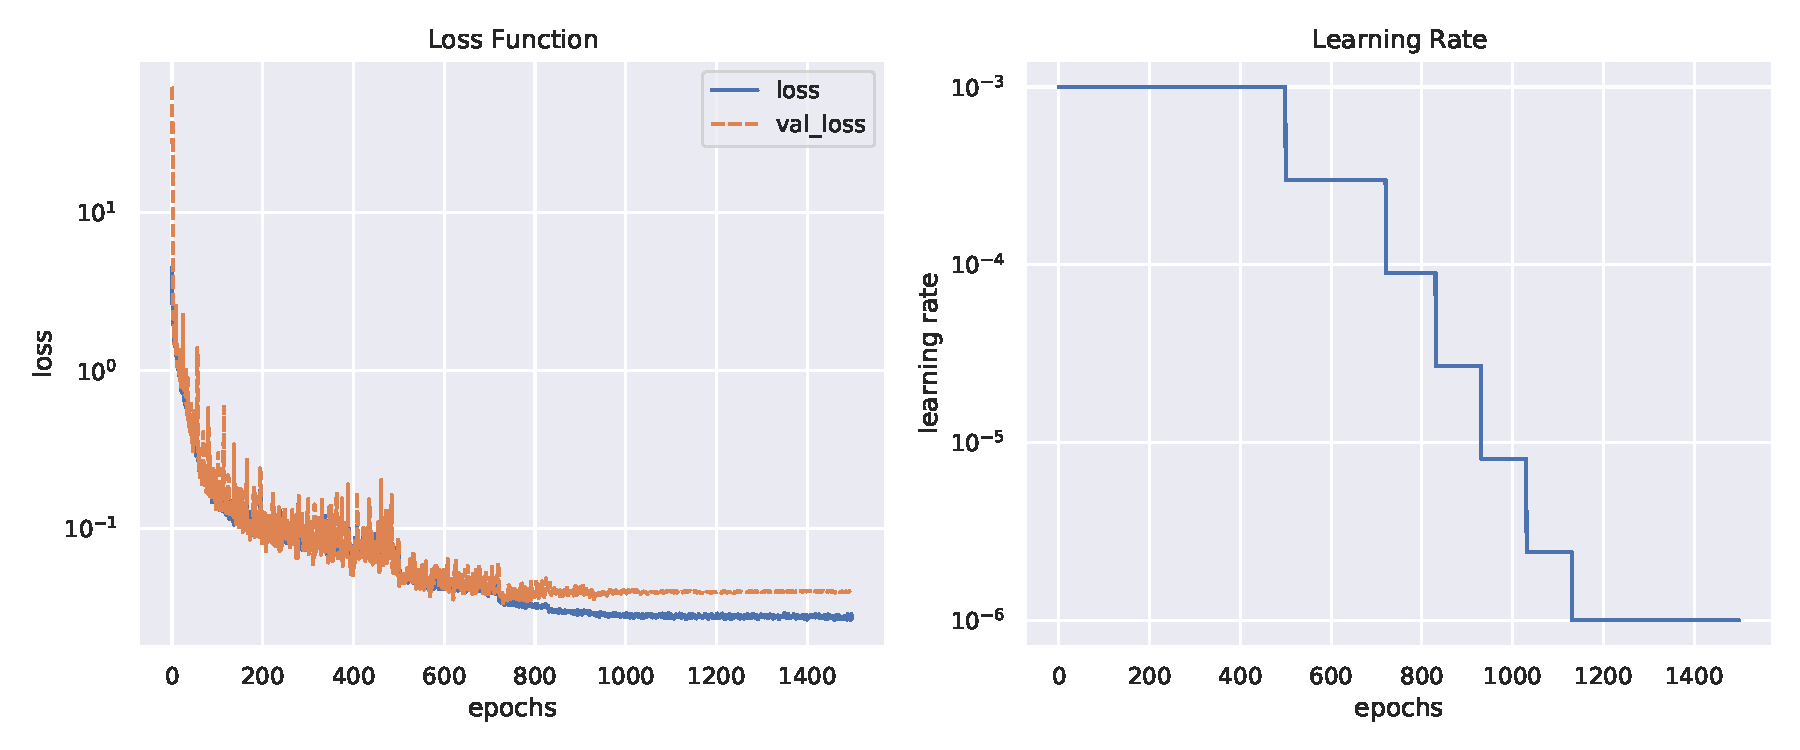
\includegraphics[width=\linewidth, trim={0 0 6in 0}, clip]{img/loss-lr_icnn_h11_orig}
    \caption{Loss of \hodge{1}{1}.}
  \end{subfigure}
  \quad
  \begin{subfigure}[c]{0.45\linewidth}
    \centering
    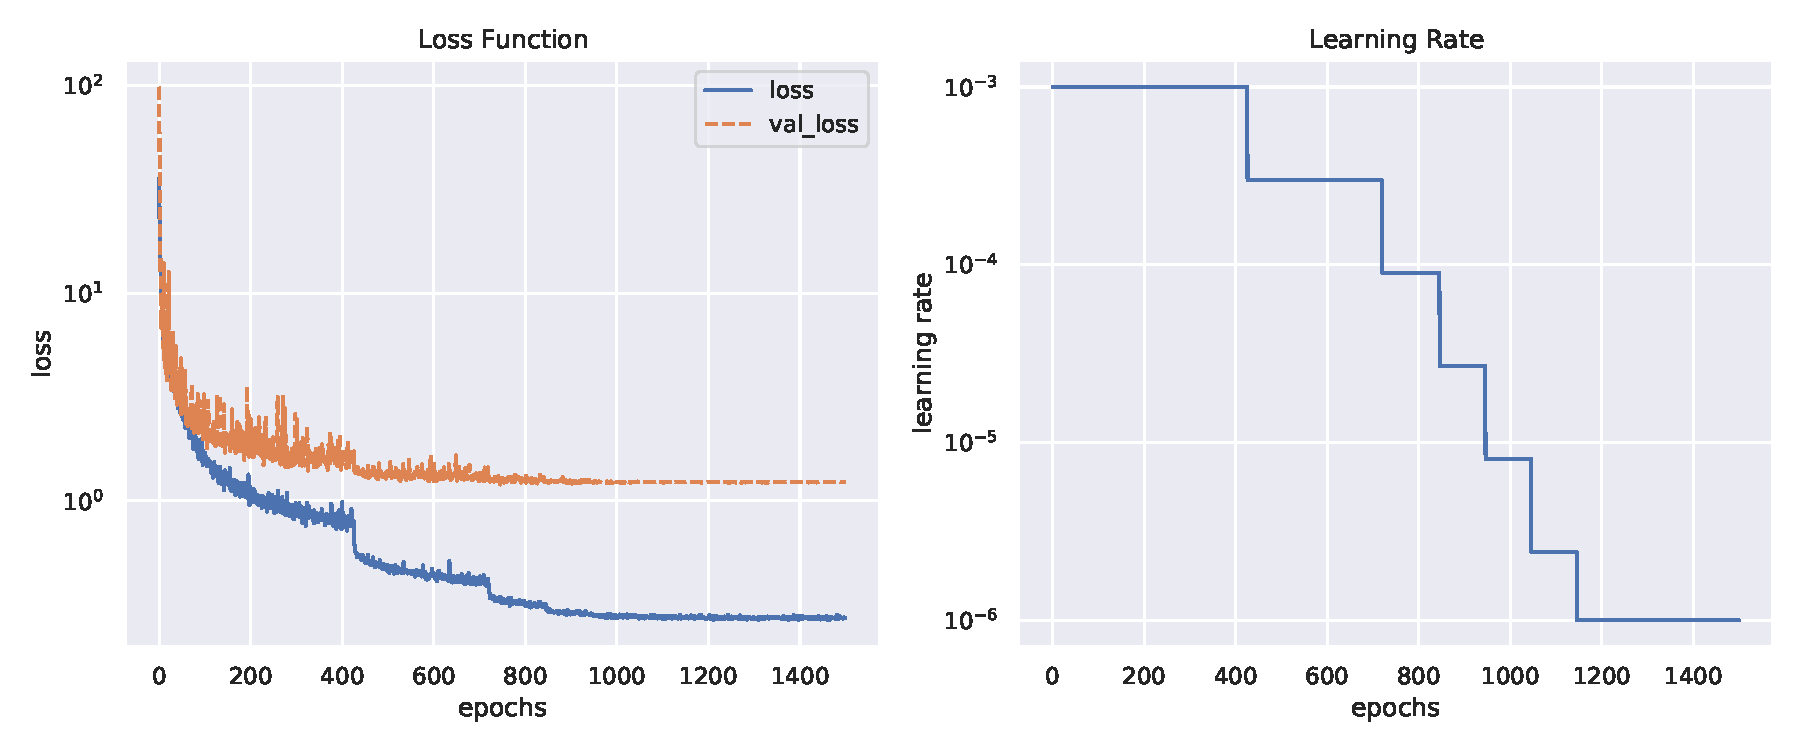
\includegraphics[width=\linewidth, trim={0 0 6in 0}, clip]{img/loss-lr_icnn_h21_orig}
    \caption{Loss of \hodge{2}{1}.}
  \end{subfigure}
  \caption{%
    The loss functions of ``inception'' network for \hodge{1}{1} and \hodge{2}{1} in the original dataset show that the number of epochs required for training is definitely larger than for simpler architectures, despite the reduced number of parameters.
  }
  \label{fig:cnn:inception-loss}
\end{figure}

\begin{figure}[tbp]
  \centering
  \begin{subfigure}[c]{\linewidth}
    \centering
    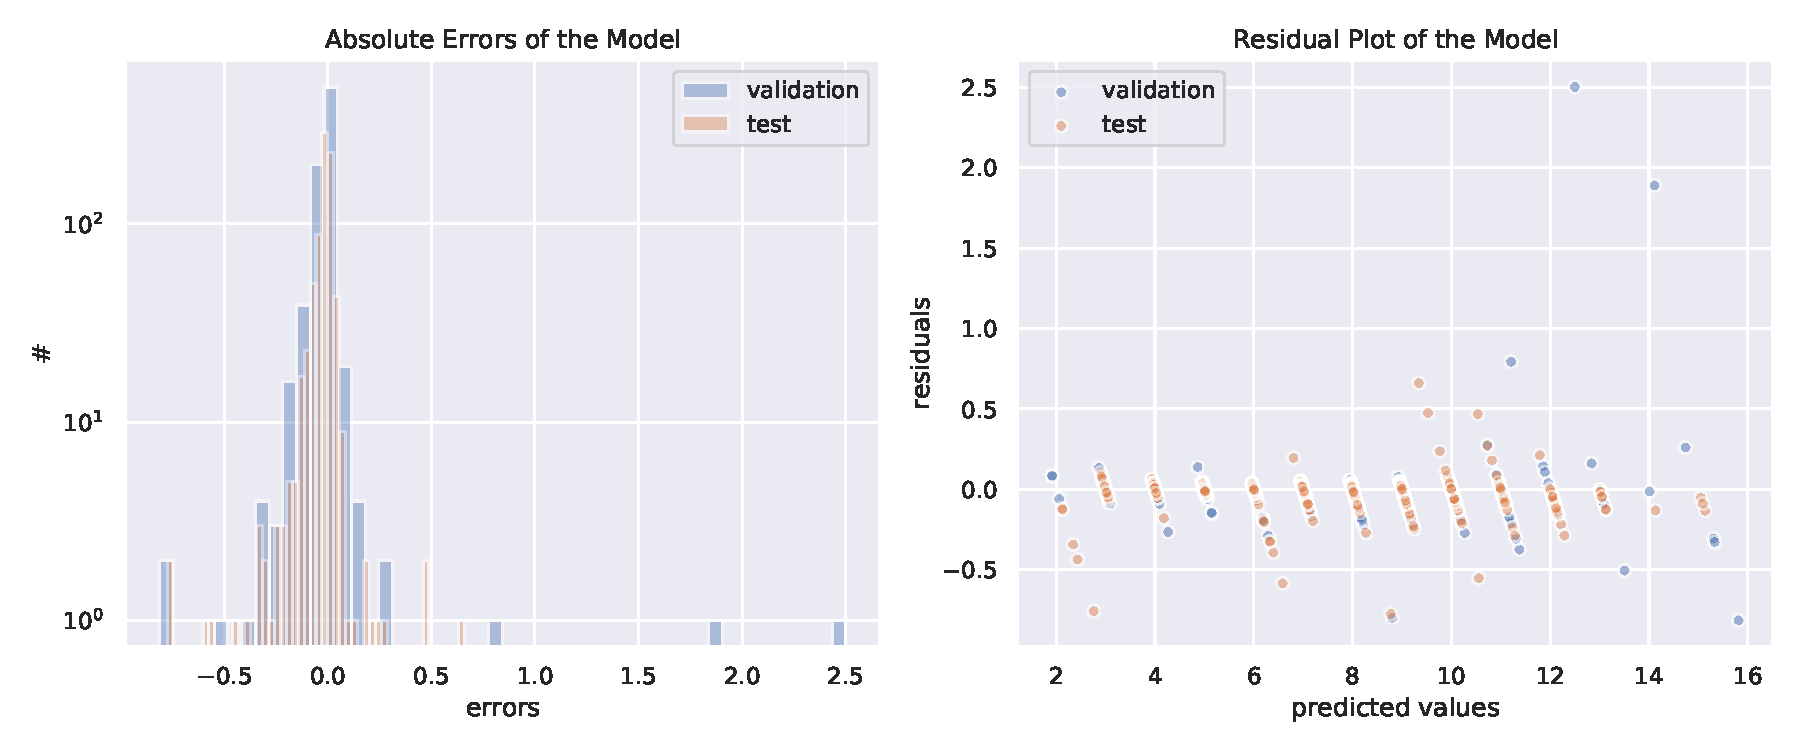
\includegraphics[width=0.8\linewidth]{img/errors_icnn_h11_orig}
    \caption{Residuals of \hodge{1}{1}.}
  \end{subfigure}
  \hfill
  \begin{subfigure}[c]{\linewidth}
    \centering
    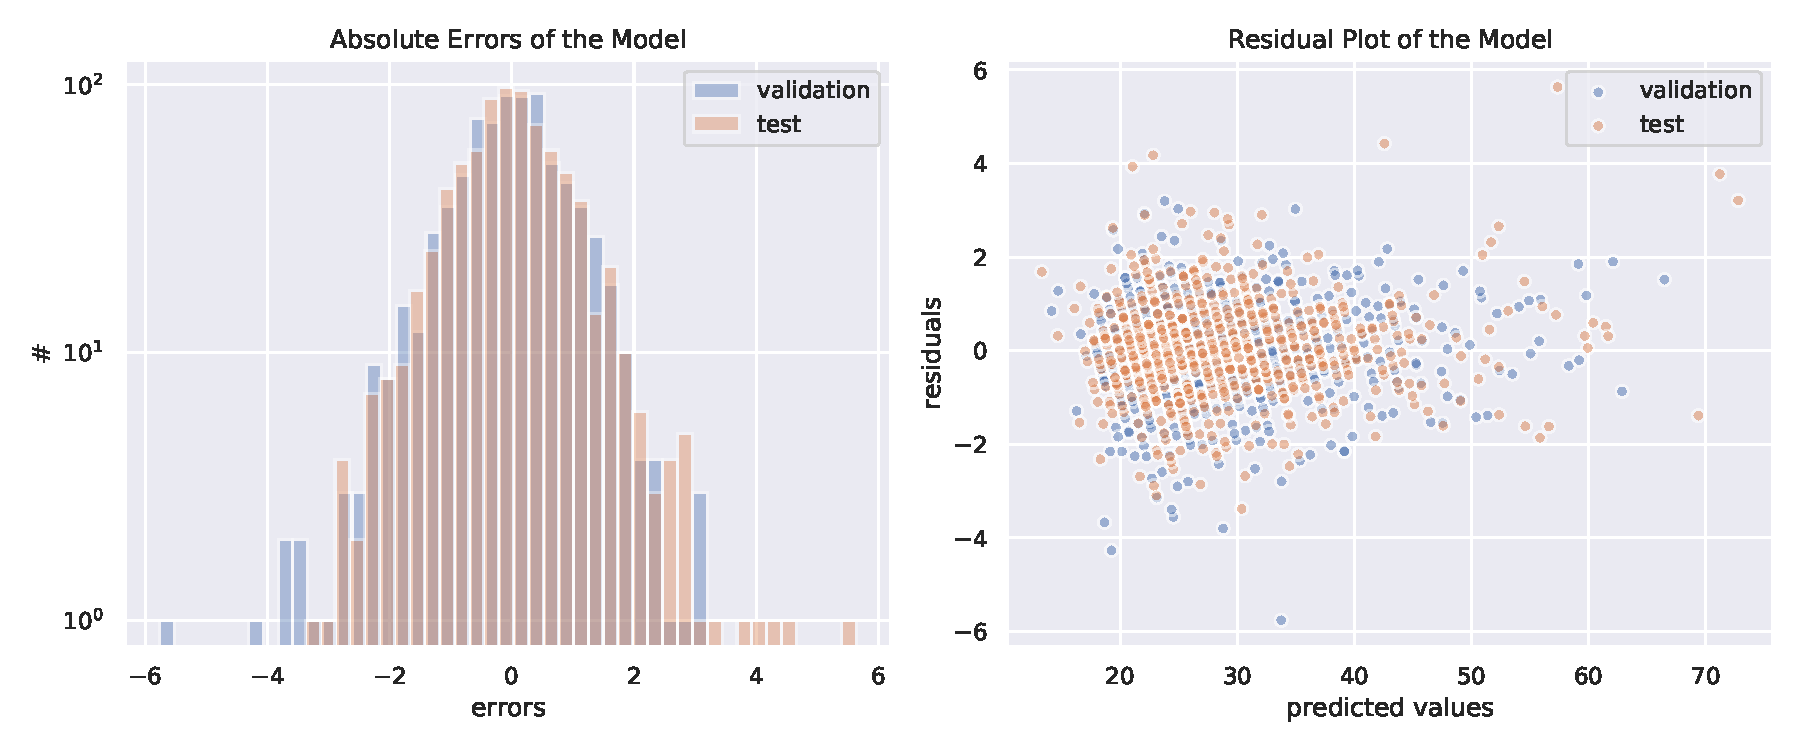
\includegraphics[width=0.8\linewidth]{img/errors_icnn_h21_orig}
    \caption{Residuals of \hodge{2}{1}.}
  \end{subfigure}
  \caption{%
    Histograms of the residual errors and residual plots of the Inception network.
  }
  \label{fig:nn:inception_errors}
\end{figure}

\begin{figure}[tbp]
  \centering
  \begin{subfigure}[c]{0.45\linewidth}
    \centering
    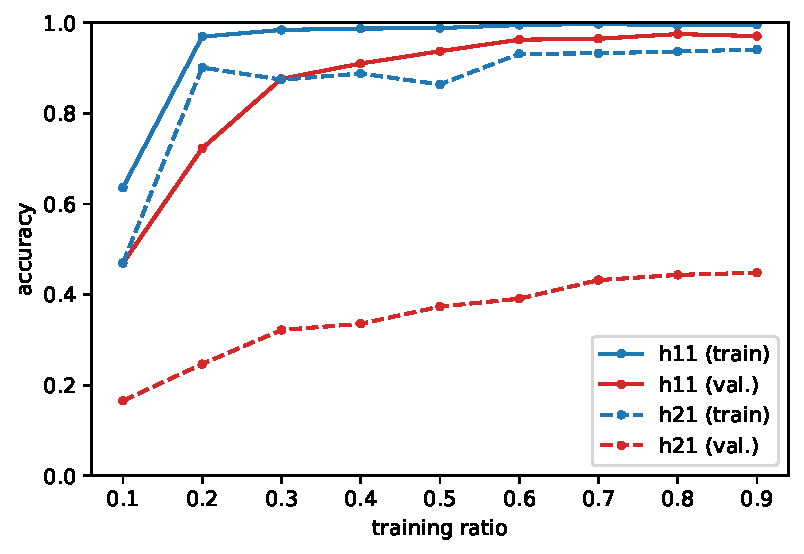
\includegraphics[width=\linewidth]{img/inc_nn_learning_curve}
    \caption{predicting both \hodge{1}{1} and \hodge{2}{1}}
  \end{subfigure}
  \hfill
  \begin{subfigure}[c]{0.45\linewidth}
    \centering
    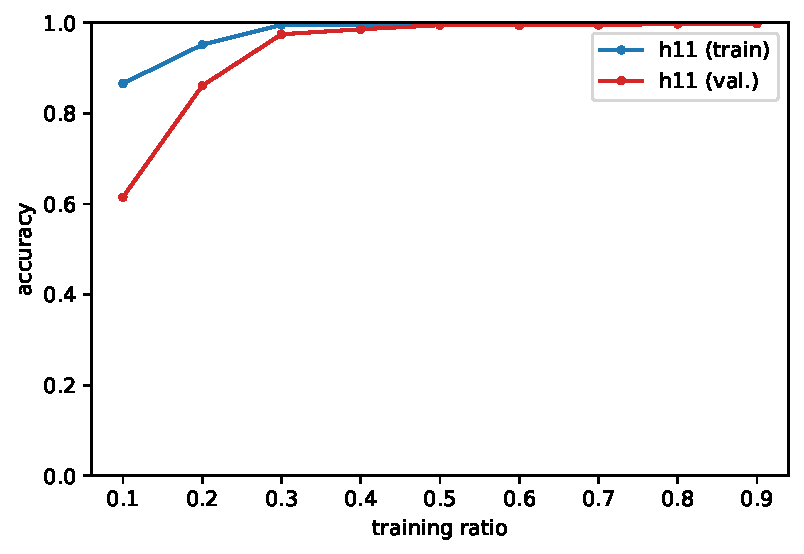
\includegraphics[width=\linewidth]{img/inc_nn_learning_curve_h11}
    \caption{predicting \hodge{1}{1} only}
  \end{subfigure}
  \caption{Learning curves for the Inception neural network (original dataset).}
  \label{fig:lc:inception}
\end{figure}

\begin{table}[htb]
  \centering
  \begin{tabular}{@{}ccccccc@{}}
    \toprule
    & \multicolumn{2}{c}{\textbf{DenseNet}}
    & \multicolumn{2}{c}{\textbf{classic ConvNet}}
    & \multicolumn{2}{c}{\textbf{inception ConvNet}}
    \\
    & \emph{old} & \emph{fav.}
    & \emph{old} & \emph{fav.}
    & \emph{old} & \emph{fav.}
    \\
    \midrule
    \hodge{1}{1}
    & \SI{77}{\percent}  & \SI{97}{\percent}
    & \SI{94}{\percent}  & \SI{99}{\percent}
    & \SI{99}{\percent}  & \SI{99}{\percent}
    \\
    \hodge{2}{1}
    & -     & -
    & \SI{36}{\percent}  & \SI{31}{\percent}
    & \SI{50}{\percent}  & \SI{48}{\percent}
    \\
    \bottomrule
  \end{tabular}
  \caption{%
    Accuracy using \emph{rint} rounding on the predictions of the ANNs on \hodge{1}{1} and \hodge{2}{1} on the test set.
  }
  \label{tab:res:ann}
\end{table}


\subsubsection{Boosting the Inception-like Model}

To improve further the accuracy of \hodge{2}{1} we modify the network by adding engineered features as auxiliary inputs.
This can be done by adding inputs to the inception neural network and merging the different branches at different stages.
There are two possibilities to train such a network: train the whole network directly or train the inception network alone, then freeze its weights and connect it to the additional inputs, training only the new layer.
We found that the architectures we tried did not improve the accuracy, but we briefly describe our attempts for completeness.
We focused in particular on the number of projective spaces, the vector of dimensions of the projective spaces and the vector of dimensions of the principal cohomology group) and predicting \hodge{1}{1} and \hodge{2}{1} at the same time.
The core of the neural network is the Inception network described earlier in~\Cref{sec:ml:nn:inception}.
The engineered features are processed using fully connected layers and merged to the predictions from the Inception branch using a concatenation layer.
Obviously output layers for \hodge{1}{1} and \hodge{2}{1} can be located on different branches which allow for different processing of the features.

As mentioned earlier, a possible approach is to first train the Inception branch alone, before freezing its weights and connecting it to the rest of the network.
This can prevent spoiling the already good predictions and speed up the new learning process.
This is a common technique called \emph{transfer learning}: we can use a model previously trained on a slightly different task and use its weights as part of the new architecture.
Our trials involved shallow fully connected layers ($1$ to $3$ layers with $10$ to $150$ units) between the engineered features and after the concatenation layer.
Since the \eda analysis in~\Cref{sec:data:eda} shows a correlation between both Hodge numbers, we tried architectures where the result for \hodge{1}{1} is used to predict \hodge{2}{1}.
For the training phase we also tried an alternative to the canonical choice of optimising the sum of the losses.
We first train the network and stop the process when the validation loss for \hodge{1}{1} does not longer improve, load back the best weights and save the results, keep training and stop when the loss for \hodge{2}{1} reaches a plateau.

With this setup we were able to slightly improve the predictions of \hodge{1}{1} in the original dataset, reaching almost \SI{100}{\percent} of accuracy in the predictions, while the favourable dataset stayed at around \SI{99}{\percent} of accuracy.
The only few missed predictions (\num{4} manifolds out of \num{786} in the test set) are in very peculiar regions of the distribution of the Hodge number.
For \hodge{2}{1} no improvement has been noticed.


\subsection{Ensemble Learning: Stacking}

We conclude the \ml analysis by describing a method very popular in \ml competitions: ensembling.
This consists in taking several \ml algorithms and combining together the predictions of each individual model to obtain a more precise predictions.
Using this technique it is possible to decrease the variance and improve generalization by compensating weaknesses of algorithms with strengths of others.
Indeed the idea is to put together algorithms which perform best in different zones of the label distribution in order to combine them to build an algorithm better than any individual component.
The simplest such algorithm is \emph{stacking} whose principle is summarised in~\Cref{fig:stack:def}.
First the original training set is split in two parts (not necessarily even).
Second a certain number of \emph{first-level learners} is trained over the first split and used to generate predictions over the second split.
Third a ``meta learner'' is trained of the second split to combine the predictions from the first-level learners.
Predictions for the test set are obtained by applying both level of models one after the other.

We have selected the following models for the first level: linear regression, \svm with the Gaussian kernel, the random forest and the ``inception'' neural network.
The meta-learner is a simple linear regression with $\ell_1$ regularisation (Lasso).
The motivations for the first-level algorithms is that stacking works best with a group of algorithms which work in the most diverse way among them.
Also in this case, we use a cross-validation strategy with 5 splits for each level of the training: from \SI{90}{\percent} of total training set, we split into two halves containing each \SI{45}{\percent} of the total samples and then use 5 splits to grade the algorithm, thus using \SI{9}{\percent} of each split for cross correlation at each iteration) and the Bayes optimisation for all algorithms but the \ann (50 iterations for elastic net, \svm and lasso and 25 for the random forests).
The \ann was trained using a holdout validation set containing the same number of samples as each cross-validation fold, namely \SI{9}{\percent} of the total set.
The accuracy is then computed as usual using \texttt{numpy.rint} for \svm, neural networks, the meta learner and \hodge{1}{1} in the original dataset in general, and \texttt{numpy.floor} in the other cases.

In~\Cref{tab:res:stack}, we show the accuracy of the ensemble learning.
We notice that accuracy improves slightly only for \hodge{2}{1} (original dataset) compared to the first-level learners.
However this is much lower than what has been achieved in~\Cref{sec:ml:nn:inception}.
The reason is that the learning suffers from the reduced size of the training set.
Another reason is that the different algorithms may perform similarly well in the same regions.

\begin{figure}[tbp]
  \centering
  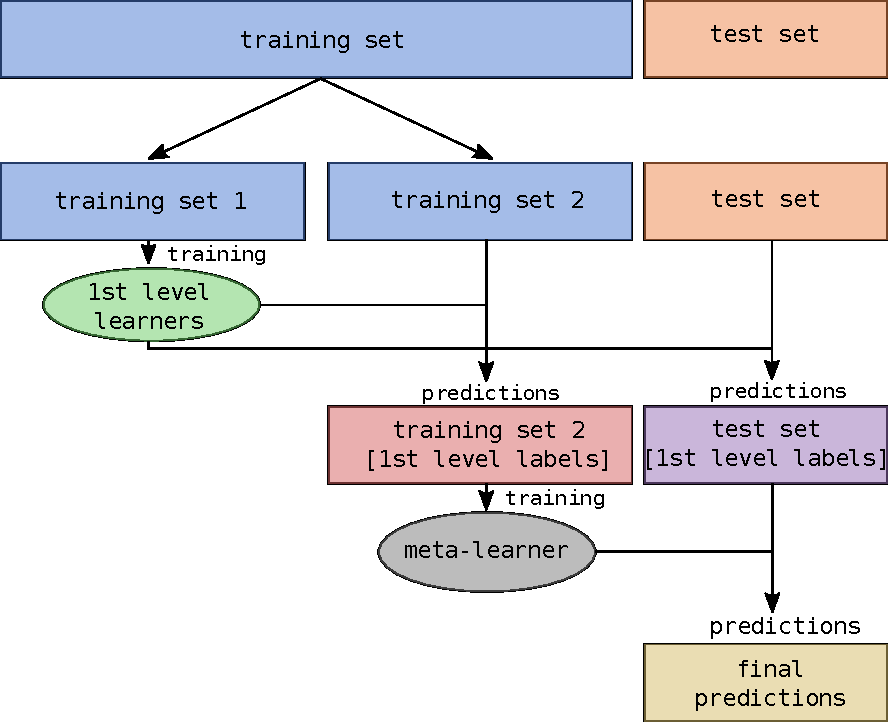
\includegraphics[width=0.65\linewidth]{img/stacking}
  \caption{Stacking ensemble learning with two level learning.}
  \label{fig:stack:def}
\end{figure}

\begin{table}[tbp]
  \centering
  \begin{tabular}{@{}cccccc@{}}
    \toprule
    &
    & \multicolumn{2}{c}{\hodge{1}{1}}
    & \multicolumn{2}{c}{\hodge{2}{1}}
    \\
    &
    & \emph{old}   & \emph{fav.}
    & \emph{old}   & \emph{fav.}
    \\
    \midrule
    \multirow{4}{*}{\emph{1st level}}
    & \textsc{en}
        & \SI{65}{\percent}  & \SI{100}{\percent}
        & \SI{19}{\percent}  & \SI{19}{\percent}
    \\
    & \svm
        & \SI{70}{\percent}  & \SI{100}{\percent}
        & \SI{30}{\percent}  & \SI{34}{\percent}
    \\
    & \textsc{rf}
        & \SI{61}{\percent}  & \SI{98}{\percent}
        & \SI{18}{\percent}  & \SI{24}{\percent}
    \\
    & \ann
        & \SI{98}{\percent}  & \SI{98}{\percent}
        & \SI{33}{\percent}  & \SI{30}{\percent}
    \\
    \midrule
    \multirow{1}{*}{\emph{2nd level}}
    & Lasso
        & \SI{98}{\percent}  & \SI{98}{\percent}
        & \SI{36}{\percent}  & \SI{33}{\percent}
    \\
    \bottomrule
  \end{tabular}
  \caption{%
    Accuracy of the first and second level predictions of the stacking ensemble for elastic net regression (\textsc{en}), support vector with \texttt{rbf} kernel (\svm), random forest (\textsc{rf}) and the artificial neural network (\ann) as first level learners and lasso regression as meta learner.
  }
  \label{tab:res:stack}
\end{table}


% vim: ft=tex
